% Poly "Equations différentielles" -- Mines Paris, UE11
% Compilation : pdflatex poly.tex (x2)   ou   latexmk -pdf poly.tex
% Contenu : traduction directe des sources markdown (chapitres/EDI.tex, chapitres/EDII.tex).
\PassOptionsToPackage{unicode}{hyperref}
\PassOptionsToPackage{hyphens}{url}
\documentclass[french,a4paper,11pt,open=any,headings=small]{scrbook}
\usepackage[a4paper,left=2.5cm,right=2.5cm,top=2.5cm,bottom=3.4cm,footskip=1cm]{geometry}
\usepackage{lmodern}
\usepackage{amssymb,amsmath}
\usepackage[T1]{fontenc}
\usepackage[utf8]{inputenc}
\usepackage{textcomp}
\IfFileExists{upquote.sty}{\usepackage{upquote}}{}
\IfFileExists{microtype.sty}{%
  \usepackage[]{microtype}
  \UseMicrotypeSet[protrusion]{basicmath}
}{}
\usepackage{xcolor}
\IfFileExists{xurl.sty}{\usepackage{xurl}}{}
\usepackage{bookmark}
\hypersetup{
  pdftitle={Equations différentielles},
  pdfauthor={UE11, Mines Paris - PSL},
  pdflang={fr},
  hidelinks}
\urlstyle{tt}
\usepackage{graphicx}
\makeatletter
\def\maxwidth{\ifdim\Gin@nat@width>\linewidth\linewidth\else\Gin@nat@width\fi}
\def\maxheight{\ifdim\Gin@nat@height>\textheight\textheight\else\Gin@nat@height\fi}
\makeatother
\setkeys{Gin}{width=\maxwidth,height=0.36\textheight,keepaspectratio}
\graphicspath{{images/}}
\makeatletter
\def\fps@figure{htbp}
\makeatother
\renewcommand{\topfraction}{0.85}\renewcommand{\bottomfraction}{0.7}\renewcommand{\textfraction}{0.1}\renewcommand{\floatpagefraction}{0.75}
\setlength{\emergencystretch}{3em}
\providecommand{\tightlist}{%
  \setlength{\itemsep}{0pt}\setlength{\parskip}{0pt}}
\setcounter{secnumdepth}{2} % chapitres, sections, sous-sections numérotés
\DeclareOldFontCommand{\rm}{\normalfont\rmfamily}{\mathrm} % les sources utilisent {\rm ...}
\usepackage{fontawesome}
\usepackage{grffile}
\usepackage[shorthands=off,main=french]{babel}
\frenchbsetup{StandardLists=true} % puces standard (et non tirets) pour itemize
\newlength{\cslhangindent}
\setlength{\cslhangindent}{1.5em}
\newenvironment{cslreferences}%
  {\setlength{\parindent}{0pt}%
  \everypar{\setlength{\hangindent}{\cslhangindent}}\ignorespaces}%
  {\par}

% ---- Environnements (définitions, théorèmes, ...) : sobres, sans couleur ----
\usepackage[most]{tcolorbox}
\tcbset{envbase/.style={enhanced,breakable,sharp corners,boxrule=0pt,frame hidden,colback=white,
  left=9pt,right=0pt,top=2pt,bottom=2pt,before skip=1.1\baselineskip,after skip=1.1\baselineskip,
  before upper={\let\footnote\tcbfootnote \setlength{\parindent}{0pt}\setlength{\parskip}{0.5\baselineskip}}}}
% Notes de bas de page dans les environnements : renvoyées en bas de page
% (par défaut tcolorbox les place en fin de boîte, avec des lettres).
\usepackage{etoolbox}
\newcommand{\tcbfnlist}{}
\newcommand{\tcbfootnote}[1]{%
  \stepcounter{footnote}%
  \edef\tcbtmp{\noexpand\footnotetext[\the\value{footnote}]}%
  \expandafter\gappto\expandafter\tcbfnlist\expandafter{\tcbtmp{#1}}%
  \footnotemark[\value{footnote}]}
\newcommand{\tcbflushfn}{\tcbfnlist\gdef\tcbfnlist{}}

\newtcolorbox{definition}[1][]{envbase,borderline west={1.2pt}{0pt}{black},
  before upper={\let\footnote\tcbfootnote \textbf{Définition\IfValueT{#1}{\ -- #1}.}\par\setlength{\parindent}{0pt}\setlength{\parskip}{0.5\baselineskip}}}
\newtcolorbox{theoreme}[1][]{envbase,borderline west={1.2pt}{0pt}{black},
  before upper={\let\footnote\tcbfootnote \textbf{Théorème\IfValueT{#1}{\ -- #1}.}\par\setlength{\parindent}{0pt}\setlength{\parskip}{0.5\baselineskip}\itshape}}
\newtcolorbox{remarque}[1][]{envbase,
  before upper={\let\footnote\tcbfootnote \textbf{Remarque\IfValueT{#1}{\ -- #1}.}\par\setlength{\parindent}{0pt}\setlength{\parskip}{0.5\baselineskip}}}
\newtcolorbox{exemple}[1][]{envbase,
  before upper={\let\footnote\tcbfootnote \textbf{Exemple\IfValueT{#1}{\ -- #1}.}\par\setlength{\parindent}{0pt}\setlength{\parskip}{0.5\baselineskip}}}
\newtcolorbox{preuve}{envbase,left=0pt,
  before upper={\let\footnote\tcbfootnote \setlength{\parindent}{0pt}\setlength{\parskip}{0.5\baselineskip}\textit{Démonstration.}\ }}

\AfterEndEnvironment{definition}{\tcbflushfn}\AfterEndEnvironment{theoreme}{\tcbflushfn}\AfterEndEnvironment{remarque}{\tcbflushfn}\AfterEndEnvironment{exemple}{\tcbflushfn}\AfterEndEnvironment{preuve}{\tcbflushfn}

% Pas de saut de page avant les chapitres
\makeatletter
\patchcmd{\scr@startchapter}{\if@openright\cleardoublepage\else\clearpage\fi}{\par\addpenalty{-300}}{}{\PackageWarning{poly}{patch chapitre echoue}}
\makeatother
\renewcommand*{\chapterpagestyle}{headings}
\RedeclareSectionCommand[beforeskip=1.8\baselineskip,afterskip=1\baselineskip]{chapter}
% Titres de niveau subsubsection ("Question n", "Exercice -- ...") en ligne avec le texte qui suit, moins d'espace autour
\RedeclareSectionCommand[runin=true,beforeskip=0.7\baselineskip,afterskip=0.6em]{subsubsection}

% ---- Macros communes aux deux cours ----
\newcommand{\N}{\mathbb{N}}
\newcommand{\Z}{\mathbb{Z}}
\newcommand{\Q}{\mathbb{Q}}
\newcommand{\R}{\mathbb{R}}
\newcommand{\C}{\mathbb{C}}
\newcommand{\Rgeq}{\R_{\geq 0}}
\newcommand{\Rg}{\R_{> 0}}
% ---- Macros de Equations Différentielles I ----
\newcommand{\cS}{\mathcal{S}}
\newcommand{\cC}{\mathcal{C}}
\newcommand{\inter}{\mathop{\rm int}\nolimits}
\newcommand{\tmin}{t_m^-}
\newcommand{\tmax}{t_m^+}
% ---- Macros de Equations Différentielles II ----
\newcommand{\dt}{{\Delta t}}

% ---- Corrections des exercices : \correctionstrue pour les inclure, \correctionsfalse pour un poly sans corrigés ----
\newif\ifcorrections
% Par défaut avec corrections. Sans les recompiler à la main, une version sans corrections s'obtient par :
%   latexmk -pdf -jobname=poly_sans_corrections -usepretex="\def\sanscorrections{1}" poly.tex
\ifdefined\sanscorrections \correctionsfalse \else \correctionstrue \fi
% Renvoi vers la solution d'un exercice, affiché seulement si les corrections sont incluses
\newcommand{\solref}[1]{\ifcorrections\ (\protect\hyperlink{#1}{Solution p. \pageref*{#1}}.)\fi}

\title{Equations différentielles}
\author{UE11, Maths 2 \\
	Mines Paris - PSL\\~\\
	Pauline Bernard\footnote{Ce document est un des produits
  du projet \href{https://github.com/}{\(\mbox{\faGithub}\)
  \texttt{paulinebernard/CDIS}} issu de la collaboration de
  \href{mailto:pauline.bernard@minesparis.psl.eu}{Pauline Bernard}
  (CAS), \href{mailto:thomas.romary@minesparis.psl.eu}{Thomas
  Romary} et \href{mailto:mike.perreira@minesparis.psl.eu}{Mike Perreira} (GEOSCIENCES). 
%Il dérive du projet
%  \href{https://github.com/}{\(\mbox{\faGithub}\)
%  \texttt{boisgera/CDIS}}, initié par la collaboration de
%  \href{mailto:sebastien.boisgerault@mines-paristech.fr}{(S)ébastien
%  Boisgérault} (CAOR),
%  \href{mailto:thomas.romary@mines-paristech.fr}{(T)homas Romary} et
%  \href{mailto:emilie.chautru@mines-paristech.fr}{(E)milie Chautru}
%  (GEOSCIENCES),
%  \href{mailto:pauline.bernard@mines-paristech.fr}{(P)auline Bernard}
%  (CAS), avec la contribution de
%  \href{mailto:gabriel-stolz@mines-paristech.fr}{Gabriel Stoltz} (Ecole
%  des Ponts ParisTech, CERMICS). 
  Il est mis à disposition selon les
  termes de \href{http://creativecommons.org/licenses/by-nc-sa/}{la
  licence Creative Commons ``attribution -- pas d'utilisation
  commerciale -- partage dans les mêmes conditions'' 4.0
  internationale}.}}
\date{\today}

\counterwithin*{chapter}{part} % la numérotation des chapitres repart à 1 dans chaque partie
\renewcommand{\theHchapter}{\thepart.\arabic{chapter}}

\begin{document}
\maketitle

\setcounter{tocdepth}{2}
\tableofcontents

\part{Etude théorique des solutions}
\hypertarget{un-peu-dhistoire}{%
\chapter{Un peu d'histoire}\label{un-peu-dhistoire}}

L'étude des équations différentielles remonte au XVII\(^e\) siècle lors
de la découverte du calcul infinitésimal et de la modélisation du
mouvement par Kepler et Newton. Avec Leibniz, leur premier réflexe est
alors de chercher à résoudre ces équations de manière exacte, par
exemple par des primitives de fonctions connues ou bien sous forme de
série, mais ces méthodes atteignent vite leurs limites, sauf dans des
cas très particuliers.

Alors que l'idée d'approximer les solutions apparaît au milieu du
XVIII\(^e\) siècle avec Euler, on cherche ensuite plutôt à caractériser
leurs propriétés sans les connaître explicitement. Cauchy, et
parallèlement Lipschitz, démontrent les premiers, au milieu du XIX\(^e\)
siècle, l'existence et l'unicité des solutions sous des hypothèses de
régularités de l'équation différentielle. Laplace, qui s'intéresse alors
à la mécanique céleste, s'émerveille devant la capacité de l'Homme à
prédire l'évolution du monde physique. C'est l'avènement du
\emph{déterminisme} c'est-à-dire la certitude que l'état du monde futur
(ou passé) peut être prédit de manière unique par la connaissance de
l'état initial.

Cependant, à la fin du XIX\(^e\) siècle, les travaux de Poincaré et de
ses contemporains mettent en évidence les limites de ce déterminisme. Le
constat que le modèle physique n'est jamais exactement connu, ni sa
condition initiale, amène les scientifiques à étudier la sensibilité des
solutions à ces erreurs. Une sensibilité extrême chez certains systèmes
rend leur simulation impossible sur des temps longs et mène à la théorie
du \emph{chaos} qui occupera les scientifiques durant une grande partie
du XX\(^e\) siècle.

En parallèle, l'étude de la stabilité et du comportement asymptotique
des solutions intéresse dès le XIX\(^e\) siècle, d'abord dans le cas des
systèmes linéaires avec des mathématiciens comme Routh, Hurwitz, etc.
Mais c'est finalement la thèse de Lyapunov à la fin du XIX\(^e\) siècle
qui lance la théorie générale de la stabilité des systèmes non linéaires
qui sera ensuite étayée tout au long des XX\(^e\) et XXI\(^e\) siècles.

\hypertarget{objectifs-du-cours}{%
\chapter{Objectifs du cours}\label{objectifs-du-cours}}

Ce cours est une introduction à l'étude non linéaire des équations
différentielles. Pour une étude plus complète voir par exemple (Hale
\protect\hyperlink{ref-Hale}{2009}). En première lecture, les objectifs
``opérationnels'' sont les suivants~:

\begin{itemize}
\item
  savoir réduire une équation différentielle à l'ordre 1.
\item
  savoir justifier l'existence de solutions par le théorème de Peano
  lorsque ``\(f\) est continue''.
\item
  comprendre la notion de solution maximale et savoir qu'elles sont
  définies tant qu'elles ``n'explosent'' pas et tant qu'elles
  n'atteignent pas la frontière du domaine où l'équation différentielle
  est définie. Savoir justifier qu'une solution est définie sur tout
  l'intervalle de temps \(\mathbb{R}\) si ces éventualités ne peuvent se
  réaliser en temps fini et/ou en faisant appel au critère
  ``linéairement borné''.
\item
  savoir justifier l'unicité des solutions maximales par le théorème de
  Cauchy-Lipschitz lorsque ``\(f\) est continûment différentiable par
  rapport à \(x\)''.
\item
  comprendre (qualitativement) dans quelle mesure une erreur sur la
  condition initiale se répercute sur les solutions en temps fini.
\item
  savoir trouver les points d'équilibre.
\item
  savoir déterminer si un système linéaire est globalement
  asymptotiquement stable en regardant le signe de la partie réelle de
  ses valeurs propres.
\item
  savoir déterminer si un point d'équilibre est localement
  asymptotiquement stable/instable par les valeurs propres de la matrice
  Jacobienne associée.
\item
  savoir montrer la stabilité d'un point d'équilibre par la décroissance
  d'une fonction définie positive.
\item
  savoir montrer la bornitude des solutions en temps positif lorsque
  cette fonction décroissante est propre.
\item
  savoir étudier la convergence des solutions vers un point d'équilibre
  par l'application répétée du lemme de Barbalat.
\end{itemize}

En deuxième lecture~:

\begin{itemize}
\item
  comprendre la preuve du théorème de Cauchy-Lipschitz en voyant la
  solution comme un point fixe de la représentation intégrale des
  solutions.
\item
  savoir que l'on peut relâcher l'hypothèse du théorème de
  Cauchy-Lipschitz à ``\(f\) lipschitzienne par rapport à \(x\)''.
\item
  comprendre ce qu'est un système chaotique et ce que représente son
  exposant de Lyapunov.
\item
  comprendre ce que la notion de stabilité apporte en plus de
  l'attractivité dans la notion de stabilité asymptotique.
\item
  connaître, comprendre et savoir appliquer les critères de stabilité de
  Lyapunov.
\end{itemize}

\textbf{Notations}

\begin{itemize}
\item
  \(B(x,r)\)~: boule ouverte centrée en \(x\) et de rayon \(r\).
\item
  \(B_f(x,r)\)~: boule fermée centrée en \(x\) et de rayon \(r\).
\item
  Pour \(x:I\subset\mathbb{R}\to \mathbb{R}^n\),
  \(\dot{x}(t)=\frac{dx}{dt}(t)\) et
  \(\ddot{x}(t)=\frac{d^2x}{dt^2}(t)\).
\end{itemize}

\hypertarget{cadre-de-luxe9tude}{%
\chapter{Cadre de l'étude}\label{cadre-de-luxe9tude}}

Les équations différentielles apparaissent couramment en physique pour
décrire l'évolution des grandeurs décrivant le système. Quelques exemples:
\begin{itemize}
\tightlist
\item
  La tension \(u_c\) aux bornes d'un condensateur dans un circuit RLC en
  série évolue selon \[
  \ddot{u}_c = -\frac{R}{L} \dot{u}_c - \frac{1}{LC} u_c + u(t)
  \] où \(R\), \(L\), \(C\) notent la résistance, inductance et capacité
  respectivement, et \(u\) la tension appliquée par le générateur. Cette
  équation différentielle implique les dérivées de \(u_c\) jusqu'à
  l'ordre 2, donc on parle d'équation différentielle d'ordre 2.
\item
  En cinétique chimique, les concentrations des espèces chimiques
  intervenant dans une réaction \[
  A+ B \overset{k}{\underset{k'}{\leftrightarrows}}  C 
  \] sont régies par une équation différentielle d'ordre 1 donnée par
  \begin{align*}
  \dot{c}_A &= -k \, c_Ac_B + k'c_C \\
  \dot{c}_B &= -k \, c_Ac_B + k'c_C\\
  \dot{c}_C &= k \, c_Ac_B - k'c_C
  \end{align*} avec \(k,k'\) les constantes de réaction. Cette équation
  différentielle n'a pas de terme extérieur variant avec le temps. On
  dit qu'elle est \emph{autonome}.
\item
  La mécanique Newtonienne ou Lagrangienne amène typiquement à des
  équations du type \[
  M \ddot{q} = \sum_k F_k(t,q,\dot{q})
  \] où \(q\in \mathbb{R}^n\) modélise la position du système (spatiale,
  angulaire, etc), \(\dot{q}\) sa vitesse et \(\ddot{q}\) son
  accélération, avec \(M\) la matrice d'inertie, et \(F_k\) les
  forces/couples agissant sur le système. Ici il s'agit d'une équation
  différentielle d'ordre 2.
\end{itemize}

Dans tous ces cas, on s'intéresse aux signaux du temps \(t\mapsto y(t)\)
de classe \(C^p\) qui vérifient une équation du type \[
y^{(p)}(t) = \psi\left(t,y(t),\dot{y}(t),\ldots, y^{(p-1)}(t)\right)
\] sur son ensemble de définition, où \(p\in \mathbb{N}^*\) désigne
l'ordre de l'équation différentielle. En fait, on se rend compte que
\(y\) de classe \(C^p\) vérifie l'équation différentielle ci-dessus si
et seulement si \(x=(y,\dot{y},\ldots,y^{(p-1)})\) de classe \(C^1\)
vérifie \[
\dot{x} = f(t,x) \ , 
\] où \(f\) est définie par \[
f(t,y_0,y_1,\ldots,y_{p-1}) = (y_1,y_2,\ldots,y_{p-1},\psi(t,y_0,\ldots,y_{p-1})) \ .
\]

Nous déduisons que résoudre une équation différentielle d'ordre \(p\)
est en fait équivalent à résoudre une équation différentielle d'ordre 1,
quitte à considérer comme inconnue la suite des dérivées
\(x=(y,\dot{y},\ldots,y^{(p-1)})\) de classe \(C^1\), au lieu de \(y\)
de classe \(C^p\). \(x\) est appelé l'\emph{état} du système.

\hypertarget{ex_reducOrdre1}{}
\addcontentsline{toc}{subsubsection}{Réduction à l'ordre 1}
\begin{exemple}[Réduction à l'ordre 1]\label{ex_reducOrdre1}
Reprenons les exemples plus haut~:

\begin{itemize}
\tightlist
\item
  pour un circuit RLC, on prend \(x=(u_c,\dot{u}_c)\in \mathbb{R}^2\),
  et \[
  f(t,x_1,x_2) = 
  \left[
    \begin{matrix}
        x_2\\
        -\frac{R}{L} x_2 - \frac{1}{LC} x_1 + u(t)
    \end{matrix}
  \right] \ .
  \]
\item
  en cinétique chimique, \(x=(c_A,c_B,c_C)\in \mathbb{R}^3\) et \[
  f(t,x_1,x_2,x_3) = \left[
    \begin{matrix}
         -k \, x_1x_2 + k'x_3 \\
         -k \, x_1x_2 + k'x_3\\
         k \, x_1x_2 - k'x_3
    \end{matrix}
  \right]
  \]
\item
  en mécanique, \(x=(q,\dot{q})\) et \[
  f(t,x_1,x_2) = 
  \left[
    \begin{matrix}
        x_2\\
        M^{-1} \sum_k F_k(t,x_1,x_2)
    \end{matrix}
  \right] \ .
  \]
\end{itemize}

Ainsi, même si la physique nous donne initialement une équation
différentielle d'ordre supérieur, on pourra toujours se ramener à
l'ordre 1. Cette réduction est cruciale pour l'étudier mathématiquement
ainsi que numériquement, et devra donc être systématique.
\end{exemple}

Commençons par définir le cadre de cette étude.

\hypertarget{solution-dune-uxe9quation-diffuxe9rentielle}{}
\addcontentsline{toc}{subsection}{Solution d'une équation différentielle}
\begin{definition}[Solution d'une équation différentielle]\label{solution-dune-uxe9quation-diffuxe9rentielle}
Soient \(n\in \mathbb{N}^*\), \(J\) ouvert de \(\mathbb{R}\), \(X\)
ouvert de \(\mathbb{R}^{n}\) et \(f:J\times X \to \mathbb{R}^n\) une
application continue. Une fonction \(x:I\to \mathbb{R}^n\) définie sur
un intervalle de temps \(I\subset J\) non réduit\footnote{Certaines
  références autorisent les solutions définies sur un intervalle
  d'intérieur vide, c'est-à-dire réduit à un point, qui sont dites
  ``triviales''. Mais cela n'a pas grand intérêt ici et nous supposons
  donc que les solutions sont définies au moins ``pendant un certain
  temps''.} à un point, est dite solution\footnote{On omet de préciser
  l'intervalle \(I\) sur lequel \(x\) est solution lorsque \(I\) est
  l'ensemble de définition naturel (ou clairement défini) de \(x\).
  Lorsque celui-ci est ambigu ou bien lorsque l'on veut insister sur
  l'intervalle de définition, on dira \emph{solution sur \(I\)}.} de
l'équation différentielle \[
\dot{x} = f(t,x)
\] si \(x\) est continue sur \(I\) avec \(x(t)\in X\) pour tout
\(t\in I\), et de classe \(C^1\) sur \(\mathring{I}\) avec
\(\dot{x}(t) = f(t,x(t))\) pour tout \(t\in \mathring{I}\).

L'équation différentielle est dite \emph{autonome} si l'application
\(f\) ne dépend pas de \(t\). Dans ce cas, on peut aussi définir
directement \(f: X \to \mathbb{R}^n\).

Lorsque l'intervalle de temps \(I\) de définition de la solution est
\(J\) entier, on dira que la solution est \emph{globale}. Mais on verra
qu'il peut parfois arriver qu'une solution ne puisse être définie sur
\(J\) entier, par exemple si elle explose avant, ou si elle s'apprête à
quitter \(X\).
\end{definition}

Notons que \(f\) sera souvent définie sur
\(J\times X=\mathbb{R}\times \mathbb{R}^{n}\). Cependant, il peut
arriver que cela ne soit pas le cas, comme par exemple pour deux corps
de position \(y_a,y_b\) dont la force d'interaction gravitationnelle
\(\frac{Gm_a m_b}{\|y_a-y_b\|^2}\) n'est définie que pour
\(y_a\neq y_b\), où lorsque l'on veut restreindre l'étude des solutions
à un domaine particulier.

La physique s'intéresse souvent aux solutions partant d'une
\emph{condition initiale} donnée. La recherche et l'étude de ces
solutions particulières est due à Cauchy et porte le nom de
\emph{Problème de Cauchy}~:

\begin{quote}
Dans mes leçons données à l'École Polytechnique, comme dans la plupart
des ouvrages ou mémoires que j'ai publiés sur le calcul intégral, j'ai
cru devoir placer en premier lieu la recherche, non pas des intégrales
générales, mais des particulières\,; en sorte que la détermination des
constantes ou des fonctions arbitraires ne fût plus séparée de la
recherche des intégrales.
\end{quote}


\hypertarget{def_cauchy}{}
\addcontentsline{toc}{subsection}{Problème de Cauchy (\emph{Initial Value Problem})}
\begin{definition}[Problème de Cauchy (\emph{Initial Value Problem})]\label{def_cauchy}
Soient \(J\) ouvert de \(\mathbb{R}\), \(X\) ouvert de
\(\mathbb{R}^{n}\), \((t_0,x_0)\in J\times X\) et
\(f: J\times X \to \mathbb{R}^n\) continue. Le \emph{problème de Cauchy}
associé fait référence au système \[
\dot{x}=f(t,x) \quad , \quad x(t_0)=x_0 \ .
\] On dira donc que \(x:I\to \mathbb{R}^n\) est solution du problème de
Cauchy défini par \(f\) et \((t_0,x_0)\) si

\begin{itemize}
\item
  \(t_0\in I\) et \(x(t_0)=x_0\)
\item
  \(x\) est solution de l'équation différentielle \(\dot{x}=f(t,x)\) sur
  \(I\).
\end{itemize}

On notera alors \(x\in S_f(t_0,x_0)\).
\end{definition}

Avant d'étudier les solutions d'un problème de Cauchy, il est crucial de
remarquer la caractérisation qui suit.

\hypertarget{theo_eq_integrale}{}
\addcontentsline{toc}{subsection}{Représentation intégrale des solutions}
\begin{theoreme}[Représentation intégrale des solutions]\label{theo_eq_integrale}
Soient \(J\) ouvert de \(\mathbb{R}\), \(X\) ouvert de
\(\mathbb{R}^{n}\), \(f: J\times X \to \mathbb{R}^n\) continue,
\(I\subset J\) un intervalle de \(\mathbb{R}\) non réduit à un point,
\(t_0\in I\), \(x_0\in X\), et \(x: I\to \mathbb{R}^n\) continue telle
que \(x(t)\in X\) pour tout \(t\in I\). Alors, \(x\) est solution du
problème de Cauchy défini par \(f\) et \((t_0,x_0)\) si et seulement si
\(x\) est solution de l'équation intégrale \[
x(t) = x_0 + \int_{t_0}^t f(s,x(s))ds \qquad \forall t\in I \ .
\]
\end{theoreme}
Notons que cette caractérisation n'aurait pas été possible si l'on avait
gardé une équation différentielle d'ordre \(p>1\).


\hypertarget{duxe9monstration}{}
\begin{preuve}\label{duxe9monstration}
Supposons \(x\in S_f(t_0,x_0)\). Alors \(x: I\to \mathbb{R}^n\) est de
classe \(C^1\) sur \(\mathring{I}\), et pour tout \(t\in I\), \[
x_0 + \int_{t_0}^t f(s,x(s))ds = x(t_0)  + \int_{t_0}^t \dot{x}(s) ds = x(t) \ .
\] Réciproquement, si \(x\) vérifie l'équation intégrale sur
\(I\subset J\), \(x(t_0)=x_0\), et puisque \(f\) est continue sur
\(I\times X\) et \(x\) continue sur \(I\), \(x\) est de classe \(C^1\)
sur \(I\) et par dérivation, \(\dot{x}(t)=f(t,x(t))\) pour tout
\(t\in I\).\hfill$\blacksquare$
\end{preuve}

\hypertarget{classe-plus-guxe9nuxe9rale-de-solutions}{}
\addcontentsline{toc}{subsection}{Classe plus générale de solutions}
\begin{remarque}[Classe plus générale de solutions]\label{classe-plus-guxe9nuxe9rale-de-solutions}
La définition sous forme intégrale des solutions montre que la recherche
de solutions \(C^1\) et l'hypothèse de continuité de \(f\) pourraient
être relâchées~: il suffirait de chercher \(x\) absolument continue et
pouvoir définir l'objet \(\int_{t_0}^t f(s,x(s))ds\). Mais il est tout
de même souhaitable d'assurer un minimum de propriétés telles que
l'existence de solutions, comme nous allons le voir dans la section
suivante.
\end{remarque}

\hypertarget{portrait-de-phase}{%
\begin{remarque}[Portrait de phase]\label{portrait-de-phase}}

En dimension 2 (ou 3), il est possible de visualiser géométriquement le
comportement des solutions en traçant les courbes paramétriques
\(t\mapsto(x_1(t),x_2(t))\) dans le plan (ou
\(t\mapsto(x_1(t),x_2(t),x_3(t))\) dans l'espace) pour différentes
conditions initiales. C'est ce que l'on appelle un \emph{portrait de
phase}. Voir \protect\hyperlink{fig_pendule}{Figure~\ref*{fig_pendule} (p.
\pageref*{fig_pendule})} dans le cas d'un pendule.
\end{remarque}

\begin{figure}
\hypertarget{fig_pendule}{%
\centering
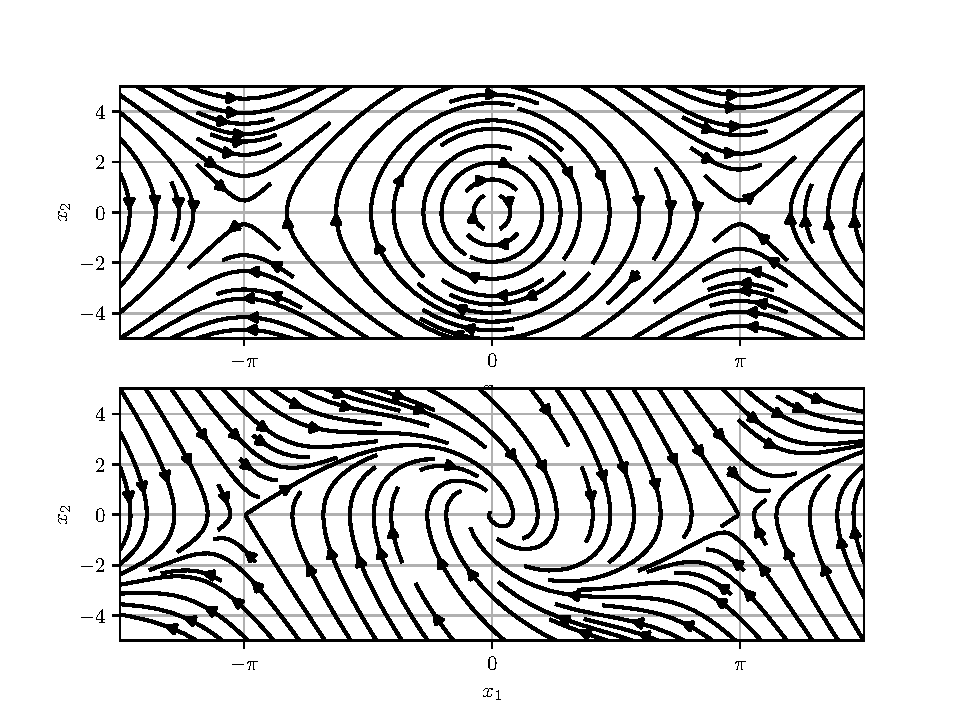
\includegraphics{images/pendule.py.pdf}
\caption{Portraits de phase d'un pendule non amorti en haut et amorti en
bas. \(x_1\) représente l'angle du pendule en abscisse et \(x_2\) sa
vitesse de rotation en ordonnée. Le pendule sera décrit et étudié plus
en détail dans la suite du cours.}\label{fig_pendule}
}
\end{figure}

\hypertarget{etude-du-probluxe8me-de-cauchy}{%
\chapter{Etude du problème de
Cauchy}\label{etude-du-probluxe8me-de-cauchy}}

\hypertarget{existence-de-solutions-locales}{%
\section{Existence de solutions
locales}\label{existence-de-solutions-locales}}

Notre point de départ est le théorème suivant établi à la fin du
XIX\(^e\) siècle, qui assure l'existence locale de solutions au
\protect\hyperlink{def_cauchy}{problème de Cauchy (p.
\pageref*{def_cauchy})} sous une simple hypothèse de continuité de
\(f\). En d'autres termes, dans le cadre de ce cours où \(f\) est
supposée continue, il existe toujours des solutions pour toute condition
initiale, définies au moins pour un certain temps.

\hypertarget{theo_peano}{}
\addcontentsline{toc}{subsection}{Théorème de Peano-Arzelà}
\begin{theoreme}[Théorème de Peano-Arzelà]\label{theo_peano}
Soient \(J\) ouvert de \(\mathbb{R}\), \(X\) ouvert de
\(\mathbb{R}^{n}\), \(f: J\times X \to \mathbb{R}^n\) continue. Pour
tout \((t_0,x_0)\in J\times X\), il existe \(\tau_m >0\) et
\(x :[t_0-\tau_m,t_0+\tau_m]\to\mathbb{R}^n\) tels que \(x\) est
solution du problème de Cauchy défini par \(f\) et \((t_0,x_0)\).
\end{theoreme}

\hypertarget{duxe9monstration-1}{}
\begin{preuve}\label{duxe9monstration-1}
La démonstration de ce résultat est hors-programme et fait appel au
théorème d'Ascoli(-Arzelà). Seule la connaissance et la compréhension du
résultat est exigible. Pour les curieux, la preuve est donnée en
\protect\hyperlink{app_peano}{annexe (p.
\pageref*{app_peano})}.\hfill$\blacksquare$
\end{preuve}

\hypertarget{classe-plus-guxe9nuxe9rale-de-solutions-pour-la-culture}{}
\addcontentsline{toc}{subsection}{Classe plus générale de solutions (pour la culture)}
\begin{remarque}[Classe plus générale de solutions (pour la culture)]\label{classe-plus-guxe9nuxe9rale-de-solutions-pour-la-culture}
L'existence de solutions \(C^1\) est garantie lorsque \(f\) est
continue. Il s'avère que l'existence de solutions \emph{absolument
continues}, est garantie sous les hypothèses plus faibles suivantes dans
un voisinage de \((t_0,x_0)\)~:

\begin{itemize}
\item
  pour tout \(t\), \(x\mapsto f(t,x)\) est continue\,;
\item
  pour tout \(x\), \(t\mapsto f(t,x)\) est mesurable\,;
\item
  il existe une fonction intégrable \(t\mapsto b(t)\) telle que
  \(|f(t,x)|\leq b(t)\) pour tout \((t,x)\).
\end{itemize}

Ce sont les conditions de \emph{Carathéodory}. Voir (Hale
\protect\hyperlink{ref-Hale}{2009}). Un cadre encore plus général
consiste à autoriser des discontinuités de \(f\) par rapport à \(x\)
mais l'étude des solutions passe alors par celle des \emph{inclusions
différentielles} du type \(\dot{x} \in F(t,x)\), ce qui nous amènerait
bien trop loin de ce cours. Voir (Filippov
\protect\hyperlink{ref-Fil}{1988}).
\end{remarque}

\hypertarget{domaine-dexistence-des-solutions}{%
\section{Domaine d'existence des
solutions}\label{domaine-dexistence-des-solutions}}

Nous venons de voir que des solutions locales au problème de Cauchy
existent si \(f\) est continue. Nous savons qu'elles sont définies
\emph{au moins un certain temps}, mais il est intéressant de se demander
quel est l'intervalle de temps \emph{maximal} sur lequel elles peuvent
être définies. En d'autres termes, on s'intéresse aux \emph{solutions
maximales}.

\hypertarget{def_sol_max}{}
\addcontentsline{toc}{subsection}{Solution maximale}
\begin{definition}[Solution maximale]\label{def_sol_max}
Soient \(J\) ouvert de \(\mathbb{R}\), \(X\) ouvert de
\(\mathbb{R}^{n}\), \(f: J\times X \to \mathbb{R}^n\) continue. On dit
que \(x : I \to\mathbb{R}^n\) est une solution \emph{maximale} de
l'équation différentielle \[
\dot{x}=f(t,x)
\] si elle n'est pas \emph{prolongeable} en une solution définie plus
longtemps dans \(J\times X\). En d'autres termes, il n'existe pas de
solution \(x' : I'\to\mathbb{R}^n\) avec \(I\) strictement inclus dans
\(I'\) et telle que \(x=x'\) sur \(I\). On dit alors que \(I\) est
l'\emph{intervalle maximal d'existence} de la solution.
\end{definition}

Il s'avère que l'intervalle maximal de définition \(I\) d'une solution
maximale n'est pas nécessairement \(\mathbb{R}\) entier même si \(f\)
est définie globalement sur \(\mathbb{R}\times \mathbb{R}^n\) et \(f\)
est de classe \(C^\infty\).

\hypertarget{ex_explTempsFini}{}
\addcontentsline{toc}{subsubsection}{Explosion en temps fini}
\begin{exemple}[Explosion en temps fini]\label{ex_explTempsFini}
Considérons le problème de Cauchy \[
\dot{x} = x^2 \quad , \qquad (t_0,x_0)\in \mathbb{R}^2 \ .
\] L'application \(f:(t,x)\mapsto x^2\) est continue sur
\(\mathbb{R}^2\), donc il existe au moins une solution. On peut par
exemple vérifier que, pour \(x_0>0\), \(x:I\to \mathbb{R}\) définie par \[
x(t)=\frac{x_0}{1-x_0(t-t_0)} \quad , \quad I=\left]-\infty,t_0+\frac{1}{x_0}\right[
\] est bien solution. Vu qu'elle diverge au temps \(t_0+\frac{1}{x_0}\),
elle ne peut être prolongée au delà. Elle est donc maximale et on dit
qu'elle \emph{explose en temps fini}. Pour \(x_0<0\), la même formule
définit une solution maximale sur \(I=\left]t_0+\frac{1}{x_0},+\infty\right[\),
qui explose dans le passé, et pour \(x_0=0\) la solution nulle est
définie sur \(\mathbb{R}\) (voir
\protect\hyperlink{fig_explo_temps_fini}{Figure~\ref*{fig_explo_temps_fini}
(p. \pageref*{fig_explo_temps_fini})}).

En fait, le théorème suivant montre que les solutions maximales sont
définies sur un intervalle ouvert, et cet intervalle n'est borné que si
\(t\mapsto x(t)\) diverge en temps fini ou \(t\mapsto(t,x(t))\) tend
vers la frontière de l'ensemble de définition \(J\times X\) de \(f\) en
temps fini.
\end{exemple}

\begin{figure}
\hypertarget{fig_explo_temps_fini}{%
\centering
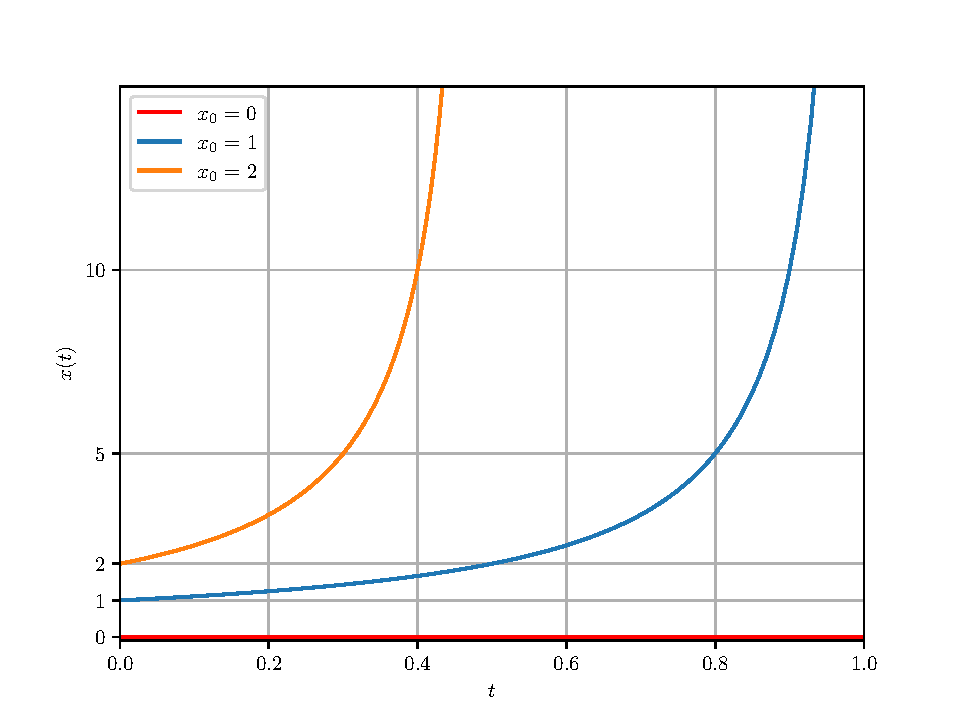
\includegraphics{images/explosion_temps_fini.py.pdf}
\caption{Solutions à \(\dot{x} = x^2\) pour \(t_0=0\) et différentes
valeurs de \(x_0\)}\label{fig_explo_temps_fini}
}
\end{figure}

\hypertarget{theo_bouts}{}
\addcontentsline{toc}{subsection}{Domaine maximal d'existence}
\begin{theoreme}[Domaine maximal d'existence]\label{theo_bouts}
Soient \(J\) ouvert de \(\mathbb{R}\), \(X\) ouvert de
\(\mathbb{R}^{n}\), \(f: J\times X \to \mathbb{R}^n\) continue et
\((t_0,x_0)\in J\times X\). Toute solution du problème de Cauchy défini
par \(f\) et \((t_0,x_0)\) est prolongeable en une solution maximale et
toute solution maximale \(x:I\to \mathbb{R}^n\) est définie sur un
intervalle ouvert \(\left]\tmin,\tmax\right[\) avec
\(\tmin,\tmax\in \mathbb{R}\cup\{+\infty,-\infty\}\). De plus, si
\(\tmax\) (resp. \(\tmin\)) est fini alors \[
\lim_{t\to \tmax} \ \|x(t)\| + \frac{1}{d\Big((t,x(t)),\partial (J\times X) \Big)} = +\infty
\qquad \Big(\text{resp. } \lim_{t\to \tmin}\Big) \ ,
\] avec la convention \(1/d = 0\) si \(\partial (J\times X)=\emptyset\).
Autrement dit, la solution finit par être, à chaque instant, soit très
loin de l'origine, soit très proche de la frontière de \(J\times X\)~:
elle ne peut pas rester dans une région bornée et à distance positive du
bord. En particulier~:

\begin{itemize}
\item
  si \(X=\mathbb{R}^n\) et \(\tmax\) est intérieur à \(J\), seule la
  première possibilité subsiste~: \(\lim_{t\to \tmax}\|x(t)\| = +\infty\),
  la solution \emph{explose en temps fini}~;
\item
  si \(X\) est borné, seule la seconde subsiste~:
  \(\lim_{t\to \tmax} d\big(x(t),\partial X\big) = 0\), la solution
  \emph{atteint le bord en temps fini}.
\end{itemize}
\end{theoreme}

\begin{remarque}[Diverger ou tendre vers le bord\,?]
Attention, la somme tend vers \(+\infty\) sans qu'aucun des deux termes
n'ait forcément de limite~: rien n'empêche en général une solution
d'alterner indéfiniment, en temps fini, entre des passages près de la
frontière et des excursions de plus en plus lointaines. C'est pourquoi on
ne peut pas écrire ``ou bien \(\|x(t)\|\to+\infty\), ou bien \(d\to 0\)''
en dehors des deux cas particuliers ci-dessus.
\end{remarque}

\hypertarget{duxe9monstration-2}{}
\begin{preuve}\label{duxe9monstration-2}
La preuve complète est donnée en
\protect\hyperlink{pr_theo_bouts}{annexe (p. \pageref*{pr_theo_bouts})}.
On commence par observer que si l'intervalle d'existence n'était pas
ouvert, la solution pourrait être prolongée au bord grâce au théorème de
Peano, ce qui contredirait sa maximalité. Ensuite, la preuve consiste à
montrer que si \(\tmax\) (resp. \(\tmin\)) est fini, alors \((t,x(t))\)
finit forcément par sortir définitivement de toute région bornée et à
distance positive du bord de \(J\times X\) (c'est-à-dire de tout
compact de \(J\times X\)) lorsque \(t\) tend vers \(\tmax\) (resp.
\(\tmin\)), ce qui est exactement le contenu de la limite
ci-dessus.\hfill$\blacksquare$

En pratique, pour montrer que les solutions maximales sont définies pour
tout temps, i.e., sur \(\mathbb{R}\), il suffit donc de montrer qu'elles
ne peuvent pas aller arbitrairement loin en temps fini (par exemple si elles sont bornées
sur tout intervalle de temps fini), et qu'elles ne peuvent pas s'approcher arbitrairement proche du bord de \(J\times X\) en temps fini (par exemple si
\(J\times X= \mathbb{R}\times \mathbb{R}^n\)). Un cas particulier où les
solutions maximales sont forcément définies sur \(J\) entier est donné
ci-dessous.
\end{preuve}

\hypertarget{theo_exist_glob}{}
\addcontentsline{toc}{subsection}{Critère d'existence globale}
\begin{theoreme}[Critère d'existence globale]\label{theo_exist_glob}
Soient \(J\) un intervalle ouvert de \(\mathbb{R}\) et
\(f:J\times\mathbb{R}^n\to\mathbb{R}^n\) continue. Si \(f\) a une
\emph{croissance au plus affine}, c'est-à-dire, s'il existe
\(a,b: J\to\mathbb{R}\) continues telles que
\[
\|f(t,x)\|\leq a(t) \|x\| + b(t) \quad \forall (t,x)\in J\times \mathbb{R}^n \ ,
\] alors toute solution maximale est définie sur \(J\) entier.
\end{theoreme}

\hypertarget{duxe9monstration-3}{}
\begin{preuve}\label{duxe9monstration-3}
Prouvé dans l'exercice \protect\hyperlink{exo_gronwall}{\emph{Autour du
Lemme de Grönwall} (p. \pageref*{exo_gronwall})}.\hfill$\blacksquare$
\end{preuve}

\hypertarget{ex_solGlob}{}
\addcontentsline{toc}{subsubsection}{Solutions globales}
\begin{exemple}[Solutions globales]\label{ex_solGlob}
\begin{itemize}
\item
  Considérons une équation différentielle \emph{linéaire}, c'est-à-dire
  pour laquelle il existe \(A:\mathbb{R}\to\mathbb{R}^{n\times n}\) et
  \(b:\mathbb{R}\to\mathbb{R}^n\) continues telles que \[
  f(t,x) = A(t) x + b(t) \ .
  \] D'après le théorème précédent, quelle que soit la condition
  initiale \((t_0,x_0)\in \mathbb{R}\times\mathbb{R}^n\), ses solutions maximales
  sont définies sur \(\mathbb{R}\) entier (on verra dans la suite qu'il en existe
  une unique pour chaque condition initiale). Dans le cas où \(A\) est
  constant, on en a même une formule explicite (obtenue par la méthode
  de \emph{variation de la constante}) \[
  x(t) = e^{A(t-t_0)}x_0 + \int_{t_0}^t e^{A(t-s)} b(s)ds \ ,
  \] où \(e^{A(t-s)}\) est l'exponentielle de matrice définie par \[
  e^{A(t-s)}=\sum^{+\infty}_{p=0} \frac{A^p(t-s)^p}{p!} \ .
  \] Attention, cette formule ne fonctionne que si \(A\) est constant.
  Notons que si \(A\) est diagonalisable, i.e., il existe
  \(P\in \mathbb{R}^{n\times n}\) telle que \(A = P^{-1} D P\) avec
  \(D\in \mathbb{R}^{n\times n}\) une matrice diagonale contenant les
  valeurs propres de \(A\), alors \[
  e^{A(t-s)} = P^{-1} e^{D(t-s)}  P
  \] donc les solutions avec \(b=0\) sont des combinaisons linéaires de
  \(e^{\lambda_i t}\) où \(\lambda_i\) sont les valeurs propres de
  \(A\). Ceci n'est plus vrai lorsque \(A\) n'est pas diagonalisable.
  Voir l'\protect\hyperlink{Hurwitz}{étude de stabilité d'un système
  linéaire (p. \pageref*{Hurwitz})}.
\item
  Un autre cas important d'une croissance au plus affine est lorsque
  \(f\) est globalement bornée en \(x\). Par exemple, \[
  f(t,x)=c(t)\arctan(x) \qquad \text{ ou } \qquad 
  f(t,x)=\frac{c(t)}{1+x^2}
  \] engendrent des problèmes de Cauchy aux solutions globales.
\end{itemize}
\end{exemple}

\hypertarget{glob_sol}{%
\subsubsection*{\texorpdfstring{Exercice -- Solutions globales I
}{Exercice -- Solutions globales I}}\label{glob_sol}}

\addcontentsline{toc}{subsubsection}{Solutions globales I}

Justifier que pour toute condition initiale,
\[
\begin{array}{rcl}
\dot{x}_1 &=& \sin x_1 - \sqrt{|t|} x_2 \\
\dot{x}_2 &=& \sqrt{1+x_1^2}
\end{array}
\] admet des solutions et les solutions maximales sont définies sur
\(\mathbb{R}\).\solref{answer-glob_sol}

\hypertarget{glob_sol2}{%
\subsubsection*{\texorpdfstring{Exercice -- Solutions globales II
(\(\mathord{\bullet}\))}{Exercice -- Solutions globales II (•)}}\label{glob_sol2}}

\addcontentsline{toc}{subsubsection}{Solutions globales II}

Soient \(f:\mathbb{R}\times \mathbb{R}^n \to \mathbb{R}^n\) continue et
\(V:\mathbb{R}^n \to \mathbb{R}\) définie par \(V(x) = x^\top x\) telles
que \[
\langle\nabla V (x), f(t,x)\rangle \leq a(t) V(x) + b(t)  \qquad \forall (t,x)\in \mathbb{R}\times \mathbb{R}^n
\] avec \(a,b:\mathbb{R}\to \mathbb{R}\) continues. Montrer que quelle
que soit la condition initiale
\((t_0,x_0)\in \mathbb{R}\times \mathbb{R}^n\), les solutions maximales
de \(\dot{x} = f(t,x)\) sont définies sur \([t_0,+\infty[\). On pourra
pour cela étudier l'évolution de \(t\mapsto V(x(t))\).\solref{answer-glob_sol2}

\hypertarget{glob_sol3}{%
\subsubsection*{\texorpdfstring{Exercice -- Solutions globales III
(\(\mathord{\bullet}\))}{Exercice -- Solutions globales III (•)}}\label{glob_sol3}}

\addcontentsline{toc}{subsubsection}{Solutions globales III}

Soient \(f:\mathbb{R}\times \mathbb{R}^n \to \mathbb{R}^n\) continue et
\(V:\mathbb{R}^n \to \mathbb{R}\) telle que \[
\lim_{\|x\| \to +\infty} V(x) = +\infty \quad \text{et} \quad \langle\nabla V(x), f(t,x)\rangle \leq 0  \qquad \forall (t,x)\in \mathbb{R}\times \mathbb{R}^n \ .
\] Montrer que quelle que soit la condition initiale
\((t_0,x_0)\in \mathbb{R}\times \mathbb{R}^n\), les solutions maximales
de \(\dot{x} = f(t,x)\) sont définies et bornées sur \([t_0,+\infty[\).
On pourra pour cela étudier l'évolution de \(t\mapsto V(x(t))\).\solref{answer-glob_sol3}

\hypertarget{unicituxe9-des-solutions-maximales}{%
\section{Unicité des solutions
maximales}\label{unicituxe9-des-solutions-maximales}}

Si des solutions maximales existent toujours, elles ne sont pas toujours
uniques.

\hypertarget{ex_nonUnique}{}
\addcontentsline{toc}{subsubsection}{Non-unicité des solutions}
\begin{exemple}[Non-unicité des solutions]\label{ex_nonUnique}
Considérons le problème de Cauchy \[
\dot{x}=-\sqrt{|x|} \qquad , \qquad (t_0,x_0)=(0,0) \ .
\] Ce système permet en particulier de modéliser l'écoulement d'un
fluide dans un réservoir, selon la loi de \emph{Torricelli} (voir
\protect\hyperlink{exo_Torricelli}{exercice (p.
\pageref*{exo_Torricelli})}). La fonction \(f:(t,x)\mapsto -\sqrt{|x|}\)
est continue sur \(\mathbb{R}\times \mathbb{R}\), donc ce problème de
Cauchy admet au moins une solution. Mais on montrera en
\protect\hyperlink{exo_Torricelli}{exercice (p.
\pageref*{exo_Torricelli})} qu'il existe une infinité de solutions
maximales. Plus de détails sont donnés dans le notebook Equations
Différentielles I.ipynb.

Le théorème suivant, dit de \emph{Cauchy-Lipschitz}, montre que
l'unicité des solutions maximales est garantie si \(f\) est de plus
continûment différentiable par rapport à la variable \(x\). On voit que
ce n'est pas le cas de \(x\mapsto -\sqrt{|x|}\) en 0. Le théorème et la
preuve de l'époque sont disponibles en ligne dans des notes de cours
(Moigno \protect\hyperlink{ref-cauchy}{1844}).
\end{exemple}

\hypertarget{theo_lips}{}
\addcontentsline{toc}{subsection}{Théorème de Cauchy-Lipschitz (ou de Picard-Lindelöf)}
\begin{theoreme}[Théorème de Cauchy-Lipschitz (ou de Picard-Lindelöf)]\label{theo_lips}
Soient \(J\) ouvert de \(\mathbb{R}\), \(X\) ouvert de
\(\mathbb{R}^{n}\), \(f: J\times X \to \mathbb{R}^n\) continue et
continûment différentiable par rapport à \(x\),
i.e.~\((t,x)\mapsto \partial_x f(t,x)\) existe et est continue sur
\(J\times X\). Alors pour tout \((t_0,x_0)\in J\times X\), il existe une
unique solution maximale \(x:I\subset J\to\mathbb{R}^n\) au problème de
Cauchy défini par \(f\) et \((t_0,x_0)\).
\end{theoreme}

\hypertarget{duxe9monstration-4}{}
\begin{preuve}\label{duxe9monstration-4}
Nous donnons ici le principe de la preuve qui peut être passée en
première lecture, mais qu'il est intéressant de comprendre d'un point de
vue scientifique. L'essentiel est en fait de montrer que sous
l'hypothèse de régularité de \(f\) par rapport à \(x\), il existe une
unique solution locale au problème de Cauchy. De là on peut ensuite
déduire qu'elle se prolonge en une unique solution maximale dans
\(J\times X\)~: si \(x\) et \(x'\) sont deux solutions définies sur un
même intervalle \(I\ni t_0\), l'ensemble \(\{t\in I : x(t)=x'(t)\}\) est
non vide, fermé dans \(I\) (par continuité), et ouvert (l'unicité locale
appliquée en chaque point de coïncidence \((t_1,x(t_1))\) montre que
\(x\) et \(x'\) coïncident sur un voisinage de \(t_1\))\,; il est donc
égal à \(I\). Deux solutions coïncident ainsi sur leur intervalle commun,
et la réunion de toutes les solutions est l'unique solution maximale. La
partie cruciale est donc le résultat local suivant qui
constitue en fait le théorème initial de Cauchy-Lipschitz (sa
généralisation aux solutions globales étant plutôt due à
\protect\hyperlink{rem_approx_succ}{Picard et Lindelöf (p.
\pageref*{rem_approx_succ})}).

\textbf{Théorème de Cauchy-Lipschitz local} Soient \(J\) ouvert de
\(\mathbb{R}\), \(X\) ouvert de \(\mathbb{R}^{n}\),
\(f: J\times X \to \mathbb{R}^n\) continue et continûment différentiable
par rapport à \(x\), et \((t_0,x_0)\in J\times X\). Soient \(\tau>0\) et
\(r>0\) tels que \[
\mathcal{C}:=\left[t_0-\tau,t_0+\tau \right]\times B_f(x_0,r)\subset J\times X \ .
\] Pour tout \(\tau_m\in \left[0,\tau \right]\) tel que
\(\tau_m \max_{\mathcal{C}} \|f\| \leq r\), toute solution \(x\) au
problème de Cauchy défini par \(f\) et \((t_0,x_0)\) est définie de
manière unique sur \([t_0-\tau_m,t_0+\tau_m]\).

\textbf{Démonstration}

La preuve consiste à voir les solutions comme des points fixes d'un
certain opérateur intégral, obtenu par la représentation intégrale des
solutions. Le théorème du point fixe de Banach permet ensuite de montrer
l'existence et l'unicité de ce point fixe.

Tout d'abord, \(\mathcal{C}\) étant compact, par continuité de \(f\),
\(\max_\mathcal{C}\|f\|\) existe bien. Par ailleurs, l'ensemble des
fonctions continues de \([t_0-\tau_m,t_0+\tau_m]\) dans
\(\mathbb{R}^n\), que nous notons \(E\), est complet\footnote{E est un
  sous-ensemble fermé de l'ensemble des fonctions
  \(f:I\to \mathbb{R}^n\) bornées muni de la norme uniforme car toute
  fonction continue sur un compact est bornée et toute limite uniforme
  de fonctions continues est continue. Or l'ensemble des fonctions
  \(f:I\to \mathbb{R}^n\) bornées est complet pour la norme uniforme. En
  effet, soit \((f_p)\) une suite de Cauchy. Alors par définition de la
  norme uniforme, pour tout \(t\in I\), la suite \((f_p(t))\) est de
  Cauchy dans \(\mathbb{R}^n\) qui est complet donc converge. Notons
  \(f_\infty(t)\) sa limite. On montre alors aisément que \(f_\infty\)
  est bornée sur \(I\) en la comparant à un \(f_p\) fixé et en passant à
  la limite dans la propriété des suites de Cauchy pour un
  \(\varepsilon\) fixé.} pour la norme uniforme \(\|\cdot\|_\infty\), et
définissons
\[
F = \{x\in E \: : \: x(\left[t_0-\tau_m,t_0+\tau_m \right])\subset B_f(x_0,r) \} \ .
\] On peut montrer que\footnote{Pour toute suite \((x_n)\) d'éléments de
  \(F\) convergeant vers \(x^*\), pour tout
  \(t\in [t_0-\tau_m,t_0+\tau_m]\), \[
  \|x_n(t)-x^*(t)\|\leq \|x_n-x^*\|_{\infty} \quad \underset{n\to \infty}{\longrightarrow} 0
  \] donc la suite \((x_n(t))\) d'éléments du fermé \(B_f(x_0,r)\)
  converge dans \(\mathbb{R}^n\) vers \(x^*(t)\) qui est donc dans
  \(B_f(x_0,r)\). Ceci implique \(x^*\in F\).} \(F\) est un
sous-ensemble fermé de \(E\). \(F\) est donc complet (toujours pour la
norme uniforme \(\|\cdot\|_\infty\)). Pour tout \(x\in F\), par
définition, \((s,x(s))\in \mathcal{C}\subset J\times X\) pour tout
\(s\in \left[t_0-\tau_m,t_0+\tau_m \right]\)\,; on peut donc définir
l'opérateur \(\Gamma : F\to E\) par \[
\Gamma(x)(t) = x_0+\int_{t_0}^t f(s,x(s))ds \qquad \forall t\in \left[ t_0-\tau_m,t_0+\tau_m \right] \ .
\] Or d'après la \protect\hyperlink{theo_eq_integrale}{représentation
intégrale des solutions (p. \pageref*{theo_eq_integrale})}, on sait
qu'une fonction \(x\in F\) est solution du problème de Cauchy sur
\(\left[ t_0-\tau_m,t_0+\tau_m \right]\) si et seulement si elle vérifie
\[
\Gamma(x)=x
\] c'est-à-dire \(x\) est un point fixe de \(\Gamma\). Par ailleurs, on
peut prouver\footnote{Il suffit de montrer que
  \(x([t_0-\tau_m,t_0+\tau_m])\subset B_f(x_0,r)\). Supposons le
  contraire et sans perdre en généralité supposons que
  \(S := \{ t\in [t_0,t_0+\tau_m] \: : \: \|x(t)-x_0\|>r \}\) est non
  vide. Soit \(t^*=\inf S\). Nécessairement \(t_0 < t^* < t_0+\tau_m\).
  Donc par la \protect\hyperlink{theo_eq_integrale}{représentation
  intégrale (p. \pageref*{theo_eq_integrale})}, \[
  \|x(t^*)-x_0\|\leq (t^*-t_0) \max_{s\in [t_0,t^*]} \|f(s,x(s)) \| < \tau_m \max_\mathcal{C}\|f\|< r \ .
  \] Par continuité de \(x\), \(\|x(t)-x_0\|\leq r\) pour un temps après
  \(t^*\), ce qui contredit sa définition.} que pour tout
\(x\in S_f(t_0,x_0)\) définie sur
\(\left[t_0-\tau_m,t_0+\tau_m \right]\), \(x\) est dans \(F\)~: c'est
donc un point fixe \(x^*\) de \(\Gamma\) sur \(F\). L'idée de la preuve
est donc de montrer que \(\Gamma\) (ou une de ses itérées) est
contractante pour utiliser le théorème de point fixe de Banach et en
déduire l'existence et l'unicité de ce point fixe.

D'abord, pour tout \(x\in F\), pour tout
\(t\in \left[t_0-\tau_m,t_0+\tau_m \right]\), \[
\|\Gamma(x)(t)-x_0\| \leq \left|\int_{t_0}^t \|f(s,x(s))\| ds \right| \leq \tau_m \max_{\mathcal{C}} \|f\| \leq r
\] de sorte que \(\Gamma(x)\in F\), i.e.~\(\Gamma:F\to F\). Ensuite,
pour tout \((x_a,x_b)\in F\times F\), pour tout
\(t\in \left[t_0-\tau_m,t_0+\tau_m \right]\), \[
\|\Gamma(x_a)(t)-\Gamma(x_b)(t)\|\leq \left|\int_{t_0}^t \|f(s,x_a(s))-f(s,x_b(s))\| ds \right| \ .
\] Soit \(k=\max_\mathcal{C}\left\|\partial_x f \right\|\) (bien défini
car \(\mathcal{C}\) est compact et \(\partial_x f\) est continue par
hypothèse). Alors l'application du théorème des accroissements finis nous
donne \[
\|\Gamma(x_a)(t)-\Gamma(x_b)(t)\|\leq  \left|\int_{t_0}^t k\|x_a(s)-x_b(s)\| ds \right| \leq |t-t_0| k \|x_a-x_b\|_{\infty} 
\] et donc
\(\|\Gamma(x_a)-\Gamma(x_b)\|_\infty \leq \tau_m k \|x_a-x_b\|_{\infty}\).
A ce stade, sauf si \(\tau_m k<1\), \(\Gamma\) n'est pas contractante.
Cependant, on peut montrer par récurrence que pour tout
\(p\in \mathbb{N}\), et pour tout
\(t\in \left[t_0-\tau_m,t_0+\tau_m \right]\), \[
\|\Gamma^p(x_a)(t)-\Gamma^p(x_b)(t)\| \leq \frac{(|t-t_0| k)^p}{p!} \|x_a-x_b\|_{\infty}
\] en notant
\(\Gamma^p = \underbrace{\Gamma \circ \Gamma \circ \ldots \circ \Gamma}_{p \text{ fois }}\).
Donc pour tout \(p\in \mathbb{N}\),
\(\|\Gamma^p(x_a)-\Gamma^p(x_b)\|_\infty \leq \frac{(\tau_m k)^p}{p!} \|x_a-x_b\|_{\infty}\).
Il existe donc \(p\) suffisamment grand tel que \(\Gamma^{p}\) est
contractante. D'après le théorème de point fixe de Banach, \(\Gamma^p\)
admet un unique point fixe \(x^*\) dans \(F\). Alors \(\Gamma(x^*)\) est
aussi un point fixe de \(\Gamma^p\) (car
\(\Gamma^p(\Gamma(x^*)) = \Gamma(\Gamma^p(x^*)) = \Gamma(x^*)\)), donc
\(\Gamma(x^*)=x^*\) par unicité\,; et tout point fixe de \(\Gamma\) est
point fixe de \(\Gamma^p\), donc égal à \(x^*\). Ainsi \(\Gamma\) admet un
unique point fixe \(x^*\) dans \(F\).\hfill$\blacksquare$
\end{preuve}

\hypertarget{rem_f_lips}{}
\addcontentsline{toc}{subsection}{Relâchement à \(f\) localement lipschitzienne}
\begin{remarque}[Relâchement à \(f\) localement lipschitzienne]\label{rem_f_lips}
La première preuve d'existence et unicité locale de solutions sous
l'hypothèse que \(f\) est continûment différentiable par rapport à \(x\)
est due à Augustin Louis Cauchy (1820) et repose sur l'utilisation du
théorème des accroissements finis\footnote{En l'absence d'outils d'analyse
  fonctionnelle à cette époque, la preuve de Cauchy consistait plutôt à
  discrétiser en temps l'intégrale de plus en plus finement et montrer
  la convergence vers une solution.}. Mais on remarque dans notre preuve
qu'il suffirait qu'il existe \(k>0\) tel que \begin{multline*}
\|f(t,x_a)-f(t,x_b)\|\leq k \|x_a-x_b\| \\
 \forall t\in \left[t_0-\tau_m,t_0+\tau_m \right], \forall (x_a,x_b)\in B_f(x_0,r)\times B_f(x_0,r) \ ,
\end{multline*} c'est-à-dire que la fonction \(f\) soit
\emph{lipschitzienne} par rapport à \(x\) au voisinage de \((t_0,x_0)\).
Cette propriété fut introduite par le mathématicien allemand Rudolf
Lipschitz quelques années plus tard (1868) pour prouver le même résultat
de façon indépendante~: d'où le nom de \emph{théorème de
Cauchy-Lipschitz}. Notons que cette dernière hypothèse est plus faible
que celle de Cauchy car elle impose seulement que \(x\mapsto f(t,x)\)
soit lipschitzienne au voisinage de \((t_0,x_0)\), au lieu de
différentiable. Par exemple, \(x\mapsto |x|\) est lipschitzienne (mais
pas différentiable) et \(\dot{x}=|x|\) admet donc une unique solution
maximale quelle que soit la condition initiale.
\end{remarque}

\hypertarget{rem_approx_succ}{}
\addcontentsline{toc}{subsection}{Approximations successives}
\begin{remarque}[Approximations successives]\label{rem_approx_succ}
Mise à part quelques formes particulières de \(f\), il est très rare de
savoir résoudre explicitement une équation différentielle. Cependant, la
preuve (dans sa forme moderne donnée plus haut) caractérise la solution
comme le point fixe de l'opérateur \(\Gamma\). Or, on sait par la preuve
du théorème du point fixe de Banach que ce point fixe est la limite
uniforme de la suite des itérées de \(\Gamma\). En pratique, on peut
donc s'approcher arbitrairement proche de la solution sur l'intervalle
\(\left[t_0-\tau_m,t_0+\tau_m \right]\) (au sens de la norme uniforme),
en calculant la suite \(x_{p+1} = \Gamma(x_p)\) définie par \[
x_{p+1}(t) =  x_0+\int_{t_0}^t f(s,x_p(s))ds  ,
\] en notant ici de manière abusive \(x_0\) la fonction constante égale
à \(x_0\). Cette méthode de recherche de point fixe porte le nom
d'\emph{approximations successives} et est introduite pour la première
fois par le mathématicien français Emile Picard à la fin du XIXème
siècle grâce aux progrès de l'analyse fonctionnelle. C'est finalement le
mathématicien finlandais Ernst Lindelöf qui donne à la preuve sa forme
moderne en utilisant en 1894 la théorie des espaces de Banach. Pour les
anglophones, ce théorème s'appelle d'ailleurs le \emph{théorème de
Picard-Lindelöf}.
\end{remarque}

\hypertarget{ex_lips}{}
\addcontentsline{toc}{subsubsection}{Unicité des solutions maximales}
\begin{exemple}[Unicité des solutions maximales]\label{ex_lips}
\begin{itemize}
\item
  Une équation différentielle \emph{linéaire}, c'est-à-dire pour
  laquelle il existe \(A:\mathbb{R}\to\mathbb{R}^{n\times n}\) et
  \(b:\mathbb{R}\to\mathbb{R}^n\) continues telles que \[
  f(t,x) = A(t) x + b(t) \ ,
  \] admet une unique solution maximale quelle que soit sa condition
  initiale \((t_0,x_0)\in \mathbb{R}\times \mathbb{R}^n\), car
  \(\partial_x f(t,x) = A(t)\) est continue.
\item
  Les équations décrivant l'évolution de la tension dans un circuit RLC
  ou la cinétique chimique données au début de ce cours admettent une
  unique solution maximale au voisinage de toute condition initiale
  \((t_0,x_0)\). C'est aussi le cas des équations de la mécanique
  newtonienne ou lagrangienne si les forces/couples
  \(F_k(t,q,\dot{q})\) sont continûment différentiables par rapport à la
  position et la vitesse \((q,\dot{q})\).
\end{itemize}
\end{exemple}

\hypertarget{ini_sol}{%
\subsubsection*{\texorpdfstring{Exercice -- Unicité de la solution maximale
}{Exercice -- Unicité de la solution maximale}}\label{ini_sol}}

\addcontentsline{toc}{subsubsection}{Unicité de la solution maximale}

Justifier que pour toute condition initiale,
\[
\begin{array}{rcl}
\dot{x}_1 &=& \sin x_1 - \sqrt{|t|} x_2 \\
\dot{x}_2 &=& \sqrt{1+x_1^2}
\end{array}
\] admet une unique solution maximale définie sur \(\mathbb{R}\).\solref{answer-ini_sol}

\hypertarget{ruxe9gularituxe9-et-stabilituxe9-des-solutions}{%
\chapter{Régularité et stabilité des
solutions}\label{ruxe9gularituxe9-et-stabilituxe9-des-solutions}}

Depuis l'apparition de la mécanique Newtonienne au XVIIème siècle,
l'étude des équations différentielles a toujours
été motivée par l'espoir de compréhension et de prédiction du
comportement futur ou passé de systèmes physiques. En particulier, une
question ayant taraudé et divisé les scientifiques au cours des siècles
est celle de la stabilité du système à trois corps (Terre-Lune-Soleil),
ou plus généralement du système solaire. Enchanté devant les avancées de
la mécanique céleste, Pierre-Simon Laplace écrit en 1814~:

\begin{quote}
Nous devons donc envisager l'état présent de l'univers comme l'effet de
son état antérieur, et comme la cause de celui qui va suivre. Une
intelligence qui pour un instant donné connaîtrait toutes les forces
dont la nature est animée et la situation respective des êtres qui la
composent, si d'ailleurs elle était assez vaste pour soumettre ses
données à l'analyse, embrasserait dans la même formule les mouvements
des plus grands corps de l'univers et ceux du plus léger atome~: rien ne
serait incertain pour elle, et l'avenir comme le passé serait présent à
ses yeux.
\end{quote}

Cette conviction \emph{déterministe}, c'est-à-dire que les phénomènes
physiques passés ou futurs sont entièrement déterminés par leur
condition initiale, fut confirmée par le théorème de Cauchy-Lipschitz
quelques années plus tard. Ce dernier suggère en effet que l'on peut
prévoir l'évolution des systèmes physiques par la seule connaissance de
leur condition initiale et de leur modèle physique.

Cependant, à la fin du XIXème siècle, on se rend vite compte que la
réalité est en fait toute autre~:

\begin{itemize}
\item
  d'une part, la condition initiale et le modèle ne sont jamais
  parfaitement connus~: quelle est alors la qualité de notre
  prédiction\,?
\item
  d'autre part, ne pouvant généralement pas calculer explicitement la
  solution, comment anticiper son comportement sur des temps longs,
  voire son comportement asymptotique\,?
\end{itemize}

\hypertarget{sensibilituxe9-aux-conditions-initiales-et-erreurs-de-moduxe8le}{%
\section{Sensibilité aux conditions initiales et erreurs de
modèle}\label{sensibilituxe9-aux-conditions-initiales-et-erreurs-de-moduxe8le}}

La première question fut soulevée par Henri Poincaré à la fin du XIXème
siècle alors qu'il s'attelle à la question de la stabilité du système
solaire.

Le théorème suivant nous montre que pour un horizon de temps fini donné,
on peut obtenir une solution arbitrairement précise si le système est
initialisé suffisamment précisément et si les perturbations (ou erreurs
de modèle) sont suffisamment faibles. En d'autres termes, la solution
est \emph{continue} par rapport aux perturbations en temps fini. Ceci
est crucial en physique puisque l'on ne peut jamais modéliser tous les
phénomènes parfaitement.

\hypertarget{theo_reg_CI}{}
\addcontentsline{toc}{subsection}{Régularité en temps fini}
\begin{theoreme}[Régularité en temps fini]\label{theo_reg_CI}
Soient \(J\) ouvert de \(\mathbb{R}\), \(X\) ouvert de
\(\mathbb{R}^{n}\), \(f: J\times X \to \mathbb{R}^n\) continue et
continûment différentiable par rapport à \(x\),
\((t_0,x_0)\in J\times X\), et \(x:I\to\mathbb{R}^n\) l'unique solution
maximale au problème de Cauchy défini par \(f\) et \((t_0,x_0)\). Pour
tout \(\underline{t},\overline{t}\) tel que
\(t_0\in\left[\underline{t},\overline{t} \right]\subset I\), il existe
\(\delta_m>0\) et \(\lambda\in \mathbb{R}\) tels que pour tout
\(\delta\in \mathbb{R}^n\) vérifiant \(\|\delta\|\leq \delta_m\), l'unique
solution maximale \(x_\delta\) au problème de Cauchy défini par \(f\) et
\((t_0,x_0+\delta)\) est définie au moins sur
\(\left[\underline{t},\overline{t} \right]\) et vérifie \[
\|x(t)-x_{\delta}(t)\| \leq e^{\lambda |t-t_0|} \|\delta\| \qquad \forall t\in \left[\underline{t},\overline{t} \right] \ .
\]
\end{theoreme}


\hypertarget{duxe9monstration-5}{}
\begin{preuve}\label{duxe9monstration-5}
Prouvé dans l'exercice \protect\hyperlink{exo_gronwall}{\emph{Autour du
Lemme de Grönwall} (p. \pageref*{exo_gronwall})}.\hfill$\blacksquare$
\end{preuve}

La présence du facteur exponentiel n'est pas cruciale ici, et servira
dans la suite. Ce qui est important, c'est que plus l'erreur de
condition initiale \(\delta\) est faible, plus l'erreur sur la
trajectoire à horizon de temps fini \(\overline{t}\) est faible. On dit
alors que la solution du problème de Cauchy est continue par rapport à
la condition initiale à horizon de temps fini. Attention, l'hypothèse
``continûment différentiable par rapport à \(x\)'' est importante encore
ici, comme illustré dans l'exercice
\emph{\protect\hyperlink{exo_Torricelli}{Ecoulement dans un réservoir
		(p. \pageref*{exo_Torricelli})}}, mais seulement pour garantir l'unicité
des solutions. Elle peut être relâchée à ``\(f\) localement
lipschitzienne par rapport à \(x\)'' comme dans le cas du Théorème de
Cauchy-Lipschitz.

\hypertarget{ex_contCI}{}
\addcontentsline{toc}{subsubsection}{Continuité des solutions par rapport aux perturbations}
\begin{exemple}[Continuité des solutions par rapport aux perturbations]\label{ex_contCI}
\begin{itemize}
\item
  Si \(\lambda<0\), l'erreur commise sur la condition initiale disparaît
  au cours du temps dans les solutions~: on dit qu'elles ``oublient''
  leurs conditions initiales et que le système est \emph{contractant}.
\item
  On peut aussi déduire de ce résultat la continuité des solutions par
  rapport à des paramètres \(p\) intervenant dans la fonction \(f\). En
  effet, il suffit de considérer le système étendu \begin{align*}
  \dot{y} &= f(t,y,p)\\
  \dot{p} &= 0
  \end{align*} pour lequel l'incertitude de paramètre se ramène à une
  incertitude de condition initiale.
\item
  Considérons un système linéaire à paramètre et/ou condition initiale
  incertains \[
  \dot{x} = (a+\delta_a) x \qquad , \qquad x_0 = c +\delta_{c}
  \] Pour \(\delta_a=0=\delta_c\), la solution est \(x(t)=ce^{at}\), et
  sinon \[
  x_\delta(t)= (c+\delta_c)e^{(a+\delta_a)t} \ .
  \] On a donc pour tout \(t\), \[
  \|x(t)-x_\delta(t)\| = \|c- (c+\delta_c)e^{\delta_a t}\| e^{at} \leq \left(|\delta_c|e^{\delta_a t} + |1-e^{\delta_a t}| |c| \right) e^{at} 
  \] et pour tout \(\overline{t}>0\) et
  \(|\delta_a| \leq \frac{1}{\overline{t}}\), en utilisant
  \(|e^{u}-1|\leq e\,|u|\) pour \(|u|\leq 1\), \[
  \sup_{t\in [0,\overline{t}] } \|x(t)-x_\delta(t)\| \leq e\left( |\delta_c| + |\delta_a|  |c| \overline{t}\right) e^{|a|\overline{t}}
  \] qui peut être rendu aussi faible que voulu si \(\delta_a\) et
  \(\delta_c\) sont suffisamment petits. On voit bien ici que cette
  différence est bornée en temps fini, mais pas forcément
  asymptotiquement en particulier si \(a>0\).
\item
  L'outil \href{https://portsmouth.github.io/fibre/}{Fibre}\footnote{https://portsmouth.github.io/fibre/}
  permet d'observer en dimension 3 cette continuité des solutions par
  rapport aux conditions initiales, en affichant les trajectoires pour
  un ensemble de conditions initiales dont la taille est contrôlée à la
  souris: à ``Integration Time'' fixé, plus on réduit la \emph{boîte} de
  condition initiales, plus les solutions se rapprochent les unes des
  autres. Par contre, lorsque l'on augmente le ``Integration Time'' les
  solutions s'écartent.
\end{itemize}
\end{exemple}

\hypertarget{rem_chao}{}
\addcontentsline{toc}{subsection}{Chaos déterministe et horizon de Lyapunov}
\begin{remarque}[Chaos déterministe et horizon de Lyapunov]\label{rem_chao}
Même si la continuité des solutions par rapport aux
paramètres/conditions initiales donne à espérer de pouvoir simuler et
prédire l'évolution de systèmes physiques, elle est malheureusement
parfois insuffisante. Henri Poincaré écrit~:

\begin{quote}
Si nous connaissions exactement les lois de la nature et la situation de
l'univers à l'instant initial, nous pourrions prédire exactement la
situation de ce même univers à un instant ultérieur. Mais, lors même que
les lois naturelles n'auraient plus de secret pour nous, nous ne
pourrions connaître la situation qu'approximativement. Si cela nous
permet de prévoir la situation ultérieure avec la même approximation,
c'est tout ce qu'il nous faut, nous disons que le phénomène a été prévu,
qu'il est régi par des lois\,; mais il n'en est pas toujours ainsi, il
peut arriver que de petites différences dans les conditions initiales en
engendrent de très grandes dans les phénomènes finaux\,; une petite
erreur sur les premières produirait une erreur énorme sur les derniers.
La prédiction devient impossible.
\end{quote}

En effet, le précédent théorème nous prouve seulement que des
perturbations suffisamment petites donnent des solutions arbitrairement
proches en temps fini. Mais, en pratique, il est rarement possible de
choisir l'amplitude des perturbations (erreurs de capteurs, erreurs
numériques etc.) et il se pourrait que l'ordre de grandeur des
perturbations produisant des erreurs \emph{acceptables} sur les
solutions ne soit pas réalisable. Plus précisément, le théorème suggère
qu'à perturbation \(|\delta|\) donnée, l'écart entre les solutions
pourrait croître exponentiellement vite. C'est le cas bien sûr des
systèmes qui divergent exponentiellement (tels que \(\dot{x}=x\)), mais
aussi de certains systèmes à trajectoires bornées, pour lesquels il
existe \(\overline{t}>0\) tel que \[
\frac{\|x(t)-x_\delta(t)\|}{\|\delta\|} \approx e^{\lambda t}  \qquad \forall 0\leq t\leq \overline{t} \ .
\] Dans ce cas, \(\frac{1}{\lambda}\) représente l'ordre de grandeur du
temps maximal jusqu'auquel l'erreur sur les solutions reste du même
ordre de grandeur que l'erreur initiale~: on parle d'\emph{horizon de
Lyapunov}. Toute prédiction au delà de cet horizon est illusoire et le
système est alors dit \emph{chaotique}.

Il est important d'insister sur le caractère \emph{déterministe} de ce
chaos~: chaque cause entraîne un effet bien déterminé mais deux causes
``très proches'' peuvent avoir des effets très différents.
\end{remarque}

\hypertarget{ex_chaos}{}
\addcontentsline{toc}{subsubsection}{Systèmes chaotiques}
\begin{exemple}[Systèmes chaotiques]\label{ex_chaos}
\begin{itemize}
\item
  Henri Poincaré met en évidence le premier un comportement chaotique
  des solutions du problème à 3 corps. Ses livres sont disponibles en
  ligne (Poincaré \protect\hyperlink{ref-poincare}{1892}).
\item
  En 1963, Edward Lorenz met en évidence pour la première fois le
  comportement possiblement chaotique de la météorologie à travers un
  modèle simplifié à trois dimensions de convection donné par
  \begin{align*}
  \dot{x}_1 &= \sigma (x_2-x_1) \\
  \dot{x}_2 &= \rho \, x_1 - x_2 -x_1x_3 \\
  \dot{x}_3 &= x_1x_2-\beta x_3 
  \end{align*} où \(\sigma\), \(\rho\) et \(\beta\) sont des paramètres
  strictement positifs. Pour \(\sigma=10\), \(\beta=8/3\) et
  \(\rho=28\), ce système présente un attracteur en forme de papillon,
  où les trajectoires passent de manière \emph{chaotique} d'une aile à
  l'autre, comme représenté sur la
  \protect\hyperlink{fig_attracteur_lorenz}{Figure~\ref*{fig_attracteur_lorenz} (p.
  \pageref*{fig_attracteur_lorenz})}. La croissance
  exponentielle de l'erreur se visualise en simulation~: voir pour cela
  le notebook Equations Différentielles I.ipynb.
\item
  En 1989, l'astronome français Jacques Laskar met en évidence
  numériquement le caractère chaotique des orbites des planètes de notre
  système solaire, en particulier celle de Mercure, dont les variations
  d'excentricité pourraient entraîner des collisions ou éjections de
  planètes dans certains scénarios long-termes. Ces travaux sont
  confirmés en 1992 par Gerald Jay Sussman et Jack Wisdom, qui
  démontrent que le système solaire est chaotique avec un horizon de
  Lyapunov de l'ordre de 4 millions d'années (Sussman and Wisdom
  \protect\hyperlink{ref-SussWis}{1992}).
\item
  Plus généralement, les systèmes chaotiques apparaissent dans des
  domaines très divers, comprenant l'économie, l'électricité, la
  mécanique, la médecine. Parfois, le comportement chaotique apparaît
  seulement lorsque le système est soumis à certaines excitations, par
  exemple une excitation sinusoïdale du pendule ou de l'oscillateur de
  Van der Pol (Holmes and Rand \protect\hyperlink{ref-HolRand}{1978}).
\end{itemize}
\end{exemple}

\begin{figure}
\hypertarget{fig_attracteur_lorenz}{%
\centering
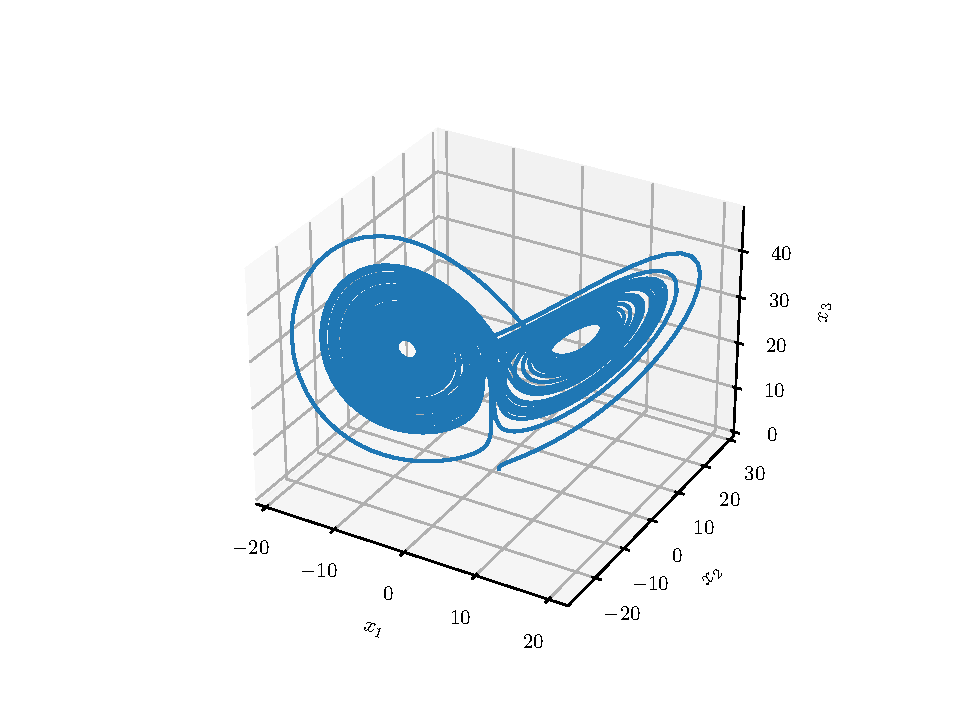
\includegraphics{images/attracteur_lorenz.py.pdf}
\caption{Trajectoire de l'oscillateur de
Lorenz}\label{fig_attracteur_lorenz}
}
\end{figure}

\hypertarget{propriuxe9tuxe9s-asymptotiques}{%
\section{Propriétés
asymptotiques}\label{propriuxe9tuxe9s-asymptotiques}}

Dans la section précédente nous avons répondu à la première question qui
était la sensibilité des solutions aux erreurs de condition initiale et
de modèle. Mais cette étude était en temps fini et nous nous intéressons
maintenant à la seconde question qui est le comportement asymptotique
des solutions. L'étude théorique asymptotique des solutions prend ses
origines dans la thèse de Lyapunov (Lyapunov
\protect\hyperlink{ref-lyap}{1892}). Le but est de rechercher des
critères sur la fonction \(f\) qui nous permettent de prédire ce
comportement~: est-ce que les solutions divergent\,? est-ce qu'elles
tendent vers un point en particulier\,? vers un cycle limite\,?

Dans la suite, pour simplifier, nous étudions les équations
différentielles dites \emph{autonomes}, c'est-à-dire dont la fonction
\(f\) est indépendante du temps. On se donne donc une fonction continue
\(f:X\to \mathbb{R}^n\), avec \(X\) un ouvert de \(\mathbb{R}^n\) et on
prend par défaut \(t_0=0\).

\hypertarget{def_ptEq}{}
\addcontentsline{toc}{subsection}{Point d'équilibre}
\begin{definition}[Point d'équilibre]\label{def_ptEq}
On appelle \emph{point d'équilibre} pour \(f\) (ou pour le système
\(\dot x = f(x)\)) un point \(a\in X\) tel que \[
f(a) = 0  \ .
\] En d'autres termes, la fonction constante égale à \(a\) est alors
solution de \(\dot{x}=f(x)\).
\end{definition}

\hypertarget{ex_pendule}{}
\addcontentsline{toc}{subsubsection}{Pendule}
\begin{exemple}[Pendule]\label{ex_pendule}
L'évolution d'un pendule de longueur \(\ell\) et de masse \(m\) dans le
champ de pesanteur \(g\) peut être décrite par une dynamique du type
\[
\ddot{\theta} = - \frac{\rho}{m} \dot{\theta} -\frac{g}{\ell} \sin\theta 
\] avec \(\rho\geq 0\) un coefficient de frottement. En prenant
\(x=(\theta,\dot{\theta})\), on obtient le système \[
\begin{array}{rcl}
\dot{x}_1 &=& x_2 \\
\dot{x}_2 &=& - \frac{\rho}{m} x_2 -\frac{g}{\ell} \sin x_1
\end{array}
\] Ce système a pour points d'équilibre \((k\pi,0)\),
\(k\in \mathbb{Z}\), qui correspondent soit à la position \emph{basse}
du pendule \(\theta=0\) ou la position \emph{haute} \(\theta=\pi\),
toutes deux à vitesse nulle \(\dot{\theta}=0\). Si le pendule est
initialisé exactement à sa position haute ou basse à vitesse nulle alors
il y reste indéfiniment.
\end{exemple}

\hypertarget{def_attract}{}
\addcontentsline{toc}{subsection}{Attractivité}
\begin{definition}[Attractivité]\label{def_attract}
Un point d'équilibre \(a\) est dit \emph{localement attractif} si
\emph{toutes les solutions maximales initialisées suffisamment proche de
\(a\) sont définies en tout temps positif et convergent vers \(a\)},
c'est-à-dire s'il existe \(\eta>0\) tel que pour tout \(x_0\) vérifiant
\(\|x_0-a\|\leq \eta\), toute solution maximale \(x \in S_f(x_0)\) est
définie sur \(\mathbb{R}_{\geq 0}\) et vérifie \[
\lim_{t\to+\infty} x(t)=a \ .
\] De plus, \(a\) est dit \emph{globalement attractif} si \emph{toutes
les solutions maximales sont définies en tout temps positif et
convergent vers \(a\)}.
\end{definition}

Cette notion intuitive ne dit rien sur le comportement des solutions
pendant le transitoire, c'est-à-dire avant de converger vers \(a\). Des
solutions initialisées proche de \(a\) pourraient s'en éloigner
arbitrairement loin avant de converger, ou mettre un temps
arbitrairement long pour revenir dans un voisinage de \(a\). Pour
garantir une certaine uniformité et robustesse de cette attractivité par
rapport à la condition initiale, on a recours à une notion plus forte
qui est la \emph{stabilité asymptotique}.

\hypertarget{def_stab}{}
\addcontentsline{toc}{subsection}{Stabilité, stabilité asymptotique}
\begin{definition}[Stabilité, stabilité asymptotique]\label{def_stab}
Un point d'équilibre \(a\) est dit:

\begin{itemize}
\item
  \emph{stable} si \emph{les solutions sont définies en tout temps
  positif et restent arbitrairement proche de \(a\) quand elles sont
  initialisées suffisamment proche de \(a\)}, c'est-à-dire pour tout
  \(\varepsilon >0\), il existe \(\eta>0\) tel que pour tout \(x_0\)
  vérifiant \(\|x_0-a\|\leq \eta\), toute solution maximale
  \(x \in S_f(x_0)\) est définie sur \(\mathbb{R}_{\geq 0}\) et vérifie
  \[
  \|x(t)-a\|\leq \varepsilon \quad \forall t\in \mathbb{R}_{\geq 0}\ .
  \]
\item
  \emph{instable} s'il n'est pas stable.
\item
  \emph{localement (resp. globalement) asymptotiquement stable} s'il est
  à la fois stable en plus d'être localement (resp. globalement)
  attractif.
\end{itemize}
\end{definition}

\hypertarget{ex_stab}{}
\addcontentsline{toc}{subsubsection}{Stabilité du pendule}
\begin{exemple}[Stabilité du pendule]\label{ex_stab}
\begin{itemize}
\item
  Lorsqu'un pendule amorti est initialisé arbitrairement proche de sa
  position haute ou dans sa position haute mais à vitesse arbitrairement
  faible, il se met à osciller en passant par sa position basse~:
  l'équilibre haut est donc instable, puisqu'on ne peut pas garder les
  trajectoires dans son voisinage. Par contre, lorsqu'il est initialisé
  proche de sa position basse, il oscille de façon amortie en tendant
  vers l'équilibre bas, qui est donc localement asymptotiquement stable.
  Voir le \protect\hyperlink{fig_pendule}{portrait de phase du pendule
  amorti (Figure~\ref*{fig_pendule}, p. \pageref*{fig_pendule})}.
\item
  Dans le cas d'un pendule non amorti par contre, c'est-à-dire avec
  \(\rho=0\), le pendule oscille indéfiniment à énergie constante~: la
  position basse est alors toujours stable mais plus attractive, et donc
  plus asymptotiquement stable. Voir le
  \protect\hyperlink{fig_pendule}{portrait de phase du pendule non
  amorti (Figure~\ref*{fig_pendule}, p. \pageref*{fig_pendule})}.
\end{itemize}
\end{exemple}

\hypertarget{rem_robustStab}{}
\addcontentsline{toc}{subsection}{Robustesse vis-à-vis des perturbations (pour la culture)}
\begin{remarque}[Robustesse vis-à-vis des perturbations (pour la culture)]\label{rem_robustStab}
L'avantage de la propriété de \emph{stabilité asymptotique} par rapport
à la simple \emph{attractivité} est qu'elle apporte de la robustesse par
rapport aux perturbations. En effet, lorsque qu'un point d'équilibre est
asymptotiquement stable, on peut montrer qu'en présence d'une
perturbation de la dynamique, les solutions restent asymptotiquement
arbitrairement proche de ce point d'équilibre si la perturbation est
suffisamment petite. Il y a donc une sorte de continuité des solutions
par rapport aux perturbations en temps infini (contrairement au résultat
général de continuité par rapport aux conditions initiales qui n'est
qu'en temps fini). Cette propriété n'est pas garantie lorsque le point
d'équilibre n'est qu'attractif et c'est la raison pour laquelle en
pratique, on essaye toujours d'assurer la stabilité asymptotique d'un
système~: on sait alors que même en présence de perturbations
(inévitables en physique), le comportement du système sera proche du
comportement voulu.
\end{remarque}

\hypertarget{Hurwitz}{}
\addcontentsline{toc}{subsection}{Stabilité asymptotique d'un système linéaire stationnaire}
\begin{theoreme}[Stabilité asymptotique d'un système linéaire stationnaire]\label{Hurwitz}
Soit \(A\in \mathbb{R}^{n\times n}\). Le point d'équilibre 0 est
globalement asymptotiquement stable pour le système \[
\dot{x} = Ax
\] si et seulement si les valeurs propres de \(A\) sont toutes à partie
réelle strictement négative. On dit alors que la matrice est de
\emph{Hurwitz}, du nom du mathématicien allemand Adolf Hurwitz.
\end{theoreme}

\hypertarget{duxe9monstration-6}{}
\begin{preuve}\label{duxe9monstration-6}
La notion de \emph{globalement asymptotiquement stable} contient deux
propriétés~: la stabilité et l'attractivité globale. On montrera en
\protect\hyperlink{attrac_stab}{exercice (p. \pageref*{attrac_stab})}
que pour un système linéaire, elles sont équivalentes à l'attractivité
(locale), c'est-à-dire que la stabilité et la globalité viennent
gratuitement. C'est une propriété propre aux systèmes linéaires. Il
suffit donc de trouver un critère caractérisant l'attractivité de 0. On
a vu que les solutions s'écrivent \[
x(t)= e^{At} x_0 \ .
\] Si \(A\) est diagonale, on a \(x_i(t)=e^{\lambda_i t}x_{0,i}\), où
\(\lambda_i\) sont les valeurs propres de \(A\) et l'on voit bien que la
convergence des solutions vers 0 est équivalente à avoir
\(\lambda_i<0\). Maintenant, si \(A\) est diagonalisable, i.e., il
existe \(P\in \mathbb{C}^{n\times n}\) inversible telle que
\(P^{-1} A P\) est diagonale, on a
\(P^{-1} x(t) = e^{P^{-1} A P t} P^{-1} x_0\), et reproduisant le
même argument, \(P^{-1} x\) (et donc \(x\)) converge vers 0 si et
seulement si les entrées diagonales de \(P^{-1} A P\), qui sont les
valeurs propres de \(A\), sont à partie réelle strictement négative.
Ceci dit, toute matrice \(A\) n'est pas diagonalisable. Par contre, il
existe toujours \(P\in \mathbb{C}^{n\times n}\) inversible telle que \[
P^{-1} A P = D + N
\] où \(D\) est diagonale contenant les valeurs propres de \(A\), \(N\)
est nilpotente, c'est-à-dire qu'il existe \(k\in \mathbb{N}\) tel que
\(N^k=0\), et \(D\) et \(N\) commutent. C'est la forme dite \emph{de
Jordan}. Il s'ensuit que \[
P^{-1} e^{At} P = e^{P^{-1} A Pt} = e^{Dt}e^{Nt} = e^{Dt}\sum_{i=0}^k \frac{1}{i!} N^i t^i
\] converge vers zéro si et seulement si, encore, les valeurs propres de
\(A\) sont à partie réelle strictement négative.\hfill$\blacksquare$

Attention ce critère n'est valable que pour \(A\) constant. Le fait que
\(A(t)\) soit de Hurwitz pour tout \(t\) n'implique pas que les
solutions du système \[
\dot{x} = A(t) x 
\] tendent vers 0 ou même restent bornées. Par exemple, la matrice \[
A(t) = \left( \begin{matrix} 
-1+1.5\cos^2t & 1-1.5\sin t \cos t \\
-1-1.5 \sin t \cos t & -1+1.5\sin^2 t
\end{matrix}
\right)
\] a des valeurs propres constantes égales à \(-0.25\pm 0.25\sqrt{7}j\).
Pourtant, \(\dot{x} = A(t) x\) admet des solutions non bornées pour
\(x(0)\) arbitrairement proche de 0.
\end{preuve}

\hypertarget{rem-crit_stabLin}{}
\addcontentsline{toc}{subsection}{Critère de stabilité linéaire (pour la culture)}
\begin{remarque}[Critère de stabilité linéaire (pour la culture)]\label{rem-crit_stabLin}
Notons aussi qu'il existe un critère de \emph{stabilité} pour les
systèmes linéaires autonomes (plus faible que stabilité asymptotique)~:
\(A\) est stable si et seulement si toutes ses valeurs propres sont à
partie réelle négative ou nulle, et toute valeur propre à partie réelle
nulle a ses multiplicités algébriques et géométriques égales.
C'est-à-dire que la dimension du sous-espace propre associé est égale à
sa multiplicité dans le polynôme caractéristique.
\end{remarque}

\hypertarget{crit_stab_dim2}{%
\subsubsection*{\texorpdfstring{Exercice -- Critère de stabilité
asymptotique d'un système linéaire plan
(\(\mathord{\bullet}\))}{Exercice -- Critère de stabilité asymptotique d'un système linéaire plan (•)}}\label{crit_stab_dim2}}

\addcontentsline{toc}{subsubsection}{Critère de stabilité asymptotique d'un système linéaire plan}

Montrer que \(A\in \mathbb{R}^{2\times 2}\) est de Hurwitz si et
seulement si \(\text{tr} A <0\) et \(\text{det} A >0\). Attention, ce
critère ne marche qu'en dimension 2\,!\solref{answer-crit_stab_dim2}

\hypertarget{ressort-1}{%
\subsubsection*{\texorpdfstring{Exercice -- Oscillateurs couplés I
(\(\mathord{\bullet}\))}{Exercice -- Oscillateurs couplés I (•)}}\label{ressort-1}}

\addcontentsline{toc}{subsubsection}{Oscillateurs couplés I}

Considérons deux masses \(m_1,m_2\) évoluant sur un support horizontal,
accrochées entre elles et chacune à un mur via des ressorts de raideur
\(k_1\), \(k_2\), \(k_{12}\). L'évolution de leur position par rapport à
leur position d'équilibre respective est décrite par
\begin{align*}
m_1\ddot{y}_1 &= - \lambda_1 \dot{y}_1 - k_1 y_1 + k_{12} (y_2-y_1) \\
m_2\ddot{y}_2 &= - \lambda_2 \dot{y}_2 - k_2 y_2 - k_{12} (y_2-y_1)
\end{align*} où \(\lambda_1,\lambda_2\) sont des coefficients de
frottement positifs ou nuls. Réduire l'équation différentielle à l'ordre
\(1\), la résoudre et déterminer les points d'équilibre. En supposant
\(m_1=m_2\), \(\lambda_1=\lambda_2\), \(k_1=k_2=k_{12}\), étudier leur
stabilité pour \(\lambda>0\) et \(\lambda = 0\). \emph{On pourra
considérer les nouvelles variables \(y_1+y_2\) et \(y_1-y_2\).}\solref{answer-ressort-1}

\hypertarget{theo_linTangent}{}
\addcontentsline{toc}{subsection}{Lien entre stabilité et stabilité du linéarisé tangent}
\begin{theoreme}[Lien entre stabilité et stabilité du linéarisé tangent]\label{theo_linTangent}
Soit le système défini par \(\dot x = f(x)\) avec
\(f:X \to \mathbb{R}^n\) continûment différentiable et \(a\in X\) un
point d'équilibre.

Si les valeurs propres de la matrice jacobienne \(J_f(a)\) sont toutes à
partie réelle strictement négative (Hurwitz) alors \(a\) est localement
asymptotiquement stable.

Si \(J_f(a)\) a au moins une valeur propre à partie réelle strictement
positive, alors \(a\) est instable.
\end{theoreme}

\hypertarget{duxe9monstration-7}{}
\begin{preuve}\label{duxe9monstration-7}
Pour le premier point, voir la
\protect\hyperlink{lyap-5}{question 5 de l'exercice \emph{Critères de
stabilité de Lyapunov} (p. \pageref*{lyap-5})}, et pour le second, la
\protect\hyperlink{instab-4}{question 4 de l'exercice \emph{Critères
d'instabilité} (p. \pageref*{instab-4})}.\hfill$\blacksquare$
\end{preuve}

Notons cependant que rien ne peut être conclu quant à la stabilité (ou
stabilité asymptotique) de \(a\) si les parties réelles de \(J_f(a)\)
sont négatives ou nulles~: on peut avoir asymptotiquement stable,
seulement stable ou instable. Par exemple, 0 est globalement
asymptotiquement stable pour \(\dot{x} = - x^3\) mais instable pour
\(\dot{x} = x^3\) alors que ces deux dynamiques ont le même linéarisé
(nul) en zéro. Dans ce cas, des critères non linéaires doivent être utilisés (voir les exercices \emph{Critères de stabilité de Lyapunov} (p. \pageref*{lyap-5}) et \emph{Critères d'instabilité} (p. \pageref*{instab-4})).

\hypertarget{ex_pendule_jacob}{}
\addcontentsline{toc}{subsubsection}{Retour au pendule}
\begin{exemple}[Retour au pendule]\label{ex_pendule_jacob}
Reprenons l'\protect\hyperlink{ex_pendule}{exemple du pendule amorti (p.
\pageref*{ex_pendule})}. On a \[
J_f(0,0) = \left( \begin{matrix} 
0 & 1\\
-\frac{g}{\ell} & - \frac{\rho}{m}
\end{matrix}
\right) 
\qquad , \qquad 
J_f(\pi,0)= \left( \begin{matrix} 
0 & 1\\
\frac{g}{\ell} & - \frac{\rho}{m}
\end{matrix}
\right) 
\] Dans le premier cas, \(\text{tr}(J_f(0,0))<0\) et
\(\text{det}(J_f(0,0))>0\). Comme prouvé en
\protect\hyperlink{crit_stab_dim2}{exercice (p.
\pageref*{crit_stab_dim2})}, ceci implique en dimension 2 que
\(J_f(0,0)\) est de Hurwitz. Donc la position basse \((0,0)\) est bien
un équilibre asymptotiquement stable. Dans le deuxième cas par contre,
le produit des valeurs propres
\(\lambda_1\lambda_2 = \text{det}(J_f(\pi,0))<0\). Elles ne peuvent donc
pas être complexes conjuguées et sont nécessairement réelles de signes
opposés. Il s'ensuit que l'une est strictement positive et la position
haute \((\pi,0)\) est donc bien instable.

Notons que si \(\rho=0\), c'est-à-dire que le pendule n'est pas amorti,
les valeurs propres \(J_f(0,0)\) sont imaginaires pures, et l'on ne peut
donc rien conclure quant à la stabilité des points d'équilibre. Une
étude plus approfondie est nécessaire.
\end{exemple}

\hypertarget{asymp_glob-1}{%
\subsubsection*{\texorpdfstring{Exercice -- Stabilité asymptotique I
(\(\mathord{\bullet}\))}{Exercice -- Stabilité asymptotique I (•)}}\label{asymp_glob-1}}

\addcontentsline{toc}{subsubsection}{Stabilité asymptotique I}

Montrer que le point d'équilibre \((0,0)\) est localement
asymptotiquement stable pour le système \[
\begin{array}{rcl}
\dot{x}_1 &=& x_2(1-x_2^2)\\
\dot{x}_2 &=& -(x_1+x_2)(1-x_1^2)
\end{array}
\] L'est-il globalement\,?\solref{answer-asymp_glob-1}

Lorsque le linéarisé ne permet pas de conclure sur la stabilité
asymptotique locale, ou que l'on veut un résultat global, on a recours à
des caractérisations non linéaires, notamment celle de \emph{Lyapunov}
présentée en \protect\hyperlink{exo_lyap}{exercice (p.
\pageref*{exo_lyap})}. Elle consiste à étudier, le long des solutions de
l'équation différentielle, l'évolution d'une quantité positive,
semblable à une énergie, qui s'annule seulement au niveau du point
d'équilibre. En démontrant que cette quantité est conservée, ou mieux,
décroît le long des solutions, on peut typiquement déduire des
propriétés de stabilité ou stabilité asymptotique (potentiellement
globale) du point d'équilibre.

\hypertarget{stab_decroissance}{}
\addcontentsline{toc}{subsection}{Stabilité par décroissance d'une fonction définie positive}
\begin{theoreme}[Stabilité par décroissance d'une fonction définie positive]\label{stab_decroissance}
Soient \(X\) ouvert de \(\mathbb{R}^n\), \(f: X \to \mathbb{R}^n\)
continue, \(a\) un point d'équilibre de \(f\) dans \(X\), \(W\) un
voisinage de \(a\) dans \(X\), et \(V:W\to\mathbb{R}_{\geq 0}\) continue
telle que \[
V(x) > 0 \quad  \forall x\in W\setminus\{a\} \qquad , \qquad V(a)= 0 \ .
\] Si toute solution \(x: I\to \mathbb{R}^n\), \(0\in I\), de
\(\dot x = f(x)\) initialisée dans \(W\) est telle que
\(t\mapsto V(x(t))\) est décroissante sur tout intervalle
\([0,t_1]\subset I\) sur lequel \(x(t)\in W\), alors \(a\) est stable.
\end{theoreme}

\hypertarget{duxe9monstration-8}{}
\begin{preuve}\label{duxe9monstration-8}
Prenons \(\varepsilon>0\) suffisamment petit tel que
\(B_f(a,2\varepsilon)\subset W\). Montrons qu'il existe \(\eta\) tel que
toute solution initialisée dans \(B(a,\eta)\) reste dans
\(B(a,\varepsilon)\subset W\). Tout d'abord, il existe
\(\varepsilon_V>0\) tel que \[
\forall x\in B_f(a,2\varepsilon) \ : \ V(x)\leq \varepsilon_V \ \Longrightarrow x\in B(a,\varepsilon) \ .
\] En effet, sinon, il existerait une suite \((x_k)_{k\in \mathbb{N}}\)
d'éléments de \(B_f(a,2\varepsilon)\) telle que pour tout \(k>0\),
\(V(x_k)\leq \frac{1}{k}\) et \(\|x_k-a\|\geq \varepsilon\). L'ensemble
\(B_f(a,2\varepsilon)\) étant compact, on peut en extraire une
sous-suite convergeant vers \(x^\star\) qui vérifie nécessairement
\(V(x^\star)=0\) par continuité de \(V\) et
\(\|x^\star-a\|\geq \varepsilon\), i.e.~\(x^\star \neq a\). Ceci est
impossible par hypothèse. On a donc l'existence de \(\varepsilon_V\).
Maintenant, par continuité de \(V\) en \(a\) et puisque \(V(a)=0\), il
existe aussi \(\eta>0\) tel que \[
x\in B(a,\eta)  \ \Longrightarrow V(x)\leq \varepsilon_V \ .
\] Finalement, soit une solution maximale \(x\) de \(\dot x = f(x)\)
avec \(x(0)\in B(a,\eta)\). Montrons que \(x(t)\in B(a,\varepsilon)\)
pour tout \(t\geq 0\) où elle est définie. Supposons par l'absurde que
\(x\) sorte de \(B_f(a,2\varepsilon)\), et notons \[
t_1=\inf\{t\geq 0 \ : \ \|x(t)-a\|> 2\varepsilon\} \ ,
\] qui est strictement positif puisque \(\|x(0)-a\|<\eta<\varepsilon\)
et \(x\) est continue. Sur \([0,t_1]\), \(x(t)\in B_f(a,2\varepsilon)\subset W\),
donc par décroissance de \(t\mapsto V(x(t))\) par hypothèse,
\(V(x(t))\leq V(x(0))\leq \varepsilon_V\) et ainsi
\(x(t)\in B(a,\varepsilon)\). En particulier \(\|x(t_1)-a\|<\varepsilon\),
alors que par continuité et définition de \(t_1\),
\(\|x(t_1)-a\| = 2\varepsilon\)~: contradiction. Donc \(x(t)\) reste dans
\(B_f(a,2\varepsilon)\), et le même argument montre alors que
\(x(t)\in B(a,\varepsilon)\subset W\) pour tout \(t\geq 0\) où elle est
définie. Elle reste donc dans un compact de \(X\), et par le
\protect\hyperlink{theo_bouts}{théorème du domaine maximal d'existence
(p. \pageref*{theo_bouts})}, \(x\) est définie sur
\(\mathbb{R}_{\geq 0}\). On obtient la stabilité de
\(a\).\hfill$\blacksquare$
\end{preuve}

\hypertarget{ex_pendule_lyap}{}
\addcontentsline{toc}{subsubsection}{Stabilité du pendule}
\begin{exemple}[Stabilité du pendule]\label{ex_pendule_lyap}
Reprenons le \protect\hyperlink{ex_pendule}{pendule (p.
\pageref*{ex_pendule})} mais cette fois-ci, non amorti, c'est-à-dire
avec \(\rho=0\). Nous n'avons pas pu prouver la stabilité du point
d'équilibre \((0,0)\) par l'étude de la matrice Jacobienne car ses
valeurs propres sont imaginaires pures. Inspirés par la physique,
considérons
\(V:\left] -\pi, \pi\right[\times \mathbb{R}\to \mathbb{R}_{\geq 0}\)
définie par \[
V(x_1,x_2) = \frac{1}{2} m\ell^2 x_2^2 + mg\ell(1-\cos(x_1)) \ .
\] Le premier terme correspond à l'énergie cinétique du pendule, et le
deuxième son énergie potentielle. \(V\) est continue, à valeurs
positives et s'annule seulement en \(x=0\). De plus, pour toute solution
\(t\mapsto x(t)\), \begin{align*}
\frac{d}{dt} V(x(t)) &=  m\ell^2 x_2(t) \dot x_2(t) + mg \ell \sin(x_1(t)) \dot x_1(t) \\
&= m\ell^2 x_2(t)\left(-\frac{g}{\ell} \sin(x_1(t))\right) + mg \ell \sin(x_1(t)) x_2(t) \\
&= 0 
\end{align*} ce qui traduit la conservation de l'énergie en l'absence de
frottement. On en déduit donc la stabilité du point d'équilibre
\((0,0)\).
\end{exemple}

\hypertarget{rem-crit_lyap}{}
\addcontentsline{toc}{subsection}{Fonctions et critères de Lyapunov}
\begin{remarque}[Fonctions et critères de Lyapunov]\label{rem-crit_lyap}
Une telle fonction \(V\) décroissante le long des solutions est appelée
\emph{fonction de Lyapunov}. Comme dans l'exemple précédent, on vérifie
sa décroissance en étudiant le signe, de \[
\frac{d}{dt} V(x(t)) = \langle\nabla V (x(t)), \dot{x}(t)\rangle = \langle\nabla V (x(t)), f(x(t))\rangle \ .
\]
Mais vu que l'on ne sait généralement pas résoudre l'équation
différentielle, on ne connaît pas l'expression de \(x(t)\) et on se
ramène donc à étudier le signe de la quantité
\(\langle\nabla V (x), f(x)\rangle\) pour \(x\in \mathbb{R}^n\) dans un
voisinage de \(a\), ou globalement, par un calcul algébrique sans
considérer les solutions de l'équation différentielle. Ceci débouche sur
les critères de \emph{Lyapunov} présentés en
\protect\hyperlink{exo_lyap}{exercice (p. \pageref*{exo_lyap})}. On peut
se demander s'il existe toujours une telle fonction de Lyapunov, autour
d'un point d'équilibre stable/asymptotiquement stable. La réponse est
oui, mais c'est une question délicate étudiée en détail dans (Bacciotti
and Rosier \protect\hyperlink{ref-BacRos}{2005}).

Au delà de la stabilité donnée par le résultat précédent, les conditions
de Lyapunov permettent aussi de démontrer la stabilité asymptotique
locale du point d'équilibre lorsque l'on a une décroissance
\emph{stricte}, c'est-à-dire lorsque
\(\langle\nabla V (x), f(x)\rangle<0\) pour \(x\neq a\) dans un
voisinage de \(a\). Cette stabilité asymptotique devient \emph{globale}
lorsque cette inégalité est valide globalement et lorsque de plus la
fonction \(V\) est propre, c'est-à-dire si
\(\lim_{\|x\| \to +\infty} V(x) = +\infty\). Attention cette dernière
hypothèse est importante car elle garantit que les solutions restent
bornées et sont bien définies sur \(\mathbb{R}_{\geq 0}\). Sinon on
pourrait avoir des solutions qui explosent en temps fini alors que \(V\)
décroît strictement.

Souvent cependant, la fonction de Lyapunov \(V\) ne décroît pas
\emph{strictement} et ces derniers critères ne s'appliquent pas. On
étudie alors la convergence asymptotique des solutions vers le point
d'équilibre de manière ad-hoc en utilisant une variation très pratique
du fameux \emph{lemme de Barbalat}.
\end{remarque}

\hypertarget{theo_barbalat}{}
\addcontentsline{toc}{subsection}{Lemme de Barbalat}
\begin{theoreme}[Lemme de Barbalat]\label{theo_barbalat}
Soit \(v:[t_0,+\infty[\to \mathbb{R}\) de classe \(C^2\) telle que

\begin{itemize}
\item
  \(\lim_{t\to +\infty} v(t)\) existe et est finie,
\item
  \(\ddot{v}\) est bornée sur \([t_0,+\infty[\).
\end{itemize}

Alors \(\lim_{t\to +\infty} \dot{v}(t) = 0\).
\end{theoreme}

\hypertarget{duxe9monstration-9}{}
\begin{preuve}\label{duxe9monstration-9}
La première hypothèse dit que \(\int_{t_0}^{+\infty} \dot{v}(t)dt\) est
finie et la deuxième implique que \(\dot{v}\) est uniformément continue
sur \([t_0,+\infty[\). Le lemme de Barbalat (dans son énoncé classique)
permet alors de conclure que \(\dot{v}\) converge vers
zéro.\hfill$\blacksquare$

Toujours dans le contexte d'une fonction définie positive décroissante,
et en supposant que \(f\) et \(V\) sont aussi régulières que
nécessaires, on a le fait que \(v(t) = V(x(t))\) décroît, et donc
\(\dot{v}(t)\leq 0\) pour tout \(t\geq 0\). Comme \(v\) est minorée par
0, elle converge asymptotiquement. Si on a par ailleurs démontré la
bornitude des solutions (en temps positif), on a typiquement aussi celle
de leurs dérivées puisque \(\dot{x} = f(x)\), et donc aussi celle de
\(\ddot{v}\). Par Barbalat, on déduit que
\(\dot{v}(t) = \langle\nabla V (x(t)), f(x(t))\rangle\) tend vers 0,
inférant ainsi des propriétés asymptotiques sur les solutions. Par
l'application répétée de Barbalat, on peut arriver à montrer
l'attractivité locale ou globale du point d'équilibre, qui s'ajoute à la
stabilité pour donner sa stabilité asymptotique.
\end{preuve}

\hypertarget{muxe9thode-danalyse-non-linuxe9aire-de-stabilituxe9}{%
\begin{remarque}[M\'ethode non-lin\'eaire d'analyse de stabilit\'e]\label{muxe9thode-danalyse-non-linuxe9aire-de-stabilituxe9}}
La méthode consiste donc à
\begin{itemize}
\item
  chercher une fonction \(V\) définie positive par rapport au point
  d'équilibre qui décroît le long des solutions (on considère souvent
  des sommes de carrés);
\item
  en déduire la stabilité du point d'équilibre par
  \protect\hyperlink{stab_decroissance}{théorème (p.
  \pageref*{stab_decroissance})};
\item
  montrer que les solutions sont bornées en temps positif (par exemple
  en utilisant que \(\lim_{\|x\| \to +\infty} V(x) = +\infty\), voir
  \protect\hyperlink{glob_sol3}{exercice (p. \pageref*{glob_sol3})});
\item
  en déduire par récurrence que toutes les dérivées successives
  nécessaires des solutions sont bornées en utilisant que
  \(\dot{x} = f(x)\) et la régularité de \(f\);
\item
  utiliser le lemme de Barbalat (potentiellement un certain nombre de
  fois sur les dérivées successives) pour montrer que les solutions
  (toutes ou celles dans un voisinage) convergent vers le point
  d'équilibre;
\item
  combiner avec la stabilité pour déduire la stabilité asymptotique
  locale ou globale.
\end{itemize}
\end{remarque}

\hypertarget{ressort-2}{%
\subsubsection*{\texorpdfstring{Exercice -- Oscillateurs couplés II
(\(\mathord{\bullet}\mathord{\bullet}\))}{Exercice -- Oscillateurs couplés II (••)}}\label{ressort-2}}

\addcontentsline{toc}{subsubsection}{Oscillateurs couplés II}

Reprendre l'\protect\hyperlink{ressort-1}{exercice sur les oscillateurs
couplés (p. \pageref*{ressort-1})} et démontrer la stabilité du point
d'équilibre dans le cas général. Montrer que les solutions sont bornées
en temps positif et que le point d'équilibre est globalement
asymptotiquement stable si \(\lambda_1>0\) ou \(\lambda_2>0\). On pourra
pour cela considérer l'énergie mécanique du système.\solref{answer-ressort-2}

\hypertarget{asymp_glob-2}{%
\subsubsection*{\texorpdfstring{Exercice -- Stabilité asymptotique II
(\(\mathord{\bullet}\mathord{\bullet}\))}{Exercice -- Stabilité asymptotique II (••)}}\label{asymp_glob-2}}

\addcontentsline{toc}{subsubsection}{Stabilité asymptotique II}

Montrer que \((0,0)\) est globalement asymptotiquement stable pour \[
\begin{array}{rcl}
\dot{x}_1 &=& x_2\\
\dot{x}_2 &=& -x_1^3-x_2
\end{array}
\] \emph{Indice~: \(x_2^2\) donne de la négativité en \(x_2\), voir
comment compléter avec des termes positifs en \(x_1\)\ldots{}}.\solref{answer-asymp_glob-2}

\hypertarget{exercices-compluxe9mentaires}{%
\chapter{Exercices complémentaires}\label{exercices-compluxe9mentaires}}

En plus des exercices essentiels, les exercices à maîtriser sont marqués
d'une croix (+).

\hypertarget{exo_Torricelli}{%
\section{\texorpdfstring{Ecoulement dans un réservoir
(\(+\))}{Ecoulement dans un réservoir (+)}}\label{exo_Torricelli}}

Considérons un réservoir cylindrique de section \(S\) qui se vide par
une ouverture de section \(s\) située à sa base. On note \(x\) la
hauteur de liquide dans le réservoir. D'après la \emph{loi de
Torricelli}\footnote{Sous l'hypothèse d'incompressibilité du fluide, la
  loi de Bernoulli dit que \[
  p_s + \rho g h_s + \rho \frac{v_s^2}{2}=p_o + \rho g h_o + \rho \frac{v_o^2}{2}
  \] où \(s\) fait référence aux quantités à la surface et \(o\) à
  l'ouverture. On a \(p_s=p_o\) égales à la pression atmosphérique,
  \(h_s-h_o=x\), \(v_s=\frac{s}{S}v_o\) par conservation du débit, et
  \(\dot{x} = - v_s\). On obtient donc \[
  \dot{x} = - \frac{1}{\sqrt{\left(\frac{S}{s}\right)^2-1}} \sqrt{2gx} \approx -\frac{s}{S} \sqrt{2gx}
  \] en supposant que \(s\ll S\).}, l'équation d'évolution de \(x\) est
donnée par \[
\dot{x}=-k\sqrt{|x|} \qquad k = \frac{s}{S}\sqrt{2g}
\] où \(g\) est la pesanteur.

\hypertarget{tor-1}{%
\subsubsection*{Question 1}\label{tor-1}}

\addcontentsline{toc}{subsubsection}{Question 1}

Etant donné un temps initial \(t_0\) et une hauteur initiale
\(x_0\geq 0\), justifier sans calcul que le problème de Cauchy associé
admet des solutions et que les solutions maximales sont définies sur
\(\mathbb{R}\). Que pouvons-nous dire a priori sur l'unicité des
solutions maximales\,?\solref{answer-tor-1}

\hypertarget{tor-2}{%
\subsubsection*{Question 2}\label{tor-2}}

\addcontentsline{toc}{subsubsection}{Question 2}

Pour \((t_0,x_0)\in \mathbb{R}\times \mathbb{R}_{\geq0}\), résoudre le
problème de Cauchy associé.\solref{answer-tor-2}

\hypertarget{tor-3}{%
\subsubsection*{Question 3}\label{tor-3}}

\addcontentsline{toc}{subsubsection}{Question 3}

On qualifie la solution de ``physique'' si elle reste dans
\(\mathbb{R}_{\geq0}\). Commenter l'unicité de la solution physique en
fonction de \(x_0\). Comment pourrait s'interpréter physiquement la
multitude de solutions trouvées\,?\solref{answer-tor-3}

\hypertarget{tor-4}{%
\subsubsection*{Question 4}\label{tor-4}}

\addcontentsline{toc}{subsubsection}{Question 4}

Les solutions sont-elles continues par rapport aux conditions initiales
au sens du \protect\hyperlink{theo_reg_CI}{théorème de régularité des
solutions (p. \pageref*{theo_reg_CI})} donné plus haut\,? Pourquoi\,?\solref{answer-tor-4}

\hypertarget{exo_gronwall}{%
\section{Autour du Lemme de Grönwall}\label{exo_gronwall}}

\hypertarget{gro-1}{%
\subsubsection*{Question 1 (Lemme de Grönwall)}\label{gro-1}}

\addcontentsline{toc}{subsubsection}{Question 1 (Lemme de Grönwall)}

Soient \(I\) un intervalle de \(\mathbb{R}\), \(t_0 \in I\),
\(u,\alpha, \beta : I\to\mathbb{R}_{\geq 0}\) continues, tels que \[
u(t) \leq \alpha(t) + \int_{t_0}^{t}\beta(s) u(s)ds \qquad \forall t\in I \ .
\] Montrer qu'alors \[
u(t) \leq \alpha(t) +  \int_{t_0}^{t} \alpha(s)\beta(s) \exp\left(\int_{s}^t\beta(r)dr \right) ds\qquad \forall t\in I, \ t\geq t_0 \ .
\] En déduire que si \(\alpha\) est constant, \[
u(t) \leq \alpha \exp\left(\int_{t_0}^t\beta(r)dr \right) \qquad \forall t\in I, \ t\geq t_0 \ .
\] \emph{Indice~: poser \(v(t)=\int_{t_0}^t\beta(s)u(s)ds\) et étudier
la dérivée de \(v(t)\exp\left(-\int_{t_0}^t\beta(r)dr\right)\)}.\solref{answer-gro-1}

\hypertarget{gro-2}{%
\subsubsection*{Question 2}\label{gro-2}}

\addcontentsline{toc}{subsubsection}{Question 2}

Utiliser le Lemme de Grönwall pour montrer le
\protect\hyperlink{theo_exist_glob}{théorème d'existence globale de
solutions (p. \pageref*{theo_exist_glob})}.\solref{answer-gro-2}

\hypertarget{gro-3}{%
\subsubsection*{Question 3}\label{gro-3}}

\addcontentsline{toc}{subsubsection}{Question 3}

Utiliser le Lemme de Grönwall pour montrer le
\protect\hyperlink{theo_reg_CI}{théorème de continuité par rapport aux
conditions initiales (p. \pageref*{theo_reg_CI})}. Expliquer pourquoi le
théorème est toujours valable si \(f\) est seulement localement
lipschitzienne par rapport à \(x\) sur \(J\times X\).\solref{answer-gro-3}

\hypertarget{exo_cycle-lim}{%
\section{\texorpdfstring{Cycle limite I
(\(+\))}{Cycle limite I (+)}}\label{exo_cycle-lim}}

Considérons le système \[
\begin{array}{rcl}
\dot{x}_1 &=& x_1+x_2-x_1(x_1^2 + x_2^2)\\
\dot{x}_2 &=& -x_1+x_2-x_2(x_1^2 + x_2^2)
\end{array}
\]

\hypertarget{cycle-lim-1}{%
\subsubsection*{Question 1}\label{cycle-lim-1}}

\addcontentsline{toc}{subsubsection}{Question 1}

Montrer que ce système admet un seul point d'équilibre. Etudier sa
stabilité.\solref{answer-cycle-lim-1}

\hypertarget{cycle-lim-2}{%
\subsubsection*{Question 2}\label{cycle-lim-2}}

\addcontentsline{toc}{subsubsection}{Question 2}

Montrer que quelle que soit la condition initiale, le système admet une
unique solution maximale \(x:I\to \mathbb{R}^2\). Soit
\(V:\mathbb{R}^2\to\mathbb{R}\) définie par
\(V(x) = \|x\|^2 = x_1^2+x_2^2\). En étudiant le signe de
\(\frac{d}{dt}V(x(t))\), montrer que \([t_0,+\infty[ \subset I\).\solref{answer-cycle-lim-2}

\hypertarget{cycle-lim-3}{%
\subsubsection*{Question 3}\label{cycle-lim-3}}

\addcontentsline{toc}{subsubsection}{Question 3}

Montrer que si \(\|x(t_0)\|\neq 1\) alors \(\|x(t)\|\neq 1\) pour tout
\(t\in I\).\solref{answer-cycle-lim-3}

\hypertarget{cycle-lim-4}{%
\subsubsection*{Question 4}\label{cycle-lim-4}}

\addcontentsline{toc}{subsubsection}{Question 4}

En déduire le comportement des solutions en fonction de la condition
initiale.\solref{answer-cycle-lim-4}

\hypertarget{exo_lyap}{%
\section{Critères de stabilité de Lyapunov}\label{exo_lyap}}

Soient \(X\) ouvert de \(\mathbb{R}^n\), \(f: X \to \mathbb{R}^n\)
continue, \(a\) un point d'équilibre de \(f\) dans \(X\), \(W\) un
voisinage de \(a\) dans \(X\), et \(V:W\to\mathbb{R}_{\geq 0}\)
continûment différentiable telle que \[
V(x) > 0 \quad  \forall x\in W\setminus\{a\} \qquad , \qquad V(a)= 0 \ .
\]

\hypertarget{lyap-1}{%
\subsubsection*{Question 1}\label{lyap-1}}

\addcontentsline{toc}{subsubsection}{Question 1}

Montrer que si \(\langle\nabla V (x), f(x)\rangle \leq 0\) pour tout
\(x\in W\) alors \(a\) est stable.\solref{answer-lyap-1}

\hypertarget{lyap-2}{%
\subsubsection*{Question 2}\label{lyap-2}}

\addcontentsline{toc}{subsubsection}{Question 2}

Montrer que si \(\langle \nabla V (x), f(x) \rangle < 0\) pour tout
\(x\in W\setminus \{a\}\) alors \(a\) est localement asymptotiquement
stable.\solref{answer-lyap-2}

\hypertarget{lyap-3}{%
\subsubsection*{Question 3}\label{lyap-3}}

\addcontentsline{toc}{subsubsection}{Question 3}

Montrer que si \(\lim_{\|x\|\to +\infty} V(x) = +\infty\),
\(W=\mathbb{R}^n\), et \(\langle\nabla V (x), f(x)\rangle < 0\) pour
tout \(x\neq a\) alors \(a\) est globalement asymptotiquement stable.\solref{answer-lyap-3}

\hypertarget{lyap-4}{%
\subsubsection*{Question 4 (Application à la stabilité des systèmes
linéaires)}\label{lyap-4}}

\addcontentsline{toc}{subsubsection}{Question 4 (Application à la stabilité des systèmes linéaires)}

Soit \(A\in \mathbb{R}^{n\times n}\) dont les valeurs propres sont
toutes à partie réelle strictement négative, et soit
\(Q\in \mathbb{R}^{n\times n}\) une matrice symétrique définie positive.
Montrer qu'il existe une matrice symétrique définie positive
\(P\in \mathbb{R}^{n\times n}\) telle que \[
A^\top P +P A = - Q \ .
\] \emph{On pourra considérer
\(P=\int_0^{+\infty}\left(e^{As}\right)^\top Q e^{As}ds\).} En déduire
une fonction de Lyapunov pour le système \(\dot{x} = Ax\) et retrouver
que \(0\) est globalement asymptotiquement stable.\solref{answer-lyap-4}

\hypertarget{lyap-5}{%
\subsubsection*{Question 5 (Application à la stabilité via linéarisé
tangent)}\label{lyap-5}}

\addcontentsline{toc}{subsubsection}{Question 5 (Application à la stabilité via linéarisé tangent)}

Soit \(f:X \to \mathbb{R}^n\) continûment différentiable et \(a\in X\)
un point d'équilibre de \(f\) tel que les valeurs propres de la matrice
jacobienne \(J_f(a)\) sont toutes à partie réelle strictement négative.
Montrer que \(a\) est localement asymptotiquement stable pour
\(\dot x = f(x)\), c'est-à-dire démontrer le premier point du
\protect\hyperlink{theo_linTangent}{théorème \emph{Lien entre stabilité
et stabilité du linéarisé tangent} (p. \pageref*{theo_linTangent})}.\solref{answer-lyap-5}

\hypertarget{exo_instab}{%
\section{Critères d'instabilité}\label{exo_instab}}

Soient \(X\) ouvert de \(\mathbb{R}^n\), \(f: X \to \mathbb{R}^n\)
continue et \(a\in X\) un point d'équilibre de \(f\).

\hypertarget{instab-1}{%
\subsubsection*{Question 1 (Théorème de Chetaev)}\label{instab-1}}

\addcontentsline{toc}{subsubsection}{Question 1 (Théorème de Chetaev)}

Soient \(W\) un voisinage de \(a\) dans \(X\) et
\(V:W\to\mathbb{R}\) continûment différentiable telle que \(V(a)=0\) et

\begin{itemize}
\tightlist
\item
  \(V\) prend des valeurs strictement positives arbitrairement près de
  \(a\)~: pour tout \(\eta>0\), il existe \(x\in W\) tel que
  \(\|x-a\|<\eta\) et \(V(x)>0\)~;
\item
  \(\langle\nabla V (x), f(x)\rangle > 0\) pour tout \(x\in W\) tel que
  \(V(x)>0\).
\end{itemize}

Montrer que \(a\) est instable. On remarquera que, contrairement aux
critères de stabilité, \(V\) n'est pas supposée positive.\solref{answer-instab-1}

\hypertarget{instab-2}{%
\subsubsection*{Question 2 (Exemples)}\label{instab-2}}

\addcontentsline{toc}{subsubsection}{Question 2 (Exemples)}

Montrer que \(0\) est instable pour \(\dot{x} = x^3\) sur \(\mathbb{R}\),
puis pour le système \[
\dot{x}_1 = x_1 \qquad , \qquad \dot{x}_2 = -x_2
\] sur \(\mathbb{R}^2\). \emph{On pourra chercher \(V\) sous la forme
d'une forme quadratique.}\solref{answer-instab-2}

\hypertarget{instab-3}{%
\subsubsection*{Question 3 (Application à l'instabilité des systèmes
linéaires (\(\mathord{\bullet}\mathord{\bullet}\)))}\label{instab-3}}

\addcontentsline{toc}{subsubsection}{Question 3 (Application à l'instabilité des systèmes linéaires)}

Soit \(A\in \mathbb{R}^{n\times n}\) ayant au moins une valeur propre à
partie réelle strictement positive. Montrer qu'il existe \(\sigma>0\),
une matrice symétrique définie positive \(Q\in \mathbb{R}^{n\times n}\)
et une matrice symétrique \(P\in \mathbb{R}^{n\times n}\) vérifiant
\(\bar{x}^\top P \bar{x}>0\) pour au moins un \(\bar{x}\in\mathbb{R}^n\),
telles que \[
A^\top P + PA = 2\sigma P + Q \ .
\] En déduire que \(0\) est instable pour
\(\dot{x}=Ax\).\solref{answer-instab-3}

\hypertarget{instab-4}{%
\subsubsection*{Question 4 (Application à l'instabilité via linéarisé
tangent)}\label{instab-4}}

\addcontentsline{toc}{subsubsection}{Question 4 (Application à l'instabilité via linéarisé tangent)}

Soit \(f:X \to \mathbb{R}^n\) continûment différentiable et \(a\in X\)
un point d'équilibre de \(f\) tel que la matrice jacobienne \(J_f(a)\) a
au moins une valeur propre à partie réelle strictement positive. Montrer
que \(a\) est instable pour \(\dot x = f(x)\), c'est-à-dire démontrer le
second point du \protect\hyperlink{theo_linTangent}{théorème \emph{Lien
entre stabilité et stabilité du linéarisé tangent} (p.
\pageref*{theo_linTangent})}.\solref{answer-instab-4}

\hypertarget{exo_cycle-lim-volterra}{%
\section{\texorpdfstring{Cycle limite II
(\(+\))}{Cycle limite II (+)}}\label{exo_cycle-lim-volterra}}

Les équations de Lotka-Volterra, ou ``modèle proie-prédateur'', sont
couramment utilisées pour décrire la dynamique de systèmes biologiques
dans lesquels un prédateur et sa proie interagissent dans un milieu
commun. Elles ont été proposées indépendamment par A. J. Lotka en 1925
et V. Volterra en 1926 et s'écrivent de la manière suivante~:
\begin{align*}
\dot{x}_1 &= x_1(\alpha -\beta x_2) \\
\dot{x}_2 &= -x_2(\gamma - \delta x_1)
\end{align*} où \(x_1\) et \(x_2\) désignent le nombre (positif) de
proies et de prédateurs respectivement et \(\alpha\), \(\beta\),
\(\gamma\), \(\delta\) sont des paramètres strictement positifs.

\hypertarget{cycle-lim-volterra-1}{%
\subsubsection*{Question 1}\label{cycle-lim-volterra-1}}

\addcontentsline{toc}{subsubsection}{Question 1}

Donner une interprétation physique à chaque terme de la dynamique.
Montrer qu'il existe deux points d'équilibre \((0,0)\) et
\(\bar{x}\in \mathbb{R}_{> 0}\times\mathbb{R}_{> 0}\). Que peut-on dire
de leur stabilité à ce stade\,?\solref{answer-cycle-lim-volterra-1}

\hypertarget{cycle-lim-volterra-2}{%
\subsubsection*{Question 2}\label{cycle-lim-volterra-2}}

\addcontentsline{toc}{subsubsection}{Question 2}

Démontrer que toute solution initialisée dans
\(\mathbb{R}_{> 0}\times\mathbb{R}_{> 0}\) reste dans
\(\mathbb{R}_{> 0}\times\mathbb{R}_{> 0}\) sur son ensemble de
définition.\solref{answer-cycle-lim-volterra-2}

\hypertarget{cycle-lim-volterra-3}{%
\subsubsection*{Question 3}\label{cycle-lim-volterra-3}}

\addcontentsline{toc}{subsubsection}{Question 3}

On considère la fonction \[
H(x_1,x_2) = \delta x_1 - \gamma \ln x_1 + \beta x_2 - \alpha \ln x_2  
\] définie sur \(\mathbb{R}_{> 0}\times \mathbb{R}_{> 0}\). Calculer la
dérivée de \(H\) le long des solutions initialisées dans
\(\mathbb{R}_{> 0}\times \mathbb{R}_{> 0}\). En déduire que toute
solution maximale initialisée dans
\(\mathbb{R}_{> 0}\times \mathbb{R}_{> 0}\) est définie sur
\(\mathbb{R}\).\solref{answer-cycle-lim-volterra-3}

\hypertarget{cycle-lim-volterra-4}{%
\subsubsection*{Question 4}\label{cycle-lim-volterra-4}}

\addcontentsline{toc}{subsubsection}{Question 4}

La figure ci-dessous représente les courbes de niveau de \(H\). Où se
trouve \(\bar{x}\)\,? Qu'en conclut-on sur le comportement des
solutions\,? En déduire que \(\bar{x}\) est stable, au sens de la
définition de stabilité.\solref{answer-cycle-lim-volterra-4}

\begin{figure}
	\hypertarget{fig_cycle_limiteII_courbes}{%
		\centering
		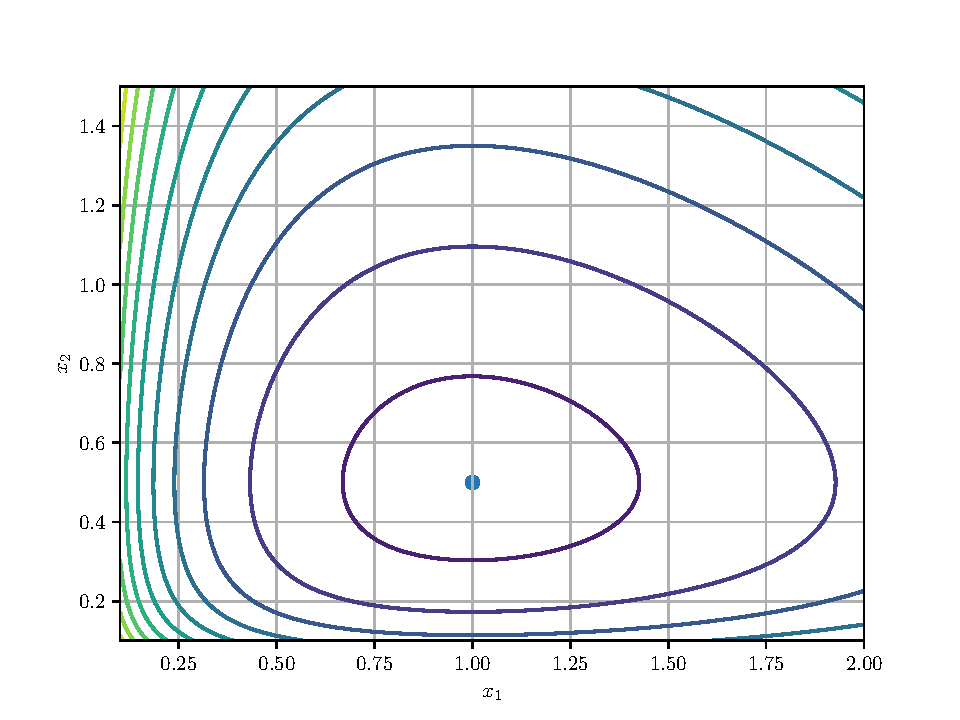
\includegraphics{images/cycle_limiteII_courbes.py.pdf}
		\caption{Courbes de niveau de \(H\) dans l'exercice Cycle Limite
			II}\label{fig_cycle_limiteII_courbes}
	}
\end{figure}

Imaginons maintenant que l'on ait moyen de jouer sur la vitesse de
reproduction des prédateurs, i.e., le système évolue selon
\begin{align*}
\dot{x}_1 &= x_1(\alpha -\beta x_2) \\
\dot{x}_2 &= -x_2(\gamma - \delta x_1) + u(t)
\end{align*} où l'on peut choisir \(t\mapsto u(t)\) librement. On
souhaite stabiliser la population de proie \(x_1\) à une valeur
\(x_1^*>0\).

\hypertarget{cycle-lim-volterra-5}{%
\subsubsection*{Question 5}\label{cycle-lim-volterra-5}}

\addcontentsline{toc}{subsubsection}{Question 5}

Quelles doivent être les valeurs de \(x_2\) et \(u\) à l'équilibre\,?\solref{answer-cycle-lim-volterra-5}

\hypertarget{cycle-lim-volterra-6}{%
\subsubsection*{Question 6}\label{cycle-lim-volterra-6}}

\addcontentsline{toc}{subsubsection}{Question 6}

Justifier que l'on veuille faire suivre à \(x_2\) la référence
\(v_r(x_1) = \frac{\alpha}{\beta} + \lambda_1 (x_1-x_1^*)\) avec
\(\lambda_1>0\). En utilisant la fonction de Lyapunov \[
V(x_1,x_2) = (x_1-x_1^*)^2 + (x_2-v_r(x_1))^2
\] et en supposant que \(x\) est mesuré en temps réel, proposer une loi
de contrôle \(t\mapsto u(t)\) qui stabilise asymptotiquement
\((x_1^*,x_2^*)\), au moins localement.\solref{answer-cycle-lim-volterra-6}

\hypertarget{attrac_stab}{%
\section{Attractivité locale implique stabilité asymptotique globale
pour un système linéaire}\label{attrac_stab}}

Soit \(A\in \mathbb{R}^{n\times n}\). Montrer que si 0 est localement
attractif pour $\dot{x} = Ax$ alors il l'est globalement et 0 est stable.\solref{answer-attrac_stab}

\hypertarget{exo_cont_lin}{%
\section{Stabilisation d'une chaîne
d'intégrateurs}\label{exo_cont_lin}}

Considérons un système du type \[
\begin{array}{rcl}
\dot{x}_1 &=& x_2 \\
\dot{x}_2 &=& x_3 \\
&\vdots&\\
\dot{x}_{n-1} &=& x_n \\
\dot{x}_n &=& \phi(x) + u(t)
\end{array}
\] avec \(\phi:\mathbb{R}^n \to \mathbb{R}\) continue et
\(u:\mathbb{R}\to \mathbb{R}\) une entrée. On aimerait choisir \(u\)
pour rendre un point \(x^*\in \mathbb{R}^n\) globalement
asymptotiquement stable.

\hypertarget{cont-lin-1}{%
\subsubsection*{Question 1}\label{cont-lin-1}}

\addcontentsline{toc}{subsubsection}{Question 1}

Que doit vérifier \(x^*\) pour qu'il puisse être un point d'équilibre\,?
Quelle est la commande \(u^*\) associée\,?\solref{answer-cont-lin-1}

\hypertarget{cont-lin-2}{%
\subsubsection*{Question 2}\label{cont-lin-2}}

\addcontentsline{toc}{subsubsection}{Question 2}

Si on mesure \(t\mapsto x(t)\), montrer que l'on peut alors toujours
choisir \(t\mapsto u(t)\) pour rendre \(x^*\) globalement
asymptotiquement stable.\solref{answer-cont-lin-2}

\hypertarget{cont-lin-3}{%
\subsubsection*{Question 3}\label{cont-lin-3}}

\addcontentsline{toc}{subsubsection}{Question 3}

Comment faire si l'on veut maintenant faire suivre au système une
trajectoire de référence \(t\mapsto x_r(t)\)\,?\solref{answer-cont-lin-3}

\hypertarget{exo_kepler}{%
\section{\texorpdfstring{Problème de Kepler~: collision, libération et
orbites circulaires
(\(\mathord{\bullet}\mathord{\bullet}\))}{Problème de Kepler : collision, libération et orbites circulaires (••)}}\label{exo_kepler}}

On s'intéresse au mouvement d'un satellite (ou d'une planète) de masse
négligeable attiré par un corps ponctuel de masse \(M\) placé à
l'origine. En notant \(q\in \mathbb{R}^3\) la position du satellite et
\(\mu = G M>0\), avec \(G\) la constante de gravitation, la loi de la
gravitation universelle donne \[
\ddot{q} = -\mu \frac{q}{\|q\|^3} \ .
\] Résoudre cette équation (le \emph{problème de Kepler}) permet
d'établir les lois de Kepler. On se propose ici d'obtenir, \emph{sans la
résoudre}, des propriétés qualitatives fortes de ses solutions à l'aide
des outils du cours. On écrit l'équation sous la forme d'un système du
premier ordre en posant \(v=\dot q\) et \(x=(q,v)\), défini sur l'ouvert
\(X = \left(\mathbb{R}^3\setminus\{0\}\right)\times \mathbb{R}^3\). Pour
une solution \(t\mapsto (q(t),v(t))\), on note \[
E = \frac{1}{2}\|v\|^2 - \frac{\mu}{\|q\|} \qquad , \qquad L = q\times v
\] respectivement l'\emph{énergie} (par unité de masse) et le
\emph{moment cinétique} (par unité de masse), où \(\times\) désigne le
produit vectoriel.

\hypertarget{kepler-1}{%
\subsubsection*{Question 1 (Cadre)}\label{kepler-1}}

\addcontentsline{toc}{subsubsection}{Question 1 (Cadre)}

Montrer que pour toute condition initiale \((q_0,v_0)\in X\), le
problème de Cauchy admet une unique solution maximale
\((q,v):\left]\tmin,\tmax\right[\to X\). Montrer que \(E\) et \(L\) sont
constants le long des solutions. Que dit le
\protect\hyperlink{theo_bouts}{théorème du domaine maximal d'existence
(p. \pageref*{theo_bouts})} si \(\tmax<+\infty\)\,? Interpréter
physiquement les deux alternatives.\solref{answer-kepler-1}

\hypertarget{kepler-2}{%
\subsubsection*{Question 2 (Confinement et vitesse de
libération)}\label{kepler-2}}

\addcontentsline{toc}{subsubsection}{Question 2 (Confinement et vitesse de libération)}

Montrer l'\emph{identité de Lagrange-Jacobi} \[
\frac{d^2}{dt^2}\left(\frac{\|q(t)\|^2}{2}\right) = 2E + \frac{\mu}{\|q(t)\|} \ .
\] En déduire que

\begin{itemize}
\tightlist
\item
  si \(E<0\), alors \(\|q(t)\|\leq \frac{\mu}{|E|}\) pour tout
  \(t\in\left]\tmin,\tmax\right[\) (le satellite reste confiné)~;
\item
  si \(E>0\) et \(\tmax=+\infty\), alors
  \(\lim_{t\to+\infty}\|q(t)\|=+\infty\) (le satellite s'échappe).
\end{itemize}

Quelle condition sur la vitesse initiale \(\|v_0\|\) garantit
\(E>0\)\,? Cette vitesse est appelée \emph{vitesse de libération}.\solref{answer-kepler-2}

\hypertarget{kepler-3}{%
\subsubsection*{Question 3 (Pas de collision si \texorpdfstring{\(L\neq
0\)}{L non nul})}\label{kepler-3}}

\addcontentsline{toc}{subsubsection}{Question 3 (Pas de collision si L non nul)}

Montrer que \(\|L\|\leq \|q\|\,\|v\|\) et en déduire que pour tout
\(t\in\left]\tmin,\tmax\right[\), \[
\|L\|^2 \leq 2E\|q(t)\|^2 + 2\mu \|q(t)\| \ .
\] On suppose \(L\neq 0\). Montrer qu'il existe \(r_{\min}>0\) tel que
\(\|q(t)\|\geq r_{\min}\) pour tout \(t\). En déduire que \(v\) est
bornée, puis que la solution est globale, i.e. \(\tmin=-\infty\) et
\(\tmax=+\infty\).\solref{answer-kepler-3}

\hypertarget{kepler-4}{%
\subsubsection*{Question 4 (Collision en temps fini si
\texorpdfstring{\(L=0\)}{L nul})}\label{kepler-4}}

\addcontentsline{toc}{subsubsection}{Question 4 (Collision en temps fini si L nul)}

On suppose maintenant \(L=0\) et on note \(u = q_0/\|q_0\|\).

\begin{enumerate}
\def\labelenumi{\alph{enumi})}
\tightlist
\item
  Montrer que \(t\mapsto \frac{q(t)}{\|q(t)\|}\) est constante, et donc
  que \(q(t) = r(t)\, u\) avec \(r(t)=\|q(t)\|>0\). Montrer que \(r\)
  vérifie \[
  \ddot{r} = -\frac{\mu}{r^2} \ .
  \]
\item
  On suppose de plus \(E<0\). Montrer que \(\tmax<+\infty\) et que
  \(\lim_{t\to\tmax}\|q(t)\| = 0\)~: le satellite percute le corps
  central en temps fini. \emph{Indice~: raisonner par l'absurde en
  supposant \(\tmax=+\infty\), distinguer selon le signe de \(\dot r\),
  et utiliser le \protect\hyperlink{theo_barbalat}{Lemme de Barbalat
  (p. \pageref*{theo_barbalat})}.}
\end{enumerate}\solref{answer-kepler-4}

\hypertarget{kepler-5}{%
\subsubsection*{Question 5 (Stabilité des orbites
circulaires)}\label{kepler-5}}

\addcontentsline{toc}{subsubsection}{Question 5 (Stabilité des orbites circulaires)}

On suppose à nouveau \(L\neq 0\) et on note \(\ell=\|L\|\) et
\(r(t)=\|q(t)\|\).

\begin{enumerate}
\def\labelenumi{\alph{enumi})}
\tightlist
\item
  Montrer l'identité \(\|q\times v\|^2 = \|q\|^2\|v\|^2 - (q\cdot v)^2\)
  et en déduire que \(r\) est solution de l'équation différentielle
  \emph{autonome} \[
  \ddot{r} = \frac{\ell^2}{r^3} - \frac{\mu}{r^2}
  \] sur \(\mathbb{R}_{>0}\).
\item
  Montrer que le système d'état \((r,\dot r)\) associé admet un unique
  point d'équilibre \((r^*,0)\), que l'on exprimera en fonction de
  \(\ell\) et \(\mu\). A quel mouvement du satellite correspond-il\,?
\item
  Montrer que le théorème du linéarisé tangent ne permet pas de conclure
  quant à la stabilité de cet équilibre.
\item
  Exprimer \(E\) en fonction de \(r\) et \(\dot r\) et en déduire une
  fonction définie positive permettant de montrer que \((r^*,0)\) est
  stable. Est-il asymptotiquement stable\,? Interpréter.
\item
  Pourquoi ne peut-on pas parler de stabilité de l'orbite circulaire
  pour le système complet d'état \((q,v)\) avec les définitions du
  cours\,?
\end{enumerate}\solref{answer-kepler-5}

\hypertarget{annexes}{%
\chapter{Annexes}\label{annexes}}

\hypertarget{app_peano}{%
\section{Preuve du théorème de Peano-Arzelà
(Hors-programme)}\label{app_peano}}

Cette preuve repose sur le théorème d'Ascoli~:

\begin{quote}
Soient \(K\) un espace métrique compact, \(Y\) un espace métrique
complet, et \(S\subset C(K,Y)\), où \(C(K,Y)\) est l'ensemble des
fonctions continues de \(K\) dans \(Y\). Les deux propriétés suivantes
sont équivalentes~:

\begin{enumerate}
\def\labelenumi{\arabic{enumi}.}
\item
  \(S\) est \emph{relativement compact} dans \(C(K,Y)\)
\item
  \(S\) est \emph{équicontinu} et pour tout \(z\in K\),
  \(\{g(z) \ , \ g\in S \}\) est \emph{relativement compacte} dans
  \(Y\).
\end{enumerate}
\end{quote}

On dit qu'un ensemble est \emph{relativement compact} si son adhérence
est compacte. En dimension finie, vu que ``compact'' est équivalent à
``fermé-borné'' et que l'adhérence est fermée par définition,
``relativement compact'' est équivalent à ``borné''. Mais ce n'est pas
le cas en dimension infinie (en particulier \(C(K,Y)\)) où
``relativement compact'' est alors équivalent au fait de pouvoir
extraire des suites convergentes dans l'adhérence de l'ensemble.

Ici, puisque \(K\) est compact et \(Y\) complet, on peut montrer que
\(C(K,Y)\) muni de la norme uniforme \(\|\cdot\|_\infty\) est complet,
donc fermé. Il s'ensuit que ``\(S\) est relativement compact dans
\(C(K,Y)\)'' implique pouvoir extraire de toute suite de \(S\) une
sous-suite convergente dans \(C(K,Y)\) (au sens de
\(\|\cdot\|_\infty\)). C'est ce que nous allons utiliser pour prouver
l'existence d'une solution au problème de Cauchy.

Maintenant, le deuxième terme nécessitant des explications est
l'\emph{équicontinuité} de \(S\). Cette notion veut simplement dire que
les fonctions dans \(S\) sont toutes continues \emph{au même rythme},
i.e., plus précisément, \[
\forall \varepsilon >0 \ \exists \delta \ , \quad \ d_K(z_a,z_b)\leq \delta \; \Longrightarrow \;\forall g\in S \ , \  d_Y(g(z_a),g(z_b)) \leq \varepsilon \ ,
\] où \(d_K\) et \(d_Y\) sont les distances sur \(K\) et \(Y\)
respectivement.

Revenons maintenant à nos moutons. On suppose donc \(f\) continue sur
\(J\times X\) et on veut montrer que \(S_f(t_0,x_0)\neq \emptyset\).
Soient d'abord \(\tau >0\) et \(r>0\), tels que
\(\mathcal{C}:= [t_0-\tau,t_0+\tau]\times B_f(x_0,r) \subset J\times X\).
Soit \(\tau_m\in]0, \tau]\) tel que
\(\tau_m\max_\mathcal{C}\|f\|\leq r\). On va montrer l'existence d'une
solution définie par sa forme intégrale \[
x(t) = x_0 + \int_{t_0}^t f(s,x(s)) ds
\] sur \([t_0,t_0+\tau_m]\) et la preuve sur \([t_0-\tau_m,t_0]\) se
fait de la même façon.

L'idée est d'approximer de plus en plus finement la forme intégrale et
montrer que ce procédé converge. On définit donc pour
\(\epsilon \in ]0,1[\) la fonction \begin{align*}
x_\epsilon(t) &= x_0 & \forall t\in [t_0-1,t_0] \\
&= x_0 + \int_{t_0}^t f(s,x_\epsilon(s-\epsilon)) ds & \forall t\in [t_0,t_0+\tau_m]
\end{align*} Ces fonctions sont définies et continues sur
\([t_0-1,t_0]\). Puis sur \([t_0,t_0+\epsilon]\cap[t_0,t_0+\tau_m]\), on
voit que l'intégrale ne dépend que de \(x_\epsilon\) sur
\([t_0-1,t_0]\), donc elle est toujours bien définie et continue. De
proche en proche, \(x_\epsilon\) est donc bien définie et continue sur
\([t_0-1,t_0+\tau_m]\). En fait, \(\epsilon\) représente un petit retard
introduit dans l'intégrale pour la rendre explicite. Si l'on arrive à
montrer que ces fonctions convergent vers une fonction continue lorsque
\(\epsilon\) tend vers 0, cette limite sera solution de l'équation
intégrale sur \([t_0,t_0+\tau_m]\) et sera donc solution.

La première étape est de montrer de proche en proche, grâce au retard,
que \(x_\epsilon(t)\in B_f(x_0,r)\) pour tout
\(t\in [t_0-1,t_0+\tau_m]\) puisque
\(\tau_m\max_\mathcal{C}\|f\|\leq r\). Donc \[
\forall \epsilon \in ]0,1[ \ , \ x_\epsilon \in E:=C([t_0-1,t_0+\tau_m],B_f(x_0,r)) \ .
\] De plus, pour tout \(\epsilon \in ]0,1[\) et pour tout
\((t,t')\in [t_0-1,t_0+\tau_m]^2\), \[
\|x_\epsilon(t) - x_\epsilon(t') \| \leq \max_\mathcal{C}\|f\| \, |t-t'|
\] donc la famille \(S:=\{x_\epsilon , \ \epsilon \in ]0,1[ \}\) est
équicontinue. De plus, vu que leur image est bornée dans \(B_f(x_0,r)\)
de dimension finie, elle est bien relativement compacte. Le
théorème d'Ascoli nous dit alors que \(S\) est relativement compacte
dans \(E\). Il existe donc une sous suite \(x_{\epsilon_k}\) telle que
\(\lim_{k\to +\infty} \epsilon_k =0\) et
\(\lim_{k\to +\infty} x_{\epsilon_k} = x^\star \in E\) au sens de la
norme uniforme \(\|\cdot \|\). Par uniforme continuité de \(f\) sur le
compact \(\mathcal{C}\), on en déduit alors que pour tout
\(s\in [t_0,t_0+\tau_m]\),
\(\lim_{k\to +\infty} f(s,x_{\epsilon_k}(s-\epsilon_k))= f(s,x^\star(s))\)
et donc que \(x^\star\) est bien solution de l'équation intégrale, ce
qui donne le résultat.

\hypertarget{pr_theo_bouts}{%
\section{Preuve du théorème du domaine maximal
d'existence}\label{pr_theo_bouts}}

Soit \(x: I \to \mathbb{R}^n\) une solution dans \(S_f(t_0,x_0)\). Si
\(x\) n'est pas une solution maximale, elle peut être prolongée sur un
intervalle \(I'\) contenant strictement \(I\) par définition, donc on
peut supposer sans perte de généralité que \(I\) est fermé d'un côté,
disons à droite, et nous allons montrer qu'elle peut être prolongée sur
un intervalle maximal d'existence à droite. Si elle peut être prolongée
sur \([t_0,+\infty)\), c'est directement un intervalle maximal à droite
et donc on suppose que \(x\) est définie sur \([t_0,t_1]\) et ne peut
être prolongée sur \([t_0,+\infty)\). La preuve de ce qu'il se passe à
gauche de \(t_0\) est similaire.

Soit \(K\) un compact de \(J\times X\) contenant \(x(t)\) pour
\(t\in [t_0,t_1]\) (qui existe par continuité de \(x\) sur le compact
\([t_0,t_1]\)). Comme \(J\times X\) est ouvert, il existe \(\tau,r\)
strictement positifs tels que \[
\mathcal{C}:= \bigcup_{(t_{\rm init},x_{\rm init})\in K} [t_{\rm init}-\tau,t_{\rm init}+\tau] \times B_f(x_{\rm init},r) \subset J\times X \ .
\] \(\mathcal{C}\) est compact et \(f\) continue sur \(\mathcal{C}\)
donc il existe \(0<\tau_m<\tau\) tel que
\(\tau_m \max_\mathcal{C}\|f\| \leq r\). En reproduisant la preuve du
théorème de Peano-Arzelà, on voit que pour toute condition initiale
\((t_{\rm init},x_{\rm init})\) dans \(K\), il existe une solution au
problème de Cauchy définie au moins sur
\([t_{\rm init}-\tau_m,t_{\rm init}+\tau_m]\).

Revenons donc à notre solution \(x\) définie sur \([t_0,t_1]\) dans
\(K\). Dénotant \(x_1:= x(t_1)\), on a \((t_1,x_1)\in K\) donc il existe
\(x' : [t_1-\tau_m,t_1+\tau_m] \to \mathbb{R}^n\) dans \(S_f(t_1,x_1)\).
Alors on peut construire
\(\tilde{x}: [t_0,t_1+\tau_m] \to \mathbb{R}^n\) telle que \[
\tilde{x}(t) = 
\left\{
\begin{array}{ll}
x(t) & \text{si } t\in [t_0,t_1] \\
x'(t) & \text{si } t>t_1
\end{array}
\right.
\] \(\tilde{x}\) est bien continue et à valeurs dans \(J\times X\) sur
\([t_0,t_1+\tau_m]\). De plus, elle est de classe \(C^1\) sur
\(]t_0,t_1+\tau_m[\setminus \{ t_1\}\) telle que
\(\dot{\tilde{x}}(t) = f(t,\tilde{x}(t))\) pour tout
\(t\in ]t_0,t_1+\tau_m[\setminus \{ t_1\}\). Par continuité de
\(\tilde{x}\) en \(t_1\) et de \(f\) en \((t_1,x_1)\), on en déduit que
\(\tilde{x}\) est bien \(C^1\) sur \(]t_0,t_1+\tau_m[\). Donc
\(\tilde{x}\in S_f(t_0,x_0)\). On a donc trouvé une prolongation
\(\tilde{x}\) de la solution \(x\) sur l'intervalle
\([t_0,t_1+\tau_m]\). Si \((t_1+\tau_m,\tilde{x}(t_1+\tau_m))\) est
toujours dans \(K\), on peut itérer le processus. Parce que \(\tau_m\)
est uniforme sur \(K\) et \(K\) est compact, on construit ainsi en un
nombre fini d'itérations une extension \(\tilde{x}\) de \(x\) qui va
finir par sortir de \(K\), c'est-à-dire, définie sur \([t_0,t_K]\) avec
\(t_K>t_1\) tel que \((t_K,\tilde{x}(t_K))\notin K\).

Considérons maintenant une suite strictement croissante de compacts
\((K_n)\) de \(J\times X\), avec \(K_0=K\), telle que pour tout \(n\),
\(K_n \subset \mathring{K}_{n+1}\) et
\(\cup_n \mathring{K}_{n} = J\times X\). Pour chaque \(n\),
on construit récursivement une extension \(\tilde{x}\) de \(x\) sur des
intervalles de plus en plus grand \([t_0,t_{K_n}]\) tels que
\((t_{K_n},\tilde{x}(t_{K_n})) \notin K_n\). Puisqu'on a supposé que
\(x\) n'était pas prolongeable sur \([t_0,+\infty[\), la suite des
\((t_{K_n})\) est strictement croissante, bornée, et on peut donc en
extraire une sous-suite qui converge. On note \(\tmax\) cette limite. On
a donc construit une prolongation \(\tilde{x}\) de \(x\) définie sur
\([t_0,\tmax)\). De plus, par croissance des \(K_n\), la suite des
\((t_{K_n},\tilde{x}(t_{K_n})) \notin K_n\) sort définitivement de
chacun des \(K_n\) et donc devient ``de plus en plus grand'\,'. Ou bien
\((\tilde{x}(t_{K_n}))\) est non-bornée, ou bien
\((\tilde{x}(t_{K_n}))\) est bornée, et on peut en extraire une
sous-suite qui converge disons vers \(x^*\), qui est dans la frontière
de \(J\times X\). Donc dans les deux cas, \(x\) ne peut pas être
prolongée à droite au delà de \(\tmax\). On a donc bien prolongé \(x\)
en une solution maximale à droite. On fait de même à gauche.

Maintenant, considérons une solution maximale \(x: I \to \mathbb{R}^n\)
dans \(S_f(t_0,x_0)\). Alors \(I\) est ouvert, de la forme
\(]\tmin,\tmax[\) avec \(\tmin,\tmax\) dans
\(\mathbb{R}\cup \{+\infty,-\infty\}\), car sinon, on pourrait prolonger
\(x\) de la même manière que plus haut sur un intervalle strictement
plus grand.

Supposons \(\tmax\) fini. Montrons qu'alors
\(\|x(t)\| + 1/d\big((t,x(t)),\partial (J\times X)\big)\) tend vers
\(+\infty\) lorsque \(t\) tend vers \(\tmax\). La propriété se montre de
manière similaire en \(\tmin\). Pour cela, nous allons montrer que
lorsque \(t\) se rapproche de \(\tmax\), \((t,x(t))\) finit par sortir
définitivement de tout sous-ensemble \(K\) compact de \(J\times X\).
Cela suffit~: pour \(M>0\), l'ensemble \[
K_M = \Big\{(t,x)\in J\times X \ : \ t\leq \tmax \ , \ \|x\|\leq M \ , \ d\big((t,x),\partial (J\times X)\big)\geq \frac{1}{M}\Big\}
\] est borné, et fermé dans \(\mathbb{R}\times\mathbb{R}^n\) (un point
limite de \(J\times X\) à distance au moins \(1/M\) de la frontière est
dans \(J\times X\)), donc compact~; si \((t,x(t))\) en sort
définitivement, alors \(\|x(t)\| + 1/d > M\) pour \(t\) proche de
\(\tmax\), et ce pour tout \(M\). Soit donc \(K\) compact de
\(J\times X\).

Supposons d'abord qu'il existe \(\tau\) tel que \((t,x(t))\in K\) pour
tout \(t\in [\tau,\tmax[\). Puisque \(f\) est continue, \(\|f(t,x)\|\)
est borné disons par \(M\) sur \(K\). Donc pour toute suite \((t_k)\)
d'éléments de \([\tau,\tmax[\) tendant vers \(\tmax\), par la
représentation intégrale des solutions, \[
\|x(t_{k+p}) - x(t_{k}) \| \leq \int_{t_k}^{t_{k+p}} \|f(s,x(s))\| ds \leq M (t_{k+p}-t_k) \ .
\] Donc la suite \((x(t_k))\) est de Cauchy et donc aussi la suite
\((t_k,x(t_k))\) dans \(K\). Puisque \(K\) est un sous-ensemble fermé de
\(\mathbb{R}\times \mathbb{R}^n\) complet, il est complet. Donc
\((t_k,x(t_k))\) converge vers
\((\tmax,\bar{x})\in K \subset J\times X\). Donc \(x\) peut-être
prolongée par continuité en une solution sur \(]\tmin,\tmax]\), ce qui
est impossible par maximalité. Donc \((t,x(t))\) sort de manière
persistante de \(K\).

Supposons maintenant que \((t,x(t))\) entre aussi de manière persistante
dans \(K\), i.e., \[
 \forall t_K \in \left[t_0,\tmax\right[ \, , \, \exists t\in \left[t_K,\tmax\right[ \: : \: (t,x(t))\in K
\] Alors il existe une suite \((t_p)_{p\in \mathbb{N}}\) telle que \[
\tmax-\frac{1}{p}\leq  t_p < \tmax\quad \text{et} \quad (t_p,x(t_p))\in K \quad \forall p\in \mathbb{N}
\] On a donc \(\lim_{p\to+\infty} t_p = \tmax\), et par compacité de
\(K\), on peut extraire de \((t_p,x(t_p))_{p\in \mathbb{N}}\) une
sous-suite qui converge vers \((\tmax,\overline{x})\in K\). Pour
simplifier les notations, on suppose donc directement
\(\lim_{p\to+\infty} x(t_p) =\overline{x}\).

Notons \(\xi =(\tmax,\overline{x})\). Soit \(\varepsilon >0\) tel que
\(B_f(\xi,2\varepsilon)\subset J\times X\). Il existe \(p^*\) tel que
pour tout \(p\geq p^*\), \((t_{p},x(t_{p}))\in B_f(\xi,\varepsilon)\).
Mais puisque \(B_f(\xi,2\varepsilon)\) est un sous-ensemble compact de
\(J\times X\), on sait que \((t,x(t))\) en sort de manière persistante.
Donc sans perte de généralité, on peut supposer que pour tout \(p\), il
existe \(t_p < t_p' < t_{p+1}\) tel que \[
\| (t_p',x(t_p')) - \xi \| = 2\varepsilon  \qquad , \qquad (t,x(t))\in B_f(\xi,2\varepsilon) \quad \forall t\in [ t_p,t_p' ] \ .
\] Soit alors \(M\) le maximum de \(\| f\|\) sur le compact
\(B_f(\xi,2\varepsilon)\). Par la représentation intégrale, et pour
\(p\) suffisamment grand, on a donc \[
\frac{\varepsilon}{2} \leq \|x(t_p')-x(t_p) \| \leq \int_{t_p}^{t_p'} \|f(s,x(s))\| ds \leq M (t_p'-t_p) \leq M (t_{p+1}-t_p)  \ .
\] Il s'ensuit que pour \(p\) suffisamment grand,
\(t_{p+1}-t_p \geq \frac{\varepsilon}{2M}\), ce qui est impossible
puisque \((t_p)\) tend vers \(\tmax\). On peut donc conclure que
\((t,x(t))\) sort de manière définitive de tout compact \(K\) lorsque
\(t\) s'approche de \(\tmax\).

\hypertarget{ruxe9fuxe9rences}{%
\chapter{Références}\label{ruxe9fuxe9rences}}

\hypertarget{refs}{}
\begin{cslreferences}
\leavevmode\hypertarget{ref-BacRos}{}%
Bacciotti, A., and L. Rosier. 2005. \emph{Lyapunov Functions and
Stability in Control Theory}. 2nd ed. Communications and Control
Engineering Series. Springer-Verlag, Berlin.

\leavevmode\hypertarget{ref-Fil}{}%
Filippov, A. F. 1988. \emph{Differential Equations with Discontinuous
Right-Hand Sides}. Mathematics and its Applications Kluwer Academic
Publishers Group.

\leavevmode\hypertarget{ref-Hale}{}%
Hale, J. K. 2009. \emph{Ordinary Differential Equations}. Dover
Publication Inc.

\leavevmode\hypertarget{ref-HolRand}{}%
Holmes, P., and D. Rand. 1978. ``Bifurcations of the Forced van Der Pol
Oscillator.'' \emph{Quarterly of Applied Mathematics} 35: 495--509.

\leavevmode\hypertarget{ref-lyap}{}%
Lyapunov, A. 1892. ``The general problem of the stability of motion.''
Kharkov Mathematical Society.

\leavevmode\hypertarget{ref-cauchy}{}%
Moigno. 1844. ``26ème Leçon.'' In \emph{Leçons de Calcul Différentiel et
Intégral, Rédigées Principalement d'après Les Méthodes de M. A.-L.
Cauchy, et étendues Aux Travaux Les Plus Récents Des Géomètres}, pages
385--96. Bachelier, Imprimeur-Libraire de l'Ecole Polytechnique.
\url{https://books.google.fr/books?id=booAAAAAMAAJ\&pg=PA385\#v=onepage\&q\&f=false}.

\leavevmode\hypertarget{ref-poincare}{}%
Poincaré, H. 1892. \emph{Les Méthodes Nouvelles de La Mécanique
Céleste}. Gauthier-Villars, Imprimeur-Libraire de l'Ecole Polytechnique.
\url{https://iris.univ-lille.fr/handle/1908/3851}.

\leavevmode\hypertarget{ref-SussWis}{}%
Sussman, G. J., and J. Wisdom. 1992. ``Chaotic Evolution of the Solar
System.'' \emph{Science}, 1992.
\end{cslreferences}


\part{Simulation numérique des solutions}
\hypertarget{ed2-introduction}{%
\chapter{Introduction}\label{ed2-introduction}}

Ce chapitre est consacré à la résolution numérique d'équations
différentielles \[
\dot{x} = f(t,x) \qquad , \qquad x(t_0)=x_0 \ .
\] La nécessité de développer des méthodes d'intégration numériques
vient du constat que seule une infime partie des équations
différentielles sont résolubles exactement. Or, on a parfois besoin de
connaître le plus précisément possible le comportement futur d'un
système dynamique~:

\begin{itemize}
\item
  soit en temps fini, par exemple pour déterminer la trajectoire d'une
  fusée pour la mise en orbite d'un satellite;
\item
  soit en temps \emph{long}, par exemple pour déterminer un cycle limite
  asymptotique (dynamique de population) ou bien se prononcer sur la
  stabilité de notre système solaire.
\end{itemize}

La méthode la plus connue est la \emph{méthode d'Euler} datant de 1768,
qui consiste à implémenter \[
x^{j+1} = x^j + {\Delta t}\, f(t_j,x^j) \qquad x^0 = x_0 
\] pour un pas de temps \({\Delta t}\) suffisamment petit. Cette méthode
appartient à la famille des méthodes \emph{explicites}, c'est-à-dire que
\(x^{j+1}\) est directement et explicitement défini en fonction de
\(x^{j}\). En 1824, Cauchy montre la convergence de cette méthode
lorsque le pas de temps \({\Delta t}\) tend vers 0, et prouve ainsi
l'existence et l'unicité des solutions (en fait, il utilise plutôt la
version \emph{implicite} de la méthode d'Euler).

Même si la méthode d'Euler suffit dans les cas simples, elle exige
parfois de recourir à des pas très faibles pour obtenir une précision
acceptable sur des temps longs (voir
\protect\hyperlink{ed2-sec_systRaides}{Systèmes raides (p.
\pageref*{ed2-sec_systRaides})}). Parfois, le compromis entre précision à
chaque itération et accumulation des erreurs d'arrondis devient même
impossible. De plus, cette méthode n'est pas adaptée à la simulation de
certains systèmes dont certaines propriétés cruciales (comme la
conservation de l'énergie) ne sont pas préservées (voir
\protect\hyperlink{ed2-sec_systHamiltoniens}{Systèmes Hamiltoniens (p.
\pageref*{ed2-sec_systHamiltoniens})}). Au cours des derniers siècles, les
scientifiques ont donc progressivement développé des méthodes de plus en
plus complexes et performantes~: schémas multi-pas d'ordre supérieur,
méthodes implicites, variation du pas, schémas symplectiques etc.

En fait, dans l'histoire des équations différentielles, c'est souvent la
mécanique céleste qui a été motrice des plus grandes avancées. Au milieu
du XIX\(^e\) siècle, les astronomes Adams et Le Verrier prédisent
mathématiquement l'existence et la position de la planète Neptune et
l'on entend parler pour la première fois de méthodes multi-pas. Ensuite,
les progrès se sont enchaînés au rythme des modèles physiques. La
première tendance a été de rechercher des schémas permettant toujours
plus de précision à pas plus grand. Parmi les dates clés, on peut citer
la publication en 1895 de la première méthode de Runge-Kutta par Runge,
puis en 1901, de la populaire méthode de Runge-Kutta d'ordre 4 par
Kutta, et ensuite en 1910, de l'\emph{extrapolation de Richardson}
permettant la montée en ordre et donc le recours à des pas plus grand
pour une même précision. Mais au milieu du XX\(^e\) siècle, on découvre
des systèmes, dits \emph{raides} (Hirschfelder, 1952), pour lesquels
cette montée en ordre ne suffit pas et pour lesquels il faut repenser de
nouveaux schémas (Dalquist, 1968). Enfin, à partir des années 80, les
scientifiques développent l'intégration numérique \emph{géométrique},
c'est-à-dire qui préservent les propriétés structurelles du système
(symétrie, conservation d'énergie etc.), utile en particulier pour la
simulation des systèmes hamiltoniens.

\hypertarget{ed2-objectifs-du-cours}{%
\chapter{Objectifs du cours}\label{ed2-objectifs-du-cours}}

Ce cours a pour but de sensibiliser aux problèmes apparaissant lors de
la simulation numérique des solutions d'équations différentielles, et de
donner les bases d'analyse d'erreur numérique. Pour un exposé plus
approfondi, on pourra par exemple se référer à (Demailly
\protect\hyperlink{ed2-ref-Dem06}{2006}).

En première lecture~:

\begin{itemize}
\item
  comprendre les limites d'un schéma d'Euler.
\item
  comprendre qu'un schéma numérique à un pas consiste à discrétiser une
  intégrale, en connaître quelques-uns autres que le schéma d'Euler.
\item
  comprendre les notions de consistance/convergence d'un schéma et leur
  ordre. Savoir montrer que le schéma d'Euler explicite est convergent
  d'ordre 1.
\end{itemize}

En deuxième lecture~:

\begin{itemize}
\item
  comprendre comment fonctionne un schéma implicite, comment
  l'implémenter, et quand il est pertinent de l'utiliser (syst\`emes raides ou non-lisses par exemple).
\item
savoir calculer l'ordre de consistance et montrer la convergence de
schémas de base.
\item
comprendre l'apport de schémas symplectiques pour les systèmes
hamiltoniens.
\item
  comprendre que la convergence est la combinaison de deux concepts~: la
  consistance et la stabilité\,; savoir utiliser ces notions pour
  évaluer l'impact des erreurs d'arrondi.
\end{itemize}

\hypertarget{ed2-limites-du-schuxe9ma-deuler}{%
\chapter{Limites du schéma d'Euler}\label{ed2-limites-du-schuxe9ma-deuler}}

La première limite du schéma d'Euler est qu'il est d'ordre 1,
c'est-à-dire qu'il produit une erreur en \({\Delta t}^2\) à chaque pas.
Nous verrons dans la suite des algorithmes d'ordre supérieur qui
permettent d'utiliser un pas plus grand pour une précision donnée. Mais
au delà de cette problématique, il existe des systèmes pour lesquels de
telles méthodes (même d'ordre supérieur) échouent. En voici deux
exemples célèbres.

\hypertarget{ed2-sec_systRaides}{%
\section{Systèmes raides}\label{ed2-sec_systRaides}}

La dénomination \emph{systèmes raides} a été introduite en 1952 par
Hirschfelder pour désigner des systèmes comprenant des dynamiques aux
constantes de temps très différentes. Dans ce cas, le pas nécessaire
pour simuler avec précision les dynamiques très rapides est si petit,
qu'il est alors impossible de simuler assez longtemps pour observer les
parties lentes. La particularité de ces systèmes est que cette
décroissance du pas apparaît alors que la solution est parfaitement
régulière, et non pas proche de singularités. C'est le cas des systèmes
linéaires \[
\dot{x} = A x + b
\] avec \(A\) de Hurwitz quand le rapport entre les parties réelles
maximales et minimales des valeurs propres devient très grand. Ce
phénomène peut notamment apparaître dans un simple système masse/ressort
\[
m\ddot{y} = -\rho \dot{y} - k y
\] qui se met sous la forme précédente avec
\(x=(y,\dot{y})\in \mathbb{R}^2\) et
\(A=\left(\begin{smallmatrix} 0&1\\-\dfrac{k}{m} & -\dfrac{\rho}{m} \end{smallmatrix}\right)\).
Lorsque les valeurs propres sont réelles (i.e.~\(\rho>2\sqrt{mk}\)),
leur rapport est donné par \[
\frac{1+\sqrt{1-4\dfrac{mk}{\rho^2}}}{1-\sqrt{1-4\dfrac{mk}{\rho^2}}}
\] qui explose lorsque \(\frac{mk}{\rho^2}\) tend vers 0. Par exemple,
lorsque les frottements sont très grands par rapport à la raideur du
ressort, ou bien lorsque \(\rho\) et \(k\) sont du même ordre de
grandeur et très grands.

Plus généralement, la coexistence de dynamiques très lentes à très
rapides apparaît en cinétique chimique ou en biologie. La réaction de
Robertson (1966) \begin{align*}
A & \stackrel{0.04}{\longrightarrow}  B \quad \text{(lente)} \\ 
B + B & \stackrel{3 \times 10^7}{\longrightarrow}  B + C \quad \text{(très rapide)}  \\
B + C & \stackrel{10^4}{\longrightarrow}  A + C  \quad \text{(rapide)} 
\end{align*} modélisée par \begin{align*}
\dot{x}_a &= -0.04 x_a + 10^4 x_bx_c \\
\dot{x}_b &= 0.04 x_a - 10^4 x_bx_c - 3\times 10^7 x_b^2\\
\dot{x}_c &= 3\times 10^7 x_b^2
\end{align*} en est un exemple classique, souvent utilisée pour tester
les schémas numériques. Il s'avère que pour ces systèmes, des schémas
dits \emph{implicites} performent beaucoup mieux car ils autorisent
l'utilisation de pas plus grands pour une même précision et plus de
stabilité (voir l'exercice
\protect\hyperlink{ed2-exo_exp_impl}{\emph{Explicite ou Implicite?} (p.
\pageref*{ed2-exo_exp_impl})}). Pour plus de détails voir (Hairer and Wanner
\protect\hyperlink{ed2-ref-Hairer96}{1996}). L'impossibilité de trouver un
pas approprié avec un schéma d'Euler explicite pour ce système, et la r\'esolution du probl\`eme par Euler implicite, sont aussi
illustrés dans le notebook Equations Differentielles II.ipynb. A  noter que l'utilisation des sch\'emas implicites est aussi cruciale dans la simulation des syt\`emes non-lisses ($f$ discontinue), qui apparaissent en m\'ecanique par exemple (frottement sec), voir l'exercice ci-dessus.

\hypertarget{ed2-sec_systHamiltoniens}{%
\section{Systèmes hamiltoniens}\label{ed2-sec_systHamiltoniens}}

La mécanique hamiltonienne permet typiquement de modéliser le
comportement de systèmes dont une certaine énergie est conservée au
cours du temps. Il peut s'agir par exemple de planètes en interaction
gravitationnelle, de particules en interaction électromagnétique, etc.

Par exemple, dans un problème à \(N\) corps en interaction
gravitationnelle, l'hamiltonien s'écrit\footnote{Pour obtenir
  l'hamiltonien, on commence par définir le lagrangien
  \(L(t,q,\dot{q})\), puis la quantité de mouvement
  \(p = \nabla_{\dot{q}} L(t,q,\dot{q})\), et enfin l'hamiltonien
  \(H(t,q,p)\) est obtenu par transformée de Legendre. Notons que dans
  ce cas général où \(H\) peut dépendre explicitement du temps (par
  exemple si de l'énergie est injectée ou prélevée par une action
  extérieure au système), on a
  \(\frac{d}{dt}H(t,q(t),p(t)) = \nabla_t H(t,q(t),p(t))\), donc
  l'hamiltonien varie selon cet effet extérieur, et n'est plus constant.}
\[
H(q,p) = \sum_{i=1}^{N} \frac{1}{2 m_i}p_i^\top p_i  - \sum_{1\leq i< k \leq N} G\frac{m_i m_j}{\|q_i-q_k\|}
\] où \(q_i\in \mathbb{R}^3\) désigne la position de chaque corps,
\(m_i\) sa masse, et \(p_i=m_i\dot{q}_i\in \mathbb{R}^3\) sa quantité de
mouvement. Le comportement de chaque corps est alors régi par la
dynamique hamiltonienne\footnote{L'application des lois de Newton
  donnerait directement \[
  m_i a_i = m_i \ddot{q_i} =  \sum_{k\neq i} F_k = -G \sum_{k\neq i} \frac{m_i m_j}{\|q_i-q_k\|^2}\frac{(q_i-q_k)}{\|q_i-q_k\|}
  \] où \(F_k\) sont les forces de gravitation exercées par chaque corps
  \(k\) sur le corps \(i\).} \begin{align*}
\dot{q}_i &= \nabla_{p_i} H(q,p) = \frac{1}{m_i} p_i \\
\dot{p}_i &= -\nabla_{q_i} H(q,p) = -G \sum_{k\neq i} \frac{m_i m_j}{\|q_i-q_k\|^3}(q_i-q_k)
\end{align*} On a alors le long des trajectoires \[
\frac{d}{dt}H(q(t),p(t)) = \left< \nabla_q H(t,q(t),p(t)), \dot{q} \right> + \left< \nabla_p H(t,q(t),p(t)), \dot{p} \right> = 0
\] et l'énergie \(H(q,p)\) est donc conservée.

Or, lorsqu'on essaye de simuler le système solaire avec un schéma
d'Euler (explicite), l'énergie augmente peu à peu à chaque révolution et
les trajectoires sont des spirales divergentes. Avec un schéma d'Euler
implicite, Jupiter et Saturne s'effondre vers le soleil en quelques ann\'ees (voir \protect\hyperlink{ed2-fig_systeme_solaire}{Figure~\ref*{ed2-fig_systeme_solaire} (p.
\pageref*{ed2-fig_systeme_solaire})}). Même des schémas d'ordre supérieur ne permettent
pas de simuler correctement ce système sur des temps ``courts'' sur
l'échelle de temps astronomique (à moins de prendre des pas
déraisonnablement petits). En fait, le problème c'est que ces méthodes
d'intégration ne préservent pas les propriétés structurelles des
solutions telles que la conservation de l'énergie. Il faut donc
développer des schémas particuliers, appelés \emph{symplectiques}, comme
illustré sur un simple oscillateur dans l'exercice
\protect\hyperlink{ed2-exo_symplectique}{\emph{Schéma symplectique} (p.
\pageref*{ed2-exo_symplectique})}. Pour aller plus loin sur ces méthodes,
voir (Hairer, Lubich, and Wanner
\protect\hyperlink{ed2-ref-Hairer10}{2010}). Un exemple simple de système à
deux corps est aussi donné dans le notebook Equations Differentielles
II.ipynb.

\begin{figure}
\hypertarget{ed2-fig_systeme_solaire}{%
\centering
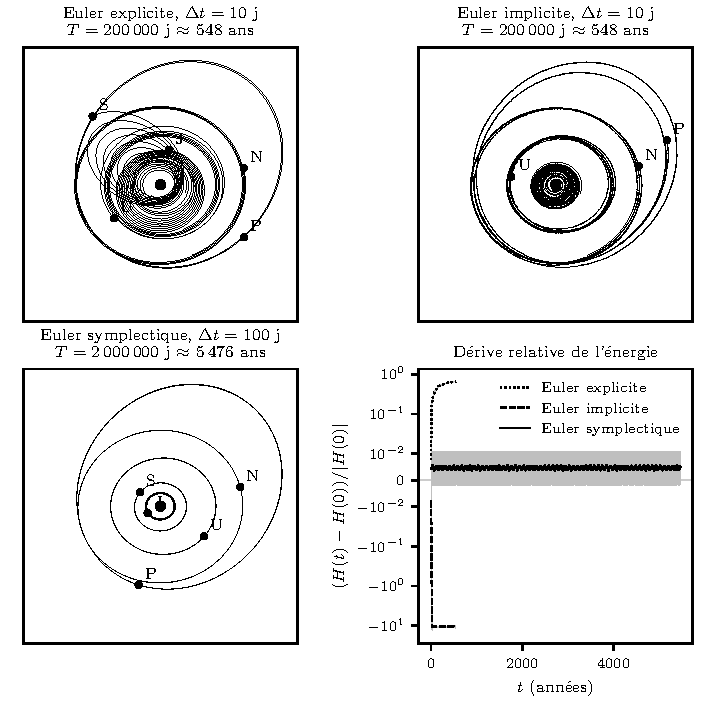
\includegraphics[width=\linewidth,height=0.55\textheight,keepaspectratio]{images/systeme_solaire.py.pdf}
\caption{Simulation du système solaire externe (Soleil, Jupiter, Saturne,
Uranus, Neptune, Pluton, données de (Hairer, Lubich, and Wanner
\protect\hyperlink{ed2-ref-Hairer10}{2010})) par les schémas d'Euler
explicite, implicite et symplectique, dans le référentiel du Soleil et
projetée dans le plan de l'écliptique. Avec Euler explicite, l'énergie augmente et les orbites de
Jupiter et Saturne s'ouvrent en spirale\,; avec Euler implicite, elle
diminue et les deux planètes tombent sur le Soleil en quelques
dizaines d'années. Le schéma symplectique, avec un pas dix fois plus
grand et un horizon dix fois plus long, conserve les orbites\,:
l'erreur sur l'énergie oscille à chaque révolution mais ne dérive pas.
En bas à droite, dérive relative de l'hamiltonien \(H\) (échelle
logarithmique de part et d'autre de \(\pm 10^{-2}\))\,: Euler explicite
gagne de l'énergie, Euler implicite en perd, massivement, jusqu'à la chute
de Jupiter\,; au-delà, le pas est bien trop grand pour résoudre l'orbite
numérique résiduelle et la simulation implicite n'a plus de sens.
%(en bas à droite, enveloppe de l'erreur relative sur l'hamiltonien\(H\)). 
%Le code générant cette figure est \texttt{images/systeme\_solaire.py}.
}\label{ed2-fig_systeme_solaire}
}
\end{figure}

\hypertarget{ed2-muxe9thodes-uxe0-un-pas}{%
\chapter{Méthodes à un pas}\label{ed2-muxe9thodes-uxe0-un-pas}}

\hypertarget{ed2-principe}{%
\section{Principe}\label{ed2-principe}}

Pour approximer les solutions d'une équation différentielle sur un
intervalle \([0,T]\), les méthodes numériques à un pas se basent sur la
représentation intégrale \[
x(t) = x_0 + \int_{t_0}^t f(s,x(s)) ds  = x_0 + \sum_{j=0}^{J-1} \int_{t_j}^{t_{j+1}}f(s,x(s)) ds
\] où \(t_0 < t_1 < \ldots < t_J\) avec \(t_J=T\). L'idée est
d'approximer les intégrales \(\int_{t_j}^{t_{j+1}}f(s,x(s))\) sur des
intervalles \([t_j,t_{j+1}]\) suffisamment petits.

Dans la suite, on note \(x^j\) l'approximation au temps \(t_j\) de la
valeur exacte \(x(t_j)\) et \({\Delta t}_j = t_{j+1}-t_j\) le \(j\)ème
pas de temps. L'idée est de calculer récursivement \[
x^{j+1} = x^j + {\Delta t}_j \Phi(t_j,x^j,{\Delta t}_j)
\] où \(\Phi(t_j,x^j,{\Delta t}_j)\) doit donc approximer \[
\frac{1}{t_{j+1}-t_j} \int_{t_j}^{t_{j+1}}f(s,x(s)) ds \ .
\] Les différentes méthodes de quadrature, i.e.~d'approximation de
l'intégrale, peuvent donc être mises à profit. La difficulté ici est que
seule la valeur initiale \(f(t_j,x(t_j))\) de \(f\) est connue (ou du
moins estimée) à l'itération \(j\), par \(f(t_j,x^j)\). On distingue
donc les méthodes \emph{explicites} où \(\Phi(t_j,x^j,{\Delta t}_j)\)
est écrite directement explicitement en fonction de la valeur initiale
\(x^j\), et les méthodes \emph{implicites} où cette expression n'est
connue qu'implicitement et des étapes intermédiaires de calcul sont
nécessaires.

\hypertarget{ed2-exemples}{%
\section{Exemples}\label{ed2-exemples}}

\begin{enumerate}
\def\labelenumi{\arabic{enumi}.}
\tightlist
\item
  Méthodes explicites:
\end{enumerate}

\begin{itemize}
\item
  Euler explicite: l'intégrale est approximée par l'aire d'un rectangle
  déterminé par la valeur initiale de \(f\) à \emph{gauche de
  l'intervalle}, i.e.\\
  \[
    x^{j+1} = x^j + {\Delta t}_j \, f(t_j,x^j) \ .
    \]
\item
  méthode de Heun~: l'intégrale est approximée par l'aire d'un trapèze
  déterminé par la valeur initiale de \(f\) et une approximation de sa
  valeur finale, i.e., \[
    x^{j+1} = x^j+\frac{{\Delta t}_j}{2}\Big(f(t_j,x^j) + f\big(t_{j+1},x^j+{\Delta t}_j f(t_j,x^j)\big) \Big) \ .
    \]
\item
  schéma de Runge--Kutta d'ordre 4: \[
  \left\{
  \begin{aligned}
  F_1 & = f(t_j,x^{j}) \\
  F_2 & = f\left(t_j+\frac{{\Delta t}_j}{2}, x^{j} + \frac{{\Delta t}_j}{2} F_1\right) \\
  F_3 & = f\left(t_j+\frac{{\Delta t}_j}{2}, x^{j} + \frac{{\Delta t}_j}{2} F_2\right) \\
  F_4 & = f(t_j + {\Delta t}_j, x^j + {\Delta t}_j F_3),
  \end{aligned}
  \right.
  \] et on pose \[
  x^{j+1} = x^{j} + {\Delta t}\, \frac{F_1 + 2F_2 + 2F_3 + F_4}{6} \ .
  \]
\end{itemize}

\begin{enumerate}
\def\labelenumi{\arabic{enumi}.}
\setcounter{enumi}{1}
\tightlist
\item
  Méthodes implicites:
\end{enumerate}

\begin{itemize}
\item
  Euler implicite~: l'intégrale est approximée par l'aire d'un rectangle
  déterminé par la valeur finale de \(f\) à \emph{droite de
  l'intervalle}, i.e.\\
  \[
    x^{j+1} = x^j + {\Delta t}_j \, f(t_{j+1},x^{j+1}) \ .
    \]
\item
  méthode des trapèzes (ou Crank--Nicolson)~: l'intégrale est approximée
  par l'aire du trapèze déterminé par les valeurs initiales et finales
  de \(f\), i.e.~ \[
  x^{j+1} = x^j+\frac{{\Delta t}_j}{2} \, \Big( f(t_j,x^j) + f(t_{j+1},x^{j+1})\Big) \ .
  \]
\item
  méthode du point milieu~: l'intégrale est approximée par l'aire d'un
  rectangle déterminé par une approximation de la valeur de \(f\) au
  milieu de l'intervale, i.e. \[
    x^{j+1} = x^j + {\Delta t}_j f\left(\frac{t_j+t_{j+1}}{2}, \frac{x^j+x^{j+1}}{2}\right) \ .
    \]
\end{itemize}

On peut bien sûr construire des méthodes plus compliquées et plus
précises pour des méthodes de Runge--Kutta d'ordre supérieur (explicites
ou implicites).

\hypertarget{ed2-sec_def_impl}{%
\section{\texorpdfstring{Définition implicite de
\(\Phi\)}{Définition implicite de \textbackslash Phi}}\label{ed2-sec_def_impl}}

Dans les schémas implicites, l'application \(\Phi\) est définie de
manière implicite. Par exemple, pour le schéma d'Euler, on a~: \[
\Phi(t_j,x^j,{\Delta t}_j) = f\Big(t_j + {\Delta t}_j, x^j + {\Delta t}_j\Phi(t_j,x^j,{\Delta t}_j) \Big).
\] Il faut donc s'assurer que \(\Phi\) est bien définie, c'est-à-dire
qu'il existe bien \(x^{j+1}\) tel que \[
x^{j+1} = x^j + {\Delta t}_j \, f(t_{j+1},x^{j+1}) \ .
\] Pour cela, nous pouvons voir \(x^{j+1}\) comme le point fixe de
l'application \(F_j\) définie par \[
F_j(x) = x^j + {\Delta t}_j \, f(t_{j+1},x) \ .
\] à \(x^j\), \({\Delta t}_j\), \(t_{j+1}\) fixés. L'existence (et
l'unicité) de ce point fixe peut alors être démontrée par le théorème de
point fixe de Banach. Si \(x\mapsto f(t_{j+1},x)\) est Lipschitzienne,
c'est-à-dire s'il existe \(L_j\) tel que \[
\|f(t_{j+1},x_a)-f(t_{j+1},x_b)\| \leq L_j \|x_a-x_b\| \qquad \forall (x_a,x_b)\in \mathbb{R}^n\times \mathbb{R}^n \ ,
\] alors \(F_j:\mathbb{R}^n \to \mathbb{R}^n\) est contractante pour un
pas de temps \({\Delta t}_j\) suffisamment petit puisque \[
\|F_j(x_a)-F_j(x_b)\| \leq  {\Delta t}_j L_j \|x_a-x_b\| \ .
\] Puisque \(\mathbb{R}^n\) est complet, on déduit par le théorème du
point fixe que \(x^{j+1}\) existe bien.

En pratique, on peut utiliser la méthode itérative de construction de ce
point fixe donnée par la preuve du théorème pour approcher \(x^{j+1}\).
Une stratégie est de partir de la valeur donnée par le schéma d'Euler
explicite \[
x^{j,0} = x^{j} + {\Delta t}_j f(t_j,x^{j})
\] et affiner ensuite par l'algorithme du point fixe en itérant \[
x^{j,k+1} = F(x^{j,k}) 
\] jusqu'à ce que l'évolution relative \[
\frac{x^{j,k+1}-x^{j,k}}{x^{j,0}}
\] devienne inférieure à un seuil choisi par l'utilisateur. Puisque la
suite \((x^{j,k})_{k\in \mathbb{N}}\) est de Cauchy, on sait que cette
algorithme s'arrête en un nombre fini d'itérations.

Notons que l'algorithme du point fixe n'est pas la seule façon de
résoudre l'équation \(x^{j+1} = F_j(x^{j+1})\)\,: c'est un système de
\(n\) équations non linéaires à \(n\) inconnues, \(G_j(x) = x - F_j(x) = 0\),
que l'on peut confier à n'importe quel solveur d'équations non linéaires,
typiquement la \emph{méthode de Newton} \[
x^{j,k+1} = x^{j,k} - \big(J_{G_j}(x^{j,k})\big)^{-1} G_j(x^{j,k}) \ ,
\] que l'on initialise là encore avec la prédiction du schéma explicite.
C'est ce que fait la fonction \texttt{scipy.optimize.fsolve} en Python,
et c'est la solution ``systématique''~: elle converge en quelques
itérations même lorsque \({\Delta t}_j L_j \geq 1\) et que \(F_j\) n'est
plus contractante, alors que l'algorithme du point fixe diverge. C'est
précisément dans ce régime, celui des pas de temps grands devant les
constantes de temps du système, que les schémas implicites sont
intéressants, et c'est pourquoi les solveurs implicites utilisent en
pratique une méthode de type Newton. Cette solution a ses limites~:

\begin{itemize}
\item
  chaque itération demande la jacobienne \(J_{G_j} = I - {\Delta t}_j J_f\)
  (calculée analytiquement, ou approchée par différences finies au prix de
  \(n\) évaluations supplémentaires de \(f\)) et la résolution d'un
  système linéaire de taille \(n\)\,: le coût par pas de temps croît vite
  avec la dimension\,;
\item
  Newton ne converge que depuis une initialisation suffisamment proche de
  la solution, et il n'y a aucune garantie si \({\Delta t}_j\) est
  trop grand~; le théorème de point fixe de Banach n'assure plus l'unicité
  de la solution, et le solveur peut converger vers une racine
  \emph{parasite} de \(G_j\), sans rien signaler. On l'observe
  par exemple sur le système raide de Robertson de la
  \protect\hyperlink{ed2-sec_systRaides}{section précédente (p.
  \pageref*{ed2-sec_systRaides})}, où un schéma d'Euler implicite résolu
  par \texttt{fsolve} converge pour \({\Delta t}=0{,}1\) vers une solution
  à concentrations négatives (voir le notebook Equations Differentielles II.ipynb)\,;
\item
  à l'inverse, si l'on choisit un pas de temps assez petit pour que
  \(F_j\) soit contractante, le point fixe est unique, l'algorithme de
  point fixe converge et n'exige aucune jacobienne~: c'est la méthode
  la plus simple, et elle suffit tant que l'on n'exploite pas la
  stabilité du schéma implicite pour prendre de grands pas.
\end{itemize}

Un tel schéma est plus lourd en terme de calculs qu'un algorithme
explicite mais il apporte en général plus de stabilité et permet souvent
d'utiliser un pas plus grand. C'est en particulier utile pour les
systèmes raides ou non-lisses, comme illustré dans l'exercice
\protect\hyperlink{ed2-exo_exp_impl}{\emph{Explicite ou Implicite?} (p.
\pageref*{ed2-exo_exp_impl})}.

\hypertarget{ed2-analyse-derreur}{%
\chapter{Analyse d'erreur}\label{ed2-analyse-derreur}}

L'objectif de l'analyse d'erreur \emph{a priori} est de donner une
estimation de l'erreur commise par la méthode numérique en fonction des
paramètres du problème (temps d'intégration, pas de temps, propriétés de
\(f\)). L'idée générale est de remarquer qu'à chaque pas de temps, on
commet une erreur d'intégration locale (erreur de troncature dans la
discrétisation de l'intégrale, à laquelle s'ajoutent souvent des erreurs
d'arrondi), et que ces erreurs locales s'accumulent au fil des pas. Le
contrôle de cette accumulation demande l'introduction d'une notion de
stabilité adéquate, alors que les erreurs locales sont liées à une
notion de consistance. L'alliance de stabilité et de consistante donne
une propriété de convergence qui est souhaitée lors de l'implémentation
de méthodes numériques.

\hypertarget{ed2-erreur-de-troncature-locale}{%
\section{Erreur de troncature
locale}\label{ed2-erreur-de-troncature-locale}}

L'erreur de troncature locale à l'itération \(j\) est l'erreur que l'on
commet en une seule itération lors de l'approximation de l'intégrale
pour passer de \(x^j\) à \(x^{j+1}\). C'est donc l'erreur théorique que
l'on obtiendrait si l'on appliquait le schéma numérique à la solution
exacte \(x(t_j)\). Elle est ainsi définie comme \[
\eta^{j+1} := \frac{x(t_{j+1}) - x(t_j) - {\Delta t}_j \Phi(t_j,x(t_j),{\Delta t}_j)}{{\Delta t}_j}.
\]

\hypertarget{ed2-def_consistance}{}
\addcontentsline{toc}{subsection}{Consistance}
\begin{definition}[Consistance]\label{ed2-def_consistance}
On note \({\Delta t}= \max_{0\le j\le J-1} {\Delta t}_j\) le pas de
temps maximal. On dit qu'une méthode numérique est \emph{consistante} si
\[
\lim_{{\Delta t}\to 0} \left( \max_{1\le j\le J} \|\eta^{j}\| \right) = 0 \ ,
\] et qu'elle est \emph{consistante d'ordre \(\geq p\)} s'il existe une
constante \(c_s\) telle que, pour tout \(0\le j\le J-1\), \[
\|\eta^{j+1}\| \le c_s \, ({\Delta t}_j)^{p} \ .
\] Une méthode est donc \emph{consistante d'ordre \(p\)} si elle est
consistante d'ordre \(\geq p\), mais pas \(\geq p+1\).
\end{definition}

\hypertarget{ed2-theo_CS_consistance}{}
\addcontentsline{toc}{subsection}{Condition nécessaire et suffisante de consistance}
\begin{theoreme}[Condition nécessaire et suffisante de consistance]\label{ed2-theo_CS_consistance}
Si \(\Phi\) est continue, alors le schéma est consistant si et seulement
si \[
\Phi(t,x,0) = f(t,x) \qquad \forall (t,x)\in \left[ 0,T \right]\times \mathbb{R}^n \ .
\]
\end{theoreme}

\hypertarget{ed2-duxe9monstration}{}
\begin{preuve}\label{ed2-duxe9monstration}
Soit \(C\) un ensemble fermé et borné tel que \(x(t)\in C\) pour tout
\(t\in \left[ 0,T \right]\). On note toujours
\({\Delta t}= \max_{0\le j\le J-1} {\Delta t}_j\). Par la représentation
intégrale des solutions, \[
x(t_{j+1}) = x(t_j) + \int_{t_j}^{t_{j+1}} f(x(s),s)ds
\] l'erreur de troncature locale s'écrit \[
\eta^{j+1} = \frac{1}{{\Delta t}_j}  \int_{t_j}^{t_{j+1}} \Big( f(s,x(s)) - \Phi(t_j,x(t_j),{\Delta t}_j) \Big)ds \ .
\] Si le schéma est consistant alors cette erreur tend vers 0 lorsque
\({\Delta t}\) tend vers 0 (pour n'importe quel système et n'importe
quelle trajectoire). Or, \[
\lim_{{\Delta t}\to 0} \frac{1}{{\Delta t}_j}  \int_{t_j}^{t_j+{\Delta t}} \Big( f(s,x(s)) - \Phi(t_j,x(t_j),{\Delta t}_j) \Big)ds = f(t_j,x(t_j)) - \Phi(t_j,x(t_j),0)
\] qui doit donc être nul.

Réciproquement, supposons \(\Phi(\cdot,\cdot,0)=f\). On doit montrer que
l'erreur de consistance tend vers 0 lorsque \({\Delta t}\) tend vers 0
(uniformément en \(j=1,\hdots,N\)). Soit \(\varepsilon >0\). Par la
continuité de \(\Phi\) et \(f\) et puisque \(\Phi(\cdot,\cdot,0)=f\), il
existe \(\Delta_1 >0\) tel que si \({\Delta t}\leq \Delta_1\), alors \[
\|\Phi(t,x,{\Delta t}_j) -f(t,x) \| \leq \varepsilon \qquad \forall (t,x) \in \left[ 0,T \right]\times C \quad \forall j=1,\hdots,N \ .
\] Donc \[
\|\eta^{j+1}\| \leq  \varepsilon + \frac{1}{{\Delta t}_j}  \int_{t_j}^{t_{j+1}} \big\| f(s,x(s)) - f(t_j,x(t_j)) \big\|ds \ .
\] Puisque \(s\mapsto f(s,x(s))\) est continue sur l'intervalle fermé et
borné \(\left[ 0,T \right]\), elle y est uniformément continue, donc il
existe \(\Delta_2 >0\) tel que si \({\Delta t}\leq \Delta_2\), \[
\big\| f(s,x(s)) - f(t_j,x(t_j)) \big\| \leq \varepsilon \qquad \forall s \in \left[ t_j,t_{j+1} \right]\quad \forall j=1,\hdots,N
\] et donc \(\|\eta^{j+1}\|\leq 2 \varepsilon\) pour tout \(j\). Le
schéma est donc bien consistant.\hfill$\blacksquare$
\end{preuve}

\hypertarget{ed2-ex_consistance}{}
\addcontentsline{toc}{subsubsection}{Schémas consistants}
\begin{exemple}[Schémas consistants]\label{ed2-ex_consistance}
Reprenons les exemples donnés plus haut.

\begin{itemize}
\item
  Euler explicite~: \(\Phi(t,x,{\Delta t})= f(t,x)\) indépendamment de
  \({\Delta t}\) donc la condition est trivialement satisfaite.
\item
  Méthode de Heun~:
  \(\Phi(t,x,{\Delta t}) = \frac{f(t,x) + f(t+{\Delta t},x+{\Delta t}f(t,x))}{2}\)
  donne bien \(f(t,x)\) si \({\Delta t}=0\).
\item
  Runge Kutta d'ordre 4~: lorsque \({\Delta t}=0\),
  \(F_1=F_2=F_3=F_4=f(t,x)\) donc
  \(\Phi(t,x,0) = \frac{F_1+2F_2+2F_3+F_4}{6}=f(t,x)\).
\end{itemize}

De même, la consistance des méthodes implicites s'obtiennent en
remarquant que \(x^{j+1}=x^{j}\) lorsque \({\Delta t}=0\).

Cette condition suffisante permet donc de prouver facilement le
caractère consistant d'un schéma. Cependant, en pratique, on s'intéresse
surtout à son ordre de consistance. Pour cela, l'erreur de consistance
se calcule souvent par des développements de Taylor des solutions
lorsque celles-ci sont suffisamment régulières, et la constante \(c_s\)
s'exprime alors comme une borne sur les dérivées des solutions. En fait,
on remarque que lorsque \(f\) est continue, la solution est \(C^1\) (par
définition de nos solutions). Mais puisque \(\dot{x}(t)=f(t,x(t))\),
\(\dot{x}\) hérite de la régularité de \(f\): si \(f\) est \(C^k\) alors
les solutions \(x\) sont \(C^{k+1}\). Le calcul de l'ordre de
consistance dans le cas dus schéma d'Euler explicite est donné
ci-dessous. Pour les autres schémas, voir l'exercice
\protect\hyperlink{ed2-exo_consist}{\emph{Consistance de schémas} (p.
\pageref*{ed2-exo_consist})}
\end{exemple}

\hypertarget{ed2-ex_consistance_Euler}{}
\addcontentsline{toc}{subsubsection}{Ordre de consistance du schéma d'Euler explicite}
\begin{exemple}[Ordre de consistance du schéma d'Euler explicite]\label{ed2-ex_consistance_Euler}
L'erreur de troncature s'écrit \[
\eta^{j+1} = \frac{x(t_j + {\Delta t}_j) - \Big( x(t_j) + {\Delta t}_j \, f(t_j,x(t_j)) \Big)}{{\Delta t}_j}.
\] Or, si \(f\) est \(C^1\), alors \(x\) est \(C^2\) et par application
la formule de Taylor avec reste intégral, on a \[
x(t_j + {\Delta t}_j) =  x(t_j) + {\Delta t}f(t_j,x(t_j))  + {\Delta t}_j^2 \int_{0}^{1} \ddot{x}(t_j+s{\Delta t}_j)  (1-s) ds ,
\] en utilisant \(\dot{x}(t_j)=f(t_j,x(t_j))\). Ceci donne donc \[
\|\eta^{j+1}\| \leq {\Delta t}_j  \int_{0}^{1} \ddot{x}(t_j+s{\Delta t}_j)  (1-s) ds \leq \frac{{\Delta t}_j}{2} \max_{t\in [t_j,t_{j+1}]} \|\ddot{x}(t)\| \leq \frac{{\Delta t}_j}{2} \max_{t\in [0,T]} \|\ddot{x}(t)\| \ .
\] Le schéma d'Euler explicite est donc consistant d'ordre \(\geq 1\)
avec \[
c_s= \frac{\max_{t\in [0,T]} \|\ddot{x}(t)\|}{2} \ .
\]

Notons qu'en utilisant \(\dot{x}(t) = f(t,x(t))\), \[
\ddot{x}(t) = \partial_t f(t,x(t)) + \partial_x f(t,x(t)) \cdot f(t,x(t)),
\] et on peut exprimer \(c_s\) en fonction de bornes sur \(x\) et sur
les dérivées de \(f\). Plus généralement, en dérivant successivement
lorsque \(f\) est \(C^k\), notons
\(f^{[k]} : \mathbb{R}\times \mathbb{R}^n \to \mathbb{R}^n\) la fonction
dépendant des dérivées successives de \(f\) telle que \[
x^{(k+1)}(t) = f^{[k]}(t,x(t)) \ .
\] On a alors le théorème suivant, généralisant les calculs précédents.
\end{exemple}

\hypertarget{ed2-theo_CS_consistance_ordre_p}{}
\addcontentsline{toc}{subsection}{\texorpdfstring{Condition nécessaire et suffisante de consistance d'ordre \(\geq p\)}{Condition nécessaire et suffisante de consistance d'ordre ≥ p}}
\begin{theoreme}[Condition nécessaire et suffisante de consistance d'ordre \(\geq p\)]\label{ed2-theo_CS_consistance_ordre_p}
Si \(\Phi\) et \(f\) sont \(C^p\) alors le schéma est consistant d'ordre
\(\geq p\) si et seulement si \[
\frac{\partial^k \Phi}{\partial {\Delta t}^k}(t,x,0) = \frac{1}{k+1}  f^{[k]}(t,x) \qquad \forall 0\leq k\leq p-1 \ , \quad \forall (t,x)\in \left[ 0,T \right]\times \mathbb{R}^n \ .
\]
\end{theoreme}

\hypertarget{ed2-duxe9monstration-1}{}
\begin{preuve}\label{ed2-duxe9monstration-1}
L'erreur de troncature s'écrit \[
\eta^{j+1} = \frac{x(t_j + {\Delta t}_j) - \Big( x(t_j) + {\Delta t}_j \, \Phi(t_j,x(t_j),{\Delta t}_j) \Big)}{{\Delta t}_j}.
\] Or, si \(f\) est \(C^p\), alors \(x\) est \(C^{p+1}\) et par
application la formule de Taylor avec reste intégral, on a
\begin{align*}
x(t_j + {\Delta t}_j) &= x(t_j) + \sum_{k=1}^p \frac{{\Delta t}_j^k}{k!}  x^{(k)} (t_j) +  \frac{{\Delta t}_j^{p+1}}{p!}\int_{0}^{1} x^{(p+1)}(t_j+s{\Delta t}_j)  (1-s)^p ds \\
&= x(t_j) + \sum_{k=0}^{p-1} \frac{{\Delta t}_j^{k+1}}{(k+1)!}  f^{[k]}(t_j,x(t_j)) +  \frac{{\Delta t}_j^{p+1}}{p!}\int_{0}^{1} x^{(p+1)}(t_j+s{\Delta t}_j)  (1-s)^p ds
\end{align*} Par ailleurs, puisque \(\Phi\) est \(C^p\), \[
\Phi(t,x,{\Delta t}) = \sum_{k=0}^{p-1} \frac{{\Delta t}^{k}}{k!}  \frac{\partial^k \Phi}{\partial {\Delta t}^k}(t,x,0) +  \frac{{\Delta t}^{p}}{(p-1)!}\int_{0}^{1} \frac{\partial^{p} \Phi}{\partial {\Delta t}^p}(t,x,t_j+s{\Delta t}_j)  (1-s)^{p-1} ds
\] Il s'ensuit que \[
\eta^{j+1} = \sum_{k=0}^{p-1} \frac{{\Delta t}_j^k}{k!} \left[ \frac{1}{k+1}  f^{[k]}(t_j,x(t_j)) - \frac{\partial^k \Phi}{\partial {\Delta t}^k}(t_j,x(t_j),0)\right] + {\Delta t}_j^p R_j
\] où \(R_j\) est borné (uniformément en \({\Delta t}_j\)) par
continuité de \(\frac{\partial^{p} \Phi}{\partial {\Delta t}^p}\) et
\(x^{(p+1)}\).

Maintenant, si le schéma est d'ordre \(\geq p\), alors
\(\frac{\eta^{j+1}}{{\Delta t}_j^p}\) doit rester borné lorsque
\({\Delta t}_j\) tend vers 0 et on obtient bien la condition du
théorème. Réciproquement, si la condition du théorème est vérifiée, on
obtient directement que \(\eta^{j+1}\) est borné en
\({\Delta t}_j^p\).\hfill$\blacksquare$
\end{preuve}

\hypertarget{ed2-ex_consistance_schemas}{}
\addcontentsline{toc}{subsubsection}{Ordre de consistance de schémas}
\begin{exemple}[Ordre de consistance de schémas]\label{ed2-ex_consistance_schemas}
On a vu que si \(f\) est \(C^1\), le schéma d'Euler explicite est
consistant d'ordre \(\geq 1\). On peut le retrouver ici en appliquant le
critère précédent pour \(p=1\) puisque \(\Phi(\cdot,\cdot,0)=f\).
Ensuite, si \(f\) est \(C^2\), on constate que \[
\frac{\partial\Phi}{\partial {\Delta t}}(t,x,0) = 0 \neq f^{[1]}(t,x) =\partial_t f(t,x) + \partial_x f(t,x) \cdot f(t,x)
\] donc le schéma d'Euler explicite est consistant d'ordre exactement
\(1\).

Par contre, toujours si \(f\) est \(C^2\), on constate que l'on a bien
pour le schéma de Heun \[
\frac{\partial\Phi}{\partial {\Delta t}}(t,x,0) =  f^{[1]}(t,x) =\partial_t f(t,x) + \partial_x f(t,x) \cdot f(t,x)
\] donc ce schéma est d'ordre \(\geq 2\). On peut vérifier que si \(f\)
est \(C^3\), le critère n'est pas vérifié à l'ordre supérieur donc il
est consistant d'ordre égal à 2.
\end{exemple}



\hypertarget{ed2-stabilituxe9}{%
\section{Stabilité}\label{ed2-stabilituxe9}}

Une fois que l'on a étudié l'erreur locale commise en une itération, on
s'intéresse à la manière dont elle va se propager au fur et à mesure des
itérations. Pour cela, la notion de stabilité quantifie la robustesse de
l'approximation numérique par rapport à l'accumulation des erreurs
locales et perturbations.

\hypertarget{ed2-def_stab}{}
\addcontentsline{toc}{subsection}{Stabilité}
\begin{definition}[Stabilité]\label{ed2-def_stab}
On dit qu'une méthode numérique est \emph{stable} s'il existe une
constante \(S(T) > 0\) (indépendente des \({\Delta t}_j\)) telle que,
pour toutes suites \(x = \{ x^j \}_{1 \leq j \leq J}\) et
\(z = \{ z^j \}_{1 \leq j \leq J}\) vérifiant \[
\left\{ \begin{aligned}
x^{j+1} & = x^j + {\Delta t}_j \Phi(t_j,x^j,{\Delta t}_j), \\
z^{j+1} & = z^j + {\Delta t}_j \Phi(t_j,z^j,{\Delta t}_j) + \delta^{j+1},
\end{aligned} \right.
\] on ait \[
\max_{1 \leq j \leq J} \| x^j - z^j\| \leq S(T) \, \Big( \|x^0 -z^0\| + \sum_{j = 1}^J  \|\delta^j\| \Big).
\]
\end{definition}

\hypertarget{ed2-theo_CS_stab}{}
\addcontentsline{toc}{subsection}{Condition suffisante de stabilité}
\begin{theoreme}[Condition suffisante de stabilité]\label{ed2-theo_CS_stab}
Si \(\Phi\) sont Lipschitziennes en \(x\), c'est-à-dire il existe
\(L>0\) tel que pour tout \(0\leq j\leq J\), \[
\|\Phi(t_j,x_a,{\Delta t}_j)-\Phi(t_j,x_b,{\Delta t}_j)\|\leq L \|x_a-x_b\| \qquad \forall (x_a,x_b)\in \mathbb{R}^n \times \mathbb{R}^n
\] alors le schéma est stable avec \(S(T)=e^{L T}\).
\end{theoreme}

\hypertarget{ed2-duxe9monstration-2}{}
\begin{preuve}\label{ed2-duxe9monstration-2}
On a alors \[
\| x^{j+1} - z^{j+1} \| \leq  \| \delta^{j+1} \| + (1 + {\Delta t}_j L) \| x^{j} - z^{j} \| \leq \| \delta^{j+1} \| +  e^{{\Delta t}_j L} \| x^{j} - z^{j} \| 
\] puisque \(1+x \leq e^{x}\) pour tout \(x\in \mathbb{R}\). Par
récurrence, on montre alors que pour tout \(1\leq j \leq J\), \[
\| x^{j} - z^{j} \| \leq e^{(t_j-t_0) L} \|x^0 -z^0\| + \sum_{k=1}^j e^{(t_j-t_k)L} \| \delta^{k} \|  \ .
\] Il s'ensuit que \[
\| x^{j} - z^{j} \| \leq e^{TL}\left(\|x^0 -z^0\|+ \sum_{k=1}^j \| \delta^{k} \|\right) \ ,
\] ce qui donne le résultat.\hfill$\blacksquare$
\end{preuve}

\hypertarget{ed2-convergence}{%
\section{Convergence}\label{ed2-convergence}}

La combinaison de consistance et de stabilité donne une propriété dite
de \emph{convergence} qui dit que l'erreur commise par le schéma par
rapport à la vraie solution converge vers 0 lorsque le pas de temps
converge vers 0. C'est une propriété cruciale pour un schéma numérique.

\hypertarget{ed2-def_conv}{}
\addcontentsline{toc}{subsection}{Convergence}
\begin{definition}[Convergence]\label{ed2-def_conv}
Soit \({\Delta t}= \max_{0 \leq j \leq J-1} {\Delta t}_j\). Un schéma
numérique est \emph{convergent} si \[
\lim_{{\Delta t}\to 0} \max_{1 \leq j \leq J} \|x^j - x(t_j)\| = 0
\] lorsque \(x^0 = x(t_0)\). S'il existe \(p\in \mathbb{N}_{>0}\) et
\(c_v>0\) (indépendent de \({\Delta t}\)) tel que \[
\max_{1 \leq j \leq J} \|x^j - x(t_j)\| \leq c_v ({\Delta t})^{p}
\] on dit que le schéma est \emph{convergent à l'ordre \(p\)}.
\end{definition}

\hypertarget{ed2-theo_Lax}{}
\addcontentsline{toc}{subsection}{Théorème de Lax}
\begin{theoreme}[Théorème de Lax]\label{ed2-theo_Lax}
Une méthode stable et consistante (à l'ordre \(p\)) est convergente (à
l'ordre \(p\)).
\end{theoreme}

\hypertarget{ed2-duxe9monstration-3}{}
\begin{preuve}\label{ed2-duxe9monstration-3}
Notons \(z^j=x(t_j)\). On remarque que \[
z^{j+1}  = z^j + {\Delta t}_j \Phi(t_j,z^j,{\Delta t}_j) + {\Delta t}_j\, \eta^{j+1},
\] où \(\eta\) est l'erreur de consistance. D'après la propriété de
stabilité, on a donc \[
\|x^j - x(t_j)\| \leq S(T) \,  \sum_{j = 1}^J {\Delta t}_{j-1}\, \|\eta^j\| \ ,
\] et par consistance \[
\|x^j - x(t_j)\| \leq S(T) \,  c_s \,  \sum_{j = 1}^J {\Delta t}_{j-1}\, ({\Delta t}_{j-1})^{p} \leq  c_s \, S(T) \, T \, ({\Delta t})^{p}  \ . 
\]\hfill$\blacksquare$
\end{preuve}

\hypertarget{ed2-theo_CS_conv}{}
\addcontentsline{toc}{subsection}{Condition suffisante de convergence}
\begin{theoreme}[Condition suffisante de convergence]\label{ed2-theo_CS_conv}
L'inconvénient du théorème de Lax est qu'il faut prouver la stabilité
pour obtenir la convergence. Or la seule condition suffisante dont nous
disposions à cet effet, est le caractère globalement Lipschitzien de
\(x\mapsto \Phi(t,x,{\Delta t})\). Mais il s'agit d'une condition très
forte. En fait, il est possible de prouver la convergence sous la
condition plus faible que \(x\mapsto \Phi(t,x,{\Delta t})\) est
``localement Lipschitzienne''~:

Si

\begin{enumerate}
\def\labelenumi{\arabic{enumi}.}
\item
  le schéma est consistant d'ordre \(p\),
\item
  pour tout boule fermée \(B\) de \(\mathbb{R}^n\), il existe \(L>0\),
  \({\Delta t}_m>0\) tels que pour tout \(t\in \left[ 0,T \right]\) et
  pour tout \({\Delta t}\in \left[ 0, {\Delta t}_m \right]\), \[
  \|\Phi(t_j,x_a,{\Delta t}_j)-\Phi(t_j,x_b,{\Delta t}_j)\|\leq L \|x_a-x_b\| \qquad \forall (x_a,x_b)\in B\times B 
  \]
\end{enumerate}

Alors il existe un pas de temps maximal \({\Delta t}_{\max}>0\) tel que
le schéma est convergent d'ordre \(p\).

L'hypothèse 2. est en particulier vérifiée si
\(x\mapsto \Phi(t,x,{\Delta t})\) est \(C^1\) d'après une version un peu
plus générale du théorème des accroissement finis.
\end{theoreme}

\hypertarget{ed2-ex_conv_Euler}{}
\addcontentsline{toc}{subsubsection}{Convergence du schéma d'Euler explicite}
\begin{exemple}[Convergence du schéma d'Euler explicite]\label{ed2-ex_conv_Euler}
On a déjà montré que le schéma d'Euler explicite est consistant d'ordre
1. Par ailleurs, si \(f\) est \(C^1\) par rapport à \(x\), alors
\(x\mapsto \Phi(t,x) = f(t,x,{\Delta t})\) est \(C^1\). Donc d'après le
théorème précédent, le schéma est convergent d'ordre 1.
\end{exemple}

Num\'eriquement, l'ordre de convergence des sch\'emas peut être visualis\'e en simulant une \'equation diff\'erentielle dont la solution analytique est connue, afin de tracer, en \'echelle log-log, l'erreur num\'erique de simulation en fonction du pas de temps\,: la pente de la courbe obtenue est l'ordre de convergence. C'est ce qui est fait sur la \protect\hyperlink{ed2-fig_ordre_schemas}{Figure~\ref*{ed2-fig_ordre_schemas} (p. \pageref*{ed2-fig_ordre_schemas})} pour les sch\'emas \`a un pas vus dans l'exercice \protect\hyperlink{ed2-exo_consist}{\emph{Consistance et ordre de sch\'emas} (p. \pageref*{ed2-exo_consist})}, sur le probl\`eme test \(\dot x = -x\), \(x(0)=1\), de solution \(x(t)=e^{-t}\). On retrouve les pentes \(1\), \(2\) et \(4\) d\'emontr\'ees analytiquement. Deux observations m\'eritent d'être soulign\'ees. D'une part, un sch\'ema implicite n'est pas plus pr\'ecis qu'un sch\'ema explicite\,: Euler implicite est d'ordre 1 comme Euler explicite, et ce que l'implicite apporte n'est pas de la pr\'ecision mais de la stabilit\'e (voir la \protect\hyperlink{ed2-sec_systRaides}{section sur les syst\`emes raides (p. \pageref*{ed2-sec_systRaides})}). D'autre part, pour le sch\'ema de Runge-Kutta 4, la courbe cesse de d\'ecro\^itre en dessous de \({\Delta t}\approx 10^{-3}\) et la pente ``casse''\,: l'erreur de troncature en \(({\Delta t})^4\) est alors devenue plus petite que la pr\'ecision de la machine, et ce sont les erreurs d'arrondi, accumul\'ees \`a chaque it\'eration, qui dominent. C'est l'objet de la section suivante.

\begin{figure}
\hypertarget{ed2-fig_ordre_schemas}{%
\centering
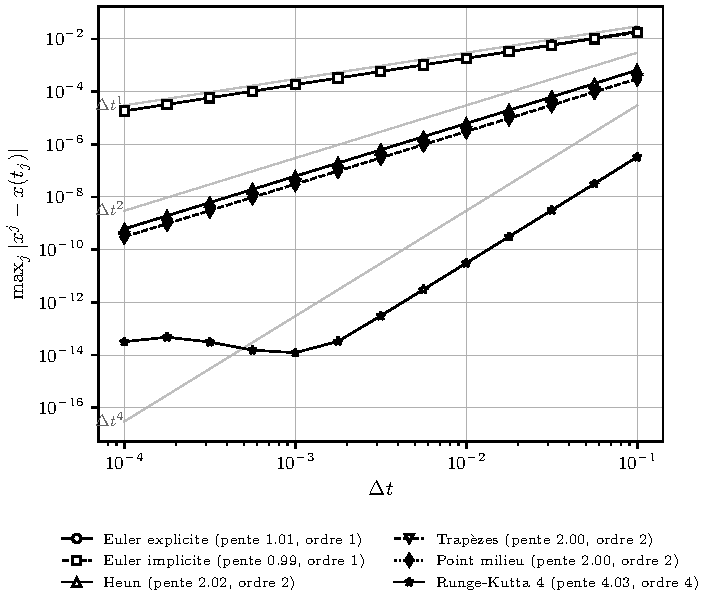
\includegraphics[width=\linewidth,height=0.5\textheight,keepaspectratio]{images/ordre_schemas.py.pdf}
\caption{Ordre de convergence exp\'erimental des sch\'emas \`a un pas du
cours sur le probl\`eme test \(\dot x = -x\), \(x(0)=1\), \(t\in[0,2]\)\,:
erreur globale \(\max_j |x^j-x(t_j)|\) en fonction du pas \({\Delta t}\)
(\'echelle log-log), et pente estim\'ee sur les six plus grands pas. Les
droites grises sont les r\'ef\'erences \(({\Delta t})^p\). 
%Le probl\`eme \'etant lin\'eaire, les sch\'emas des trap\`ezes et du point milieu co\"incident exactement. Pour Runge-Kutta 4, l'erreur sature autour de \(10^{-14}\) pour les petits pas\,: ce sont les erreurs d'arrondi. Le code g\'en\'erant cette figure est \texttt{images/ordre\_schemas.py}.
}\label{ed2-fig_ordre_schemas}
}
\end{figure}

\hypertarget{ed2-erreurs-darrondi-et-pas-optimal}{%
\section{Erreurs d'arrondi et pas
optimal}\label{ed2-erreurs-darrondi-et-pas-optimal}}

A chaque itération, lorsque la machine calcule \(x^{j+1}\), elle commet
en plus de l'erreur de troncature de l'intégrale des erreurs d'arrondi
de l'ordre de la précision machine. La solution obtenue est donc en fait
donnée par \[
\hat{x}^{j+1} = \hat{x}^j + {\Delta t}_j \left( \Phi(t_j,\hat{x}^j,{\Delta t}_j) + \rho^{j+1} \right)+ \varepsilon^{j+1}
\] au lieu de \[
x^{j+1} = x^j + {\Delta t}_j \Phi(t_j,x^j,{\Delta t}_j) \ ,
\] où \(\rho\) modélise l'erreur commise sur le calcul de \(\Phi\) et
\(\epsilon\) l'erreur sur l'addition finale. La stabilité nous donne
alors l'écart \[
\max_{0\leq j \leq J} \|x^j-\hat{x}^j\| \leq S(T) \sum_{j=1}^J {\Delta t}_{j-1} \|\rho^{j}\| + \|\varepsilon^{j}\| \ .
\] En considérant une borne \(\varepsilon\) des \(\varepsilon^{j}\) et
\(\rho\) des \(\rho^{j}\), on obtient \[
\max_{0\leq j \leq J} \|x^j-\hat{x}^j\| \leq S(T) (T\rho + J \varepsilon) \leq S(T) T \left(\rho + \frac{\varepsilon}{\min {\Delta t}_j} \right) \ ,
\] et donc finalement, en supposant l'algorithme convergent d'ordre
\(p\), \begin{align*}
\max_{0\leq j \leq J} \|x(t_j)-\hat{x}^j\| &\leq \max_{0\leq j \leq J} \|x(t_j)-x^j\| + \|x^j - \hat{x}^j\| \\
&\leq c_v (\max_j {\Delta t}_j)^p +  S(T) T \left(\rho + \frac{\varepsilon}{\min_j {\Delta t}_j} \right) \ .
\end{align*} Les paramètres \(\varepsilon\) et \(\rho\) sont typiquement
petits de l'ordre d'un facteur de la précision machine. Cependant, on
voit que plus le pas de temps décroit, plus il y a d'itérations et plus
les erreurs d'arrondi se propagent. D'un autre côté, plus il augmente,
plus les erreurs de quadrature augmentent. En supposant le pas constant,
il y a donc un pas ``optimal'\,' donné par \[
{\Delta t}_{opt} = \left( \frac{S(T) T\varepsilon}{c_vp}\right)^{\frac{1}{p+1}} \ .
\]

Ce ph\'enom\`ene est illustr\'e sur la \protect\hyperlink{ed2-fig_pas_optimal}{Figure~\ref*{ed2-fig_pas_optimal} (p. \pageref*{ed2-fig_pas_optimal})} avec le sch\'ema de Runge-Kutta 4 sur le probl\`eme test \(\dot x = -x\)\,: en diminuant le pas sur cinq ordres de grandeur, on voit l'erreur d\'ecro\^itre en \(({\Delta t})^4\), passer par un minimum autour de \(10^{-14}\), puis remonter. Plus l'ordre \(p\) est \'elev\'e, plus \({\Delta t}_{opt}\) est grand\,: un sch\'ema d'ordre \'elev\'e atteint la pr\'ecision machine avec un pas raisonnable, l\`a o\`u un sch\'ema d'ordre 1 demanderait un pas (et un nombre d'it\'erations) d\'eraisonnable. Il est donc illusoire de chercher \`a am\'eliorer la pr\'ecision en diminuant ind\'efiniment le pas\,: en pratique, on travaille toujours avec \({\Delta t}\gg {\Delta t}_{opt}\), et c'est le choix du sch\'ema et l'adaptation du pas (voir l'\protect\hyperlink{ed2-annexe-choix-du-pas-de-temps}{annexe (p. \pageref*{ed2-annexe-choix-du-pas-de-temps})}) qui permettent de contr\^oler l'erreur.

\begin{figure}
\hypertarget{ed2-fig_pas_optimal}{%
\centering
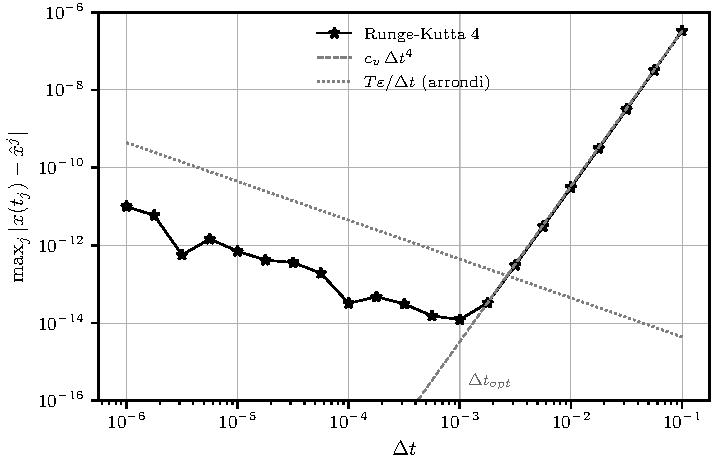
\includegraphics{images/pas_optimal.py.pdf}
\caption{Erreur globale du sch\'ema de Runge-Kutta 4 sur \(\dot x = -x\),
\(x(0)=1\), \(t\in[0,2]\) en fonction du pas, en double pr\'ecision
(\(\varepsilon\approx 2\cdot 10^{-16}\)). Pour les grands pas, l'erreur de
troncature \(c_v({\Delta t})^4\) domine\,; pour les petits pas, les erreurs
d'arrondi accumul\'ees sur les \(T/{\Delta t}\) it\'erations dominent et
l'erreur remonte lorsque le pas diminue. La borne \(T\varepsilon/{\Delta t}\)
du cours est un pire cas\,: en pratique les erreurs d'arrondi se compensent
partiellement et la remont\'ee observ\'ee est en dessous de cette borne. 
%Le pas optimal est au voisinage de la rencontre des deux asymptotes. Le code g\'en\'erant cette figure est \texttt{images/pas\_optimal.py}.
}\label{ed2-fig_pas_optimal}
}
\end{figure}

\hypertarget{ed2-annexe-choix-du-pas-de-temps}{%
\chapter{Annexe -- Choix du pas de
temps}\label{ed2-annexe-choix-du-pas-de-temps}}

Jusqu'à présent, on a présenté des schémas dépendant de pas de temps
\({\Delta t}_j\), sans jamais dire comment les choisir. Le plus simple
est de choisir un pas \({\Delta t}\) fixe mais il est difficile de
savoir à l'avance quel pas est nécessaire. En particulier, comment
savoir si la solution obtenue est suffisamment précise, sans connaître
la vraie\,?

\hypertarget{ed2-pas-fixe}{%
\section{Pas fixe}\label{ed2-pas-fixe}}

Une voie empirique est de fixer un pas, lancer la simulation, puis fixer
un pas plus petit, relancer la simulation, jusqu'à ce que les résultats
\emph{ne semble plus changer} (au sens de ce qui nous intéresse
d'observer). Notons que la connaissance des constantes de temps
présentes dans le système peut aider à fixer un premier ordre de
grandeur du pas. On pourrait aussi directement choisir le pas
\({\Delta t}_{opt}\) obtenu plus haut en prenant en compte les erreurs
d'arrondis. Mais les constantes \(c_v\) et \(S(T)\) sont souvent mal
connues et conservatives.

\hypertarget{ed2-adaptation-du-pas-de-temps}{%
\section{Adaptation du pas de
temps}\label{ed2-adaptation-du-pas-de-temps}}

Les méthodes à pas fixe exploitent la convergence des schémas, mais

\begin{itemize}
\item
  on ne peut pas prendre un pas de temps arbitrairement petit car on est
  contraint par le temps de simulation.
\item
  on n'a aucune idée de l'erreur commise et on n'est jamais sûr d'avoir
  la bonne solution.
\item
  l'utilisation d'un pas très petit peut n'être nécessaire qu'autour de
  certains points \emph{sensibles} (proches de singularités par exemple)
  et consomme des ressources inutiles ailleurs.
\end{itemize}

L'idée serait donc plutôt d'adapter la valeur du pas \({\Delta t}_j\) à
chaque itération. En d'autres termes, on se fixe une tolérance d'erreur
que l'on juge acceptable et on modifie le pas de temps en ligne, selon
si l'on estime être au-dessus ou en-dessous du seuil d'erreur. Mais cela
suppose d'avoir une idée de l'erreur commise\ldots{} Il existe justement
des moyens de l'estimer.

Tout d'abord, de quelle erreur parle-t-on\,?

\begin{itemize}
\item
  erreur \emph{globale}\,? L'idéal serait de contrôler
  \(\max_{0\leq j\leq N} \|x^j - x(t_j)\|\). Or la stabilité nous dit
  que \[
  \max_{0\leq j\leq N} \|x^j - x(t_j)\| \leq S(T) \,  \sum_{j = 1}^J {\Delta t}_{j-1}\, \|\eta^j\|
  \] avec \(\eta^j\) les erreurs de consistances locales. Donc si on se
  fixe une tolérance sur l'erreur globale \(\texttt{Tol}_g\), on a \[
  \|\eta^j\| \leq \frac{\texttt{Tol}_g}{TS(T)} \qquad \Longrightarrow \qquad \max_{0\leq j\leq N} \|x^j - x(t_j)\| \leq \texttt{Tol}_g \ .
  \] En d'autre termes, \(\texttt{Tol}_g\) nous fixe une erreur maximale
  \emph{locale} sur \(\eta^j\), à chaque itération. Notons cependant que
  cette borne ne prend pas en compte la propagation des erreurs
  d'arrondis~: plus \({\Delta t}\) diminue, plus l'erreur globale risque
  d'augmenter. Ce phénomène devrait donc en toute rigueur aussi nous
  donner un pas de temps minimal \({\Delta t}_{\min}\). Notons que tous
  ces calculs dépendent des constantes \(c_v\) et \(S(T)\) qui sont
  souvent mal connues ou très conservatives.
\item
  erreur (absolue) \emph{locale}\,? A chaque itération, une erreur
  locale est commise dûe à l'approximation de l'intégrale. Cette erreur
  est donnée par \[
  e^{j+1} = \tilde{x}(t_{j+1}) -x^{j+1} = \left(x^j + \int_{t_j}^{t_{j+1}} f(s,\tilde{x}(s))ds\right)
  \] où \(\tilde{x}\) est la solution de \(\dot{x}=f(t,x)\) qui serait
  initialisée à \(x^j\) au temps \(t_j\). Notons que si on avait
  \(x^j=x(t_j)\), on aurait exactement
  \(e^{j+1}={\Delta t}_j \eta^{j+1}\), où \(\eta^{j+1}\) est l'erreur de
  consistance. On se donne donc une tolérance d'erreur locale \[
  \|e^{j+1}\| \leq \texttt{Tol}_{abs} \ .
  \]
\item
  erreur \emph{relative}\,? Fixer une erreur absolue est parfois trop
  contraignant et n'a de sens que si les solutions gardent un certain
  ordre de grandeur. En effet, l'erreur acceptable quand la solution
  vaut 1000 n'est peut-être pas la même que lorsqu'elle vaut 1. On peut
  donc plutôt exiger une certaine erreur relative
  \(\texttt{Tol}_{rel}\), i.e., \[
  \frac{\|e^{j+1}\|}{\|x^j\|}\leq \texttt{Tol}_{rel} \ .
  \]
\end{itemize}

En général, les solvers assurent (approxivement) \[
\|e^{j+1}\| \leq \texttt{Tol}_{abs} + \texttt{Tol}_{rel} \|x^j\| \ .
\] Par défaut, dans les solvers de Numpy,
\(\texttt{Tol}_{abs} = 10^{-6}\) et \(\texttt{Tol}_{rel}= 10^{-3}\).

Mais pour cela nous devons trouver un moyen d'estimer l'erreur locale.
C'est souvent fait en utilisant une même méthode à deux pas différents
(par exemple \({\Delta t}_j\) et \({\Delta t}_j/2\)), ou bien en
imbriquant des schémas de Runge-Kutta d'ordres différents.

En fait, il est possible de montrer (exercice) que si \(f\) est \(C^1\),
on a pour un schéma d'Euler explicite \[
\|e^{j+1}\| = {\Delta t}_j \, \frac{\big\|f(t_{j+1},x^{j+1}) - f(t_j,x^j)\big\|}{2} + o({\Delta t}_j^2) \ 
\]

On peut donc estimer à chaque itération l'erreur commise \(e^{j+1}\) et
adapter le pas selon si celle-ci est inférieure ou supérieure au seuil
de tolérance. En effet, puisque l'on sait par ailleurs que
\(e^{j+1} = O({\Delta t}_j^2)\), une possible stratégie d'adaptation est
de prendre\\
\[
{\Delta t}_{new} = {\Delta t}_j \sqrt{\frac{\texttt{Tol}_{abs}}{\|e^{j+1}\|}}
\] (éventuellement avec une marge de sécurité)

La fonction correspondante
\begin{verbatim}
def solve_euler_explicit_variable_step(f, x0, t0, tf, dtmin, dtmax, atol):
  ...
  return t, x
\end{verbatim}
est fournie dans le notebook Equations Differentielles II.ipynb.
La \protect\hyperlink{ed2-fig_van_der_pol}{Figure~\ref*{ed2-fig_van_der_pol}
(p. \pageref*{ed2-fig_van_der_pol})} montre cette stratégie à l'\oe uvre
sur l'oscillateur de Van der Pol \[
\dot{y}_1 = y_2 \quad , \qquad \dot{y}_2 = \mu (1-y_1^2)\, y_2 - y_1
\] avec \(\mu = 10\) et \(y(0) = (2,0)\). Pour \(\mu\) grand, ce système
présente des \emph{oscillations de relaxation}\,: la solution alterne
entre des phases lentes, où elle suit de près une courbe en S dans le
plan de phase, et des sauts rapides quasi verticaux d'une branche de
cette courbe à l'autre. Le système est autonome\,: ce n'est pas le temps
qui rend \(f\) grande, c'est la trajectoire elle-même qui revient
périodiquement dans les régions de l'espace d'état (au voisinage de
\(y_1=\pm 1\)) où \(f\) et sa dérivée \(f^{[1]}\), donc l'erreur de
consistance, explosent. Le pas se resserre d'un facteur mille pendant
chaque saut puis se relâche jusqu'à \({\Delta t}_{\max}\) sur les
phases lentes, indéfiniment et en phase avec le cycle limite. Un pas
fixe devrait être choisi à la plus petite de ces valeurs partout. Notons
enfin que cette stratégie ne contrôle que l'erreur \emph{locale}\,: rien
ne garantit l'erreur globale, qui dépend de la constante de stabilité
\(S(T)\)\,; et que pour \(\mu\) plus grand encore, le système devient
franchement raide (voir la
\protect\hyperlink{ed2-sec_systRaides}{section sur les systèmes raides
(p. \pageref*{ed2-sec_systRaides})}) et le pas d'un schéma explicite
s'effondrerait pendant les sauts\,: il faudrait alors passer à un schéma
implicite.

\begin{figure}
\hypertarget{ed2-fig_van_der_pol}{%
\centering
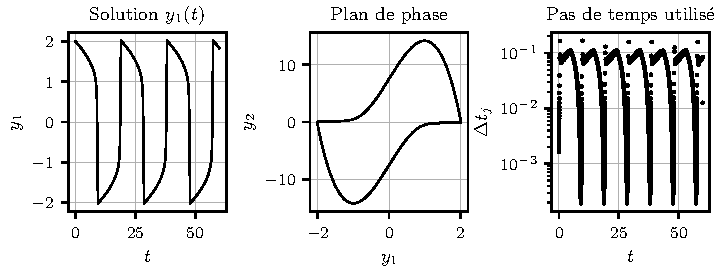
\includegraphics[width=\linewidth]{images/van_der_pol_pas_adaptatif.py.pdf}
\caption{Euler explicite à pas adaptatif sur l'oscillateur de Van der
Pol (\(\mu=10\), \(y(0)=(2,0)\), \(\texttt{Tol}_{abs}=10^{-4}\),
\({\Delta t}\in[10^{-6},0{,}2]\)). De gauche à droite\,: la solution
\(y_1(t)\), le plan de phase, et le pas \({\Delta t}_j\) retenu à chaque
itération (échelle logarithmique), qui se resserre à chaque saut du
cycle limite. 
%Le code générant cette figure est \texttt{images/van\_der\_pol\_pas\_adaptatif.py}.
}\label{ed2-fig_van_der_pol}
}
\end{figure}

\hypertarget{ed2-exercices}{%
\chapter{Exercices}\label{ed2-exercices}}

\hypertarget{ed2-exo_consist}{%
\section{Consistance et ordre de schémas}\label{ed2-exo_consist}}

Supposons \(f\) de classe \(C^2\). Montrer que~:

\hypertarget{ed2-consist-1}{%
\subsubsection*{Question 1}\label{ed2-consist-1}}

\addcontentsline{toc}{subsubsection}{Question 1}

le schéma de Heun est consistant d'ordre \(\geq 2\) et égal à 2 si \(f\)
est \(C^3\).\solref{ed2-answer-consist-1}

\hypertarget{ed2-consist-2}{%
\subsubsection*{Question 2}\label{ed2-consist-2}}

\addcontentsline{toc}{subsubsection}{Question 2}

le schéma d'Euler implicite est consistant d'ordre \(\geq 1\)\solref{ed2-answer-consist-2}

\hypertarget{ed2-consist-3}{%
\subsubsection*{Question 3}\label{ed2-consist-3}}

\addcontentsline{toc}{subsubsection}{Question 3}

la méthode des trapèzes est consistante d'ordre \(\geq 2\).\solref{ed2-answer-consist-3}

\hypertarget{ed2-consist-4}{%
\subsubsection*{Question 4}\label{ed2-consist-4}}

\addcontentsline{toc}{subsubsection}{Question 4}

le schéma du point milieu est consistant d'ordre \(\geq 2\).\solref{ed2-answer-consist-4}

\hypertarget{ed2-consist-5}{%
\subsubsection*{Question 5}\label{ed2-consist-5}}

\addcontentsline{toc}{subsubsection}{Question 5}

le schéma de Runge-Kutta d'ordre 4 est bien consistant d'ordre \(4\) si
\(f\) est \(C^5\).\solref{ed2-answer-consist-5}

On supposera le pas suffisamment petit pour que les schémas implicites
soient définis.

\hypertarget{ed2-conv}{%
\section{Convergence de schémas}\label{ed2-conv}}

Sous l'hypothèse que \(f\) est \(C^1\), montrer que les schémas de Heun
et d'Euler implicite sont convergents.\solref{ed2-answer-conv}

\hypertarget{ed2-exo_exp_impl}{%
\section{Explicite ou implicite\,?}\label{ed2-exo_exp_impl}}

Commençons par consid\'erer le cas des syst\`emes raides.

\hypertarget{ed2-impl-1}{%
\subsubsection*{Question 1}\label{ed2-impl-1}}

\addcontentsline{toc}{subsubsection}{Question 1}

Comparer les performances des schémas d'Euler implicites et explicites à
pas fixe dans le cas de \(\dot{x} = -\lambda x\), \(x(0)=1\), et
\(\dot{x} = \lambda x\), \(x(0)=1\), sur un horizon de temps \(T\)
donné.\solref{ed2-answer-impl-1}

\hypertarget{ed2-impl-2}{%
\subsubsection*{Question 2}\label{ed2-impl-2}}

\addcontentsline{toc}{subsubsection}{Question 2}

Lorsqu'on modélise des systèmes chimiques ou biologiques, on obtient
souvent des réactions aux constantes de temps très différentes. Vaut-il
mieux utiliser un schéma d'Euler implicite ou explicite pour simuler \[
\dot{x} = \left(
  \begin{matrix}
  -1 & 0 \\
  0 & -\mu
  \end{matrix}
  \right) x 
\] avec \(\mu >> 1\)\,?\solref{ed2-answer-impl-2}

\vspace{1em}
Consid\'erons maintenant le cas des syst\`emes non-lisses. Un solide freiné par un frottement sec (de Coulomb) subit une force de
module constant, toujours opposée à sa vitesse. En notant \(x\) la
vitesse, le modèle le plus simple est \[
\dot{x} = -\mathrm{sign}(x) \qquad , \qquad x(0) = x_0 \ ,
\] avec la convention \(\mathrm{sign}(0) = 0\). La fonction
\(\mathrm{sign}\) n'étant pas continue en 0, les théorèmes du chapitre
I ne s'appliquent pas tels quels\,: on cherche ici une solution
continue, dérivable sauf en un nombre fini d'instants, qui vérifie
l'équation partout ailleurs.

\hypertarget{ed2-impl-3}{%
\subsubsection*{Question 3}\label{ed2-impl-3}}

\addcontentsline{toc}{subsubsection}{Question 3 (Frottement sec)}

\begin{enumerate}
\def\labelenumi{\alph{enumi})}
\tightlist
\item
  Déterminer la solution pour \(x_0>0\), puis pour \(x_0\) quelconque.
  Qu'a-t-elle de remarquable par rapport à celle de
  \(\dot{x}=-\lambda x\)\,? Un tel comportement serait-il possible pour
  une équation \(\dot{x}=f(x)\) avec \(f\) continûment différentiable\,?
\item
  Ecrire le schéma d'Euler explicite de pas \({\Delta t}\) et décrire
  précisément le comportement de la suite \((x^j)\) à partir de
  \(x_0>0\), en particulier lorsqu'elle arrive au voisinage de 0.
  Diminuer le pas résout-il le problème\,?
\item
  Ecrire le schéma d'Euler implicite et montrer que, pour
  \(0<|x^j|\leq {\Delta t}\), l'équation définissant \(x^{j+1}\) n'a pas
  de solution avec la convention \(\mathrm{sign}(0)=0\). Montrer qu'en
  autorisant \(\mathrm{sign}(0)\) à prendre n'importe quelle valeur dans
  \([-1,1]\) (c'est la régularisation naturelle de la discontinuité),
  l'équation admet au contraire une unique solution pour tout \(x^j\),
  que l'on explicitera.
\item
  En déduire la suite \((x^j)\) produite par le schéma implicite et
  justifier qu'il résout le problème observé en b). 
  %Quelle propriété de
  %l'application \(x \mapsto x + {\Delta t}\,\mathrm{sign}(x)\), absente
  %de \(x \mapsto x - {\Delta t}\,\mathrm{sign}(x)\), est responsable de
  %cette différence\,?
\end{enumerate}\solref{ed2-answer-impl-3}

\hypertarget{ed2-exo_symplectique}{%
\section{Euler symplectique}\label{ed2-exo_symplectique}}

Pour \(\omega>0\) donné, considérons le système \[
\dot{x}_1 \;=\;  x_2
\quad ,\qquad 
\dot{x}_2(t)\;=\; -\omega^2 x_1
\] de condition initiale \(x(0)\;=\; (1,0)\). On rappelle que pour une
suite de la forme \(x^{j+1}=A x^j\) converge vers 0 si les valeurs
propres de \(A\) sont à l'intérieur du cercle unité et diverge si au
moins une valeur propre est à l'extérieur.

\hypertarget{ed2-symp-1}{%
\subsubsection*{Question 1}\label{ed2-symp-1}}

\addcontentsline{toc}{subsubsection}{Question 1}

Montrer que pour n'importe quel pas \({\Delta t}\) fixé, un schéma
d'Euler explicite donne une solution divergente, et un schéma d'Euler
implicite donne une solution qui converge vers 0. Lequel a raison\,?\solref{ed2-answer-symp-1}

On définit maintenant le schéma suivant qui ``mélange'\,' les schémas
d'Euler implicites et explicites~: \begin{align*}
x^{j+1}_1 &= x^{j}_1 + {\Delta t}\, x^{j}_2 \\
x^{j+1}_2 &= x^{j}_2 - {\Delta t}\, \omega^2 x^{j+1}_1
\end{align*}

\hypertarget{ed2-symp-2}{%
\subsubsection*{Question 2}\label{ed2-symp-2}}

\addcontentsline{toc}{subsubsection}{Question 2}

Montrer que la quantité
\(\omega^2 x_1^2 + x_2^2 +{\Delta t}\, \omega^2 x_1x_2\) est conservée.
Quelle est alors la forme des solutions obtenues dans le plan de phase
si \(\omega {\Delta t}<2\)\,? En déduire la pertinence de ce schéma. On
parle de schéma \emph{symplectique}, car il conserve les volumes.\solref{ed2-answer-symp-2}

\hypertarget{ed2-symp-3}{%
\subsubsection*{Question 3}\label{ed2-symp-3}}

\addcontentsline{toc}{subsubsection}{Question 3}

En écrivant le schéma sous la forme \(x^{j+1}=Ax^j\), montrer qu'il
diverge par contre si \({\Delta t}\, \omega > 2\).\solref{ed2-answer-symp-3}

\hypertarget{ed2-symp-4}{%
\subsubsection*{Question 4}\label{ed2-symp-4}}

\addcontentsline{toc}{subsubsection}{Question 4}

Plus généralement, proposer un schéma pour simuler un système
Hamiltonien du type \begin{align*}
\dot{q} &= \nabla_p H(q,p) \\
\dot{p} &= - \nabla_q H(q,p)
\end{align*} où \((q,p)\in \mathbb{R}^N \times \mathbb{R}^N\) sont les
positions généralisées et quantités de mouvement, \(H\) est le
Hamiltonien que l'on pourra vérifier être conservé le long des
trajectoires.\solref{ed2-answer-symp-4}

A noter que les conclusions de cet exercice sont les mêmes si l'on
utilise un schéma d'Euler implicite sur la première composante et un
schéma d'Euler explicite sur la deuxième. Ces deux schémas s'appellent
respectivement Euler symplectique A et B.

\hypertarget{ed2-ruxe9fuxe9rences}{%
\chapter{Références}\label{ed2-ruxe9fuxe9rences}}

\hypertarget{ed2-refs}{}
\begin{cslreferences}
\leavevmode\hypertarget{ed2-ref-Dem06}{}%
Demailly, J.-P. 2006. \emph{Analyse Numérique et équations
Différentielles}. EDP Sciences. Grenoble Sciences.

\leavevmode\hypertarget{ed2-ref-Hairer10}{}%
Hairer, E., C. Lubich, and G. Wanner. 2010. \emph{Geometric Numerical
Integration : Structure-Preserving Algorithms for Ordinary Differential
Equations}. Edited by Springer Series in Computational Mathematics. 2nd
ed. Springer-Verlag, Berlin.

\leavevmode\hypertarget{ed2-ref-Hairer96}{}%
Hairer, E., and G. Wanner. 1996. \emph{Solving Ordinary Differential
Equations II. Stiff and Differential-Algebraic Problems}. Edited by
Springer Series in Computational Mathematics. 2nd ed. Springer-Verlag,
Berlin.
\end{cslreferences}


%% Corrections regroupées en fin de poly. Pour imprimer sans les corrections : \correctionsfalse
%% dans le préambule ; les renvois "(Solution p. x.)" des énoncés disparaissent alors aussi.
\ifcorrections
\part{Corrections des exercices}
\hypertarget{solutions-des-exercices}{%
\chapter{Etude théorique des solutions}\label{solutions-des-exercices}}

\hypertarget{exercices-essentiels}{%
\section{Exercices essentiels}\label{exercices-essentiels}}

\hypertarget{answer-glob_sol}{%
\subsubsection*{Solutions globales I}\label{answer-glob_sol}}

\addcontentsline{toc}{subsubsection}{Solutions globales I}

Fixons une condition initiale dans \(\mathbb{R}\times \mathbb{R}^2\). La
fonction
\(f:(t,x_1,x_2)\mapsto (\sin x_1 - \sqrt{|t|} x_2 ,\sqrt{1+x_1^2})\) est
continue sur \(\mathbb{R}\times\mathbb{R}^2\). Donc d'après le théorème
de Peano des solutions existent. D'après le théorème du domaine maximal
d'existence, les solutions maximales sont définies sur un intervalle de
temps \(I\) ouvert.

Par ailleurs, on peut vérifier que pour tout \(y\in \mathbb{R}\),
\(\sqrt{1+y^2}\leq 1+|y|\), donc \[
|f_1(x)| \leq 1 + \sqrt{|t|} |x_2| \quad , \quad |f_2(x)|\leq 1 + |x_1|
\] et \(f\) est bornée par une fonction affine en \(\|x\|\). Toutes les
solutions maximales sont donc globales, i.e.~\(I=\mathbb{R}\).

\hypertarget{answer-glob_sol2}{%
\subsubsection*{Solutions globales II}\label{answer-glob_sol2}}

\addcontentsline{toc}{subsubsection}{Solutions globales II}

Considérons une condition initiale dans
\(\mathbb{R}\times \mathbb{R}^n\) et une solution maximale
\(t\mapsto x(t)\) définie sur un intervalle \(I\) (qui existe d'après le
théorème de Peano car \(f\) est continue sur
\(\mathbb{R}\times \mathbb{R}^n\)). Alors \[
\frac{d}{dt} V(x(t)) = \langle\nabla V (x(t)), f(t,x(t))\rangle \leq a(t) V(x(t)) + b(t) \quad \forall t\in I \ ,
\] et donc \[
\frac{d}{dt} \left[e^{-\int_{t_0}^t a(\tau) d\tau}  V(x(t))\right] \leq e^{-\int_{t_0}^t a(\tau) d\tau} b(t)  \quad \forall t\in I \ .
\] En intégrant entre \(t_0\) et \(t\geq t_0\), \[
e^{-\int_{t_0}^t a(\tau) d\tau} V(x(t)) - V(x(t_0)) \leq \int_{t_0}^t e^{-\int_{t_0}^s a(\tau) d\tau} b(s) ds \quad \forall t\in I \cap [t_0,+\infty[
\] et donc \[
V(x(t)) \leq e^{\int_{t_0}^t a(\tau) d\tau} V(x(t_0)) + \int_{t_0}^t e^{\int_{s}^t a(\tau) d\tau} b(s) ds \quad \forall t\in I \cap [t_0,+\infty[ \ .
\] Une autre manière de faire est de montrer que \(V(x(t))\leq v(t)\) où
\(v\) est solution maximale de \[
\dot{v} = a(t) v + b(t)
\] pour la condition initiale \(v(t_0) = V(x(t_0))\), qui est définie
et continue sur \(\mathbb{R}\) car la dynamique de \(v\) est affine.

Or si \(\tmax= \sup I\) est fini, d'après le théorème du domaine
maximal, \((t,x(t))\) tend soit vers la frontière du domaine de
définition de \(f\), soit diverge. Comme \(f\) est définie et continue
sur \(\mathbb{R}\times \mathbb{R}^n\), nécessairement
\(\lim_{t\to \tmax} \|x(t)\| = +\infty\) et donc
\(\lim_{t\to \tmax} V(x(t)) = +\infty\). Or par continuité de \(a,b\)
sur \(\mathbb{R}\), \[
\lim_{t\to \tmax} V(x(t)) \leq e^{\int_{t_0}^{\tmax} a(\tau) d\tau} V(x(t_0)) + \int_{t_0}^{\tmax} e^{\int_{s}^{\tmax} a(\tau) d\tau} b(s) ds   \ .
\] C'est donc impossible et \(\tmax= +\infty\).

\hypertarget{answer-glob_sol3}{%
\subsubsection*{Solutions globales III}\label{answer-glob_sol3}}

\addcontentsline{toc}{subsubsection}{Solutions globales III}

Considérons une condition initiale dans
\(\mathbb{R}\times \mathbb{R}^n\) et une solution maximale
\(t\mapsto x(t)\) définie sur un intervalle \(I\). Alors \[
\frac{d}{dt} V(x(t)) = \langle\nabla V (x(t)), f(t,x(t))\rangle \leq 0 \quad \forall t\in I \ ,
\] donc \(t\mapsto V(x(t))\) décroît et est donc bornée en temps positif
par \(V(x(t_0))\). D'après le théorème du domaine maximal, puisque
\(\mathbb{R}\times \mathbb{R}^n\) n'a pas de frontière, la seule raison
pour laquelle \([t_0,+\infty)\) ne serait pas inclus dans \(I\) serait
que la solution diverge en temps fini. Or c'est impossible car par
hypothèse, on aurait alors \(t\mapsto V(x(t))\) qui diverge. Donc \(x\)
est définie sur \([t_0,+\infty[\). Supposons maintenant qu'elle est non
bornée sur \([t_0,+\infty[\). Alors il existe une suite de temps \((t_n)\)
avec \(\lim_{n\to +\infty} t_n=+\infty\) et
\(\lim_{n\to +\infty} \|x(t_n)\|=+\infty\), et on a
\(\lim_{n\to +\infty} V(x(t_n))=+\infty\), ce qui est impossible. Donc
\(x\) est bien définie et bornée sur \([t_0,+\infty[\).

\hypertarget{answer-ini_sol}{%
\subsubsection*{Unicité de la solution maximale}\label{answer-ini_sol}}

\addcontentsline{toc}{subsubsection}{Unicité de la solution maximale}

Nous avons vu dans l'exercice Solutions globales I que les solutions
maximales de ce système sont définies sur \(\mathbb{R}\). Par ailleurs,
la fonction
\(f:(t,x_1,x_2)\mapsto (\sin x_1 - \sqrt{|t|} x_2 ,\sqrt{1+x_1^2})\) est
continûment différentiable par rapport à \(x\) sur
\(\mathbb{R}\times\mathbb{R}^2\). Donc pour chaque condition initiale
dans \(\mathbb{R}\times\mathbb{R}^2\), il existe une unique solution
maximale.

\hypertarget{answer-crit_stab_dim2}{%
\subsubsection*{Critère de stabilité asymptotique d'un système linéaire
plan}\label{answer-crit_stab_dim2}}

\addcontentsline{toc}{subsubsection}{Critère de stabilité asymptotique d'un système linéaire plan}

Soient \(\lambda_1\) et \(\lambda_2\) les valeurs propres d'une matrice
\(A\) de dimension 2. Son polynôme caractéristique est donné par \[
s^2 - \text{tr} A s + \det A = (s-\lambda_1)(s-\lambda_2) = s^2 - (\lambda_1+\lambda_2)  s + \lambda_1\lambda_2 \ .
\] Donc \(\text{tr} A = \lambda_1+\lambda_2\) et
\(\det A = \lambda_1\lambda_2\). Il y a deux cas: soit les valeurs
propres sont complexes conjuguées, soit elles sont réelles.

Si \(\lambda_i = \lambda_0 \pm j\omega\), alors
\(\lambda_1\lambda_2=\lambda_0^2+\omega^2\) et
\(\lambda_1+\lambda_2 = 2\lambda_0\). Donc \(\lambda_0<0\) si et
seulement si \(\text{tr} A <0\) (et on a alors toujours \(\det A>0\)).

Si les valeurs propres sont réelles, les avoir toutes deux strictement
négatives implique que \(\lambda_1\lambda_2>0\) et
\(\lambda_1+\lambda_2<0\). Réciproquement, si \(\lambda_1\lambda_2>0\),
elles sont non nulles et du même signe, et si de plus
\(\lambda_1+\lambda_2<0\), ce signe est nécessairement négatif.

Donc dans tous les cas, \(\lambda_i\) à parties réelles strictement
négatives équivaut à \(\text{tr} A <0\) et \(\det A>0\).

\hypertarget{answer-ressort-1}{%
\subsubsection*{Oscillateurs couplés I}\label{answer-ressort-1}}

\addcontentsline{toc}{subsubsection}{Oscillateurs couplés I}

Prenons \(x=(y_1,\dot{y}_1,y_2,\dot{y}_2)\) qui vérifie \[
\dot{x} = 
\left(
\begin{matrix}
x_2\\
-\frac{k_1}{m_1} x_1 -\frac{\lambda_1}{m_1} x_2 + \frac{k_{12}}{m_1}(x_3-x_1) \\
x_4\\
-\frac{k_2}{m_2} x_3 -\frac{\lambda_2}{m_2} x_4 - \frac{k_{12}}{m_2}(x_3-x_1) \\
\end{matrix}
\right) 
=
A x
\] avec
\(A=\left( \begin{matrix} 0&1&0&0\\ -\frac{k_1+k_{12}}{m_1}&-\frac{\lambda_1}{m_1}& \frac{k_{12}}{m_1} &0 \\ 0&0&0&1\\ \frac{k_{12}}{m_2}& 0 &-\frac{k_2+k_{12}}{m_2}&-\frac{\lambda_2}{m_2} \end{matrix} \right)\).
Pour avoir un point d'équilibre, il faut \(x_2=x_4=0\) et \[
\left(
\begin{matrix}
-\frac{k_1+k_{12}}{m_1}& \frac{k_{12}}{m_1} \\
\frac{k_{12}}{m_2} &-\frac{k_2+k_{12}}{m_2}
\end{matrix}
\right)
\left(
\begin{matrix}
x_1 \\ x_3
\end{matrix}
\right)
=0
\] dont la seule solution est \(x_1=x_3=0\) (matrice inversible). Donc
le seul point d'équilibre est \(x=(0,0,0,0)\). Vu que l'on a un système
linéaire, les solutions sont uniques, définies sur \(\mathbb{R}\) et
s'écrivent \(x(t) = \exp(At)x(0)\).

Si l'on savait calculer les valeurs propres de \(A\) en fonction des
paramètres, on pourrait en déduire le comportement des solutions et la
stabilité des points d'équilibre.

Lorsque les paramètres des deux masses sont identiques, c'est possible.
En effet, le changement de variable linéaire inversible
\(z=(x_1+x_3,x_2+x_4,x_1-x_3,x_2-x_4)=Px\) donne des dynamiques
découplées de deux oscillateurs indépendants. En effet,
\(\dot{z}=\Sigma z=PAP^{-1}z\) avec
\(\Sigma=\left( \begin{matrix} 0&1&0&0\\ -\frac{k}{m}&-\frac{\lambda}{m}& 0 &0 \\ 0&0&0&1\\ 0& 0 &-\frac{3 k}{m}&-\frac{\lambda}{m} \end{matrix} \right)\)
qui est diagonale par bloc. On peut donc facilement étudier les valeurs
propres de chacun des deux sous-systèmes \(2\times 2\).

Si \(\lambda>0\), on a les traces égales à \(-\frac{\lambda}{m}<0\) et
les déterminants égaux respectivement à \(\frac{k}{m}>0\) et
\(\frac{3k}{m}>0\). Donc d'après l'exercice
\protect\hyperlink{answer-crit_stab_dim2}{Critère de stabilité
asymptotique d'un système linéaire plan (p. \pageref*{answer-crit_stab_dim2})},
chacune des sous-matrices est de Hurwitz, donc \(\Sigma\) l'est aussi,
et donc \(A\) aussi car elles sont semblables. Il s'ensuit que 0 est
globalement asymptotiquement stable. On peut aussi calculer
explicitement les valeurs propres et vérifier qu'elles sont à partie
réelle strictement négative.

Lorsque \(\lambda=0\), les frottements sont absents et les valeurs
propres sont \(\pm i \sqrt{\frac{k}{m}}\) et
\(\pm i \sqrt{\frac{3k}{m}}\). Comme le système est linéaire, on peut
dire que 0 n'est pas attractif donc pas asymptotiquement stable. Mais par
contre, il est bien stable. En effet, vu l'expression des solutions,
elles s'expriment comme des combinaisons linéaires de \(\sin\) et
\(\cos\) aux pulsations \(\sqrt{\frac{k}{m}}\) et
\(\sqrt{\frac{3k}{m}}\). En d'autres termes, le système oscille avec une
superposition de ces fréquences suivant la condition initiale. Il existe
donc \(M\) tel que \[
\|x(t)\|\leq M \|x(0)\| \quad \forall t \in \mathbb{R}\ ,
\] et le point d'équilibre est \emph{stable} au sens de la définition.

NB~: On aurait pu retrouver ce résultat de stabilité en appliquant un
critère de stabilité linéaire sur la matrice \(\Sigma\) (voir
\protect\hyperlink{rem-crit_stabLin}{Remarque (p.
\pageref*{rem-crit_stabLin})}) en disant qu'il y a 4 valeurs propres
(complexes) distinctes donc les sous-espaces propres des valeurs propres
à partie réelle nulle sont tous de dimension 1, égale à leur
multiplicité algébrique.

\hypertarget{answer-asymp_glob-1}{%
\subsubsection*{Stabilité asymptotique I}\label{answer-asymp_glob-1}}

\addcontentsline{toc}{subsubsection}{Stabilité asymptotique I}

La jacobienne de la dynamique est donnée par \[
J_f(x_1,x_2) = 
\left(
\begin{matrix}
0 & 1-3x_2^2 \\
-1+3x_1^2+2x_1x_2 & -(1-x_1^2)
\end{matrix}
\right)
\] soit \[
J_f(0,0) = 
\left(
\begin{matrix}
0 & 1 \\
-1 & -1
\end{matrix}
\right)
\] qui est de Hurwitz (valeurs propres \(\frac{-1\pm i \sqrt{3}}{2}\)).
Donc \((0,0)\) est bien localement asymptotiquement stable. Cependant,
il ne l'est pas globalement car \((1,1)\) est aussi un point
d'équilibre~: la fonction constante égale à \((1,1)\) est solution (et
ne tend pas vers 0).

\hypertarget{answer-ressort-2}{%
\subsubsection*{Oscillateurs couplés II}\label{answer-ressort-2}}

\addcontentsline{toc}{subsubsection}{Oscillateurs couplés II}

L'énergie mécanique du système s'écrit \[
V(x)
= \frac{1}{2} k_1 x_1^2 + \frac{1}{2} k_2 x_3^2 + \frac{1}{2} k_{12} (x_1-x_3)^2 + \frac{1}{2} m_1 x_2^2 + \frac{1}{2} m_2 x_4^2 \ .
\] Il s'agit d'une fonction à valeurs positives, et telle que \(V(x)=0\)
équivaut à \(x=0\). Si on considère une solution \(x\), on calcule \[
\frac{d}{dt} V(x(t)) = -\lambda_1 x_2(t)^2 - \lambda_2 x_4(t)^2 \leq 0 \ .
\] D'après le \protect\hyperlink{stab_decroissance}{théorème de
stabilité par décroissance d'une fonction définie positive (p.
\pageref*{stab_decroissance})}, la position d'équilibre 0 est donc
stable.

Par ailleurs, on voit que \(V\) étant décroissante le long des
solutions, elle est bornée le long des solutions. Vu que
\(\lim_{\|x\|\to \infty} V(x)=+\infty\), on en déduit que les solutions
maximales sont bornées sur \([0,+\infty[\). En effet, s'il existait une
suite de temps \((t_n)\) avec \(\lim_{n\to +\infty} t_n=+\infty\) et
\(\lim_{n\to +\infty} \|x(t_n)\|=+\infty\), on aurait
\(\lim_{n\to +\infty} V(x(t_n))=+\infty\), ce qui est impossible.

De plus, vu que \(\dot x = Ax\), les dérivées successives des solutions
s'écrivent comme des combinaisons linéaires des solutions et sont donc
elles aussi toutes bornées sur \([0,+\infty[\).

Soit \(v:[0,+\infty[\to \mathbb{R}\) définie par \(v(t) = V(x(t))\) pour
une solution \(x:[0,+\infty)\to \mathbb{R}^4\). \(v\) est minorée par 0 et
décroissante car \[
\dot{v}(t) = -\lambda_1 x_2(t)^2 - \lambda_2 x_4(t)^2 \leq 0
\] donc elle converge lorsque \(t\) tend vers l'infini. Par ailleurs, \[
\ddot{v}(t) = -2\lambda_1 x_2(t)\dot{x}_2(t) - 2\lambda_2 x_4(t)\dot{x}_4(t) 
\] est bornée vu qu'on a montré que les dérivées successives des
solutions sont bornées. En appliquant le lemme de Barbalat, on en déduit
que \(\dot{v}\) tend vers 0 lorsque \(t\) tend vers l'infini.

Supposons que \(\lambda_1\) est strictement positif. Alors
\(0\leq x_2(t)^2\leq -\frac{\dot{v}(t)}{\lambda_1}\) et la vitesse
\(x_2\) de la première masse tend vers 0. Mais vu que \(\ddot{x}_2\) est
bornée, on a de nouveau par Barbalat que \(\dot x_2\) tend vers zéro,
soit \(- k_1 x_1 - k_{12} (x_1 - x_3)\) tend vers 0. En redérivant et en
réappliquant Barbalat, on obtient alors que
\(- k_1 x_2 - k_{12} (x_2 - x_4)\) tend vers zéro, et vu que \(x_2\)
tend vers 0, \(x_4\) tend vers 0. En redérivant et en réappliquant
Barbalat sur \(x_4\), on obtient que \(- k_2 x_3 + k_{12} (x_1 - x_3)\)
tend vers 0, et donc enfin, en combinant avec
\(- k_1 x_1 - k_{12} (x_1 - x_3)\), les positions \((x_1,x_3)\) tendent
vers 0. On conclut donc finalement que \(\lim_{t\to \infty}x(t) = 0\)
et 0 est globalement attractif. Vu que par ailleurs, il est stable, on
démontre ainsi qu'il est asymptotiquement stable.

On obtient de manière similaire le résultat si \(\lambda_2\) est
strictement positif.

\hypertarget{answer-asymp_glob-2}{%
\subsubsection*{Stabilité asymptotique II}\label{answer-asymp_glob-2}}

\addcontentsline{toc}{subsubsection}{Stabilité asymptotique II}

La jacobienne de la dynamique est donnée par \[
J_f(0,0) = 
\left(
\begin{matrix}
0 & 1 \\
0 & -1
\end{matrix}
\right)
\] qui admet 0 et -1 comme valeurs propres. Nous ne pouvons donc rien
conclure sur la stabilité de 0 par le linéarisé.

Considérons \(V:\mathbb{R}^2\to \mathbb{R}_{\geq 0}\) définie par \[
V(x_1,x_2)= x_1^4 + 2 x_2^2
\] qui est positive et ne s'annule qu'en \(x=0\). De plus, elle vérifie
le long des solutions \[
\frac{d}{dt} V(x(t)) = - 4x_2(t)^2 \leq 0
\] donc \(V\) décroît le long des solutions et 0 est stable.

La décroissance de \(t\mapsto V(x(t))\) implique aussi que
\(t\mapsto V(x(t))\) est bornée, ce qui empêche les solutions de
diverger, car \(\lim_{\|x\|\to +\infty} V(x) = +\infty\). Donc les
solutions ne peuvent pas diverger en temps fini positif, et les
solutions maximales sont définies sur \([0,\infty[\). Elles sont même
bornées (en temps positif), car sinon il existerait une suite de temps
\((t_n)\) avec \(\lim_{n\to +\infty} t_n=+\infty\) et
\(\lim_{n\to +\infty} \|x(t_n)\|=+\infty\), et on aurait
\(\lim_{n\to +\infty} V(x(t_n))=+\infty\), ce qui est impossible. Le
long de n'importe quelle solution maximale \(t\mapsto x(t)\), on a donc
(i) \(v(t)=V(x(t))\) qui décroît et est minoré, donc converge lorsque
\(t\) tend vers l'infini, (ii) \(\dot{v}(t) = - 4x_2^2(t)\), et (iii)
\(\ddot{v}(t)= - 8x_2(t)\dot{x}_2(t)=- 8x_2(t)(-x_1(t)^3-x_2(t))\)
bornée. Donc, par le lemme de Barbalat, \(t\mapsto x_2(t)\) converge
vers 0 lorsque \(t\) tend vers l'infini. Par ailleurs, de manière
similaire, \(\ddot{x}_2(t) = -3x_1^2x_2-(-x_1(t)^3-x_2(t))\) est bornée,
et donc en appliquant Barbalat de nouveau à \(x_2\), on en déduit que
\(\dot{x}_2\) tend vers 0 et donc \(x_1\) tend vers 0. Ainsi, \((0,0)\)
est globalement attractif, et on a vu qu'il est stable, donc il est bien
globalement asymptotiquement stable.

Notons qu'avec l'habitude, on aurait pu considérer la fonction
\(V:\mathbb{R}^2\to \mathbb{R}_{\geq 0}\) définie par \[
V(x_1,x_2)= x_1^4 + x_2^2 + (x_1+x_2)^2
\] qui est aussi positive et ne s'annule qu'en \(x=0\). En effet,
celle-ci a le bon goût de vérifier \begin{align*}
\frac{d}{dt} V(x(t))  
&= 4x_1^3x_2 - 2 x_1^3x_2 - 2x_2^2 + 2(x_1+x_2)(x_2-x_1^3-x_2)\\
&= -2x_2(t)^2 -2 x_1(t)^4 
\end{align*} qui est strictement négatif tant que la solution n'est pas
au point d'équilibre. L'application du Lemme de Barbalat donne alors
directement la convergence de la solution vers 0 sans avoir à
l'appliquer plusieurs fois. En fait dans ce cas, le troisième
\protect\hyperlink{exo_lyap}{\emph{critère de Lyapunov} (p.
\pageref*{exo_lyap})} (\(\langle \nabla V(x) , f(x) \rangle<0\) pour
tout \(x\neq 0\) et \(\lim_{\|x\|\to +\infty} V(x) = +\infty\)) permet
de déduire directement la stabilité asymptotique globale.

\hypertarget{correc_Torricelli}{%
\section{Ecoulement dans un réservoir}\label{correc_Torricelli}}

\hypertarget{answer-tor-1}{%
\subsubsection*{Question 1}\label{answer-tor-1}}

\addcontentsline{toc}{subsubsection}{Question 1}

\(f:(t,x)\mapsto -k\sqrt{|x|}\) est continue sur
\(\mathbb{R}\times \mathbb{R}\) donc le théorème de Peano nous garantit
l'existence de solutions au problème de Cauchy dans \(\mathbb{R}\) pour
toute condition initiale.

De plus, \(\sqrt{|x|}\leq 1+|x|\) pour tout \(x\in \mathbb{R}\) donc
\(f\) est bornée de manière affine et toute solution maximale (dans
\(\mathbb{R}\)) est définie sur \(\mathbb{R}\).

Enfin, \(f\) est continûment différentiable sur
\(\mathbb{R}\times (\mathbb{R}\setminus \{0\})\) donc lorsque
\(x_0\neq 0\), il existe une unique solution maximale dans
\(\mathbb{R}\setminus \{0\}\) d'après le théorème de Cauchy-Lipschitz
(appliqué ici sur l'ouvert \(X=\mathbb{R}\setminus \{0\}\)). Autrement
dit, la solution est unique tant qu'elle reste dans
\(\mathbb{R}\setminus \{0\}\). Par contre, \(f\) n'est pas
différentiable en 0 (ni même lipschitzienne) donc le théorème de
Cauchy-Lipschitz ne s'applique pas sur \(X=\mathbb{R}\)~: on ne peut
plus garantir l'unicité à partir du moment où la solution maximale passe
par 0.

\hypertarget{answer-tor-2}{%
\subsubsection*{Question 2}\label{answer-tor-2}}

\addcontentsline{toc}{subsubsection}{Question 2}

Soit d'abord \(x_0>0\). Tant que \(x(t)>0\), on a \[
\dot{x}=-k\sqrt{|x|} \quad \Leftrightarrow \quad \frac{\dot{x}}{\sqrt{x}}=-k  \quad \Leftrightarrow \quad x(t) = \left(\sqrt{x_0}-\frac{k}{2}(t-t_0)\right)^2
\] Donc tant que \(x(t)>0\), la solution est unique (comme prévu dans la
question précédente) et par continuité, elle atteint 0 en
\(t_1=t_0+2\sqrt{x_0}/k\). A partir de là, une solution est de rester
constamment égale à 0. Sinon, considérons \(t_2\) l'infimum des temps
supérieurs à \(t_1\) tels que \(x(t)\) est non nul. Alors vu que
\(\dot{x}\leq 0\), on a \(x(t)< 0\) pour tout \(t\in ]t_2,+\infty[\).
Sur cet intervalle, \[
\dot{x}=-k\sqrt{|x|} \quad \Leftrightarrow \quad \frac{\dot{x}}{\sqrt{-x}}=-k  \quad \Leftrightarrow \quad x(t) = -\left(\frac{k}{2}(t-t_2)\right)^2
\] On voit alors que toutes les fonctions de ce type avec
\(t_2\geq t_1\) arbitraire sont solutions. Pour \(x_0>0\), l'ensemble
des solutions est donc l'ensemble des fonctions définies par \[
x(t)= 
\left\{
\begin{array}{ll}
\left(\sqrt{x_0}-\frac{k}{2}(t-t_0)\right)^2 & \forall t\in ]-\infty,t_0+2\sqrt{x_0}/k] \\
0 & \forall t\in [t_0+2\sqrt{x_0}/k,t_2] \\
-\left(\frac{k}{2}(t-t_2)\right)^2 & \forall t\in [t_2,+\infty)
\end{array}
\right.
\] pour n'importe quel \(t_2\in [t_0+2\sqrt{x_0}/k,+\infty]\). Il y a
donc une infinité de solutions (unicité du passé et non unicité du
futur).

Maintenant si \(x_0=0\). Pour \(t\geq t_0\), on reproduit le même
raisonnement. De même, pour \(t\leq t_0\), soit \(x\) reste à 0 soit il
existe \(t_1 < t_0\) tel que \(x(t_1)>0\), et on obtient que les
solutions maximales s'écrivent \[
x(t)= 
\left\{
\begin{array}{ll}
\frac{k^2}{4}(t-t_1)^2 & \forall t\in ]-\infty,t_1] \\
0 & \forall t\in [t_1,t_2]\\
-\frac{k^2}{4}(t-t_2)^2 & \forall t\in [t_2,+\infty]
\end{array}
\right.
\] pour n'importe quels \(t_1 \in [-\infty,t_0]\) et
\(t_2 \in [t_0,+\infty]\). Il y a donc une infinité de solutions (à la
fois dans le passé et le futur).

\hypertarget{answer-tor-3}{%
\subsubsection*{Question 3}\label{answer-tor-3}}

\addcontentsline{toc}{subsubsection}{Question 3}

Lorsque \(x_0>0\), il y a une seule solution physique, celle qui va à
zéro et y reste à jamais. Par contre, lorsque \(x_0=0\), il y a une
infinité de passés possibles car lorsqu'on voit le réservoir vide à
\(t_0\) on ne sait pas depuis quand il est vide\ldots{}

\hypertarget{answer-tor-4}{%
\subsubsection*{Question 4}\label{answer-tor-4}}

\addcontentsline{toc}{subsubsection}{Question 4}

Lorsque \(x_0>0\), les solutions sont continues par rapport à la
condition initiale tant qu'elles restent strictement positives (théorème
appliqué sur le domaine \(X= \mathbb{R}\setminus \{0\}\) où \(f\) est
\(C^1\)). Par contre, si \(x_0=0\), une solution possible est
\(x\equiv 0\) alors que pour tout \(\delta>0\), la solution partant de
\(x_0+\delta\) est donnée par
\(x_\delta(t)=\left(\sqrt{x_0+\delta}-\frac{k}{2}(t-t_0)\right)^2\) pour
\(t\leq t_0\). Donc sur un horizon de temps fixé (rétrograde)
\([\underline{t},t_0]\), la différence \(\|x-x_\delta\|\) ne peut être
rendue arbitrairement petite en faisant tendre \(\delta\) vers 0. Le
même phénomène apparaît en temps positif lorsque l'on considère les
solutions négatives. En ce sens, on n'a pas la continuité des solutions
par rapport à la condition initiale. Cela ne contredit pas le théorème
car \(f(x)=-\sqrt{|x|}\) n'est pas \(C^1\), ni lipschitzienne en 0.

\hypertarget{correc_gronwall}{%
\section{Autour du Lemme de Grönwall}\label{correc_gronwall}}

\hypertarget{answer-gro-1}{%
\subsubsection*{Question 1 (Lemme de Grönwall)}\label{answer-gro-1}}

\addcontentsline{toc}{subsubsection}{Question 1 (Lemme de Grönwall)}

Soit \(v\) l'application définie par \(v(t)=\int_{t_0}^t\beta(s)u(s)ds\)
sur \(I\). Elle vérifie \[
\dot{v}(t) = \beta(t)u(t) \quad , \quad u(t) \leq \alpha(t)+v(t) \ ,
\] et donc puisque \(\beta\) est à valeurs positives, \[
\dot{v}(t) \leq \alpha(t)\beta(t)+\beta(t)v(t) \ .
\] Soit maintenant \(w\) l'application définie par
\(w(t)=v(t)\exp\left(-\int_{t_0}^t\beta(r)dr\right)\). \(w\) est
dérivable sur \(I\) et pour tout \(t\in I\), \begin{align*}
\dot{w}(t) &= (\dot{v}(t)-\beta(t)v(t))\exp\left(-\int_{t_0}^t\beta(r)dr\right)\\
&\leq \alpha(t)\beta(t)\exp\left(-\int_{t_0}^t\beta(r)dr\right)
\end{align*} En intégrant des deux côtés entre \(t_0\) et \(t\geq t_0\),
on obtient \[
w(t)-w(t_0)\leq \int_{t_0}^t \alpha(s)\beta(s)\exp\left(-\int_{t_0}^s\beta(r)dr\right)ds
\] et en remplaçant \(w\) par son expression, \[
v(t)\leq \int_{t_0}^t \alpha(s)\beta(s)\exp\left(\int_{s}^t\beta(r)dr\right)ds \ ,
\] ce qui donne le résultat. Finalement, si \(\alpha\) est constant
alors \begin{align*}
u(t) &\leq \alpha +\alpha \left[-\exp\left(\int_s^t\beta(r)dr \right) \right]_{t_0}^t \\
& \leq \alpha -\alpha +\alpha \exp\left(\int_{t_0}^t\beta(r)dr \right)
\end{align*} ce qui donne le résultat.

\hypertarget{answer-gro-2}{%
\subsubsection*{Question 2}\label{answer-gro-2}}

\addcontentsline{toc}{subsubsection}{Question 2}

Soit \(x:I\subset J\to \mathbb{R}^n\) une solution maximale au problème
de Cauchy. Par le théorème de
\protect\hyperlink{theo_eq_integrale}{représentation intégrale des
solutions (p. \pageref*{theo_eq_integrale})}, pour tout \(t\in I\), \[
x(t)=x_0 + \int_{t_0}^t f(s,x(s))ds \ ,
\] et donc, utilisant l'hypothèse de borne au plus affine de \(f\), \[
\|x(t)\| \leq \|x_0\| + \int_{t_0}^t |b(s)| + |a(s)|\|x(s)\|ds 
\] pour tout \(t\in I\) avec \(t\geq t_0\). Le Lemme de Grönwall donne
alors \[
\|x(t)\| \leq \alpha(t) +  \int_{t_0}^{t} \alpha(s)\beta(s) \exp\left(\int_{s}^t\beta(r)dr \right) ds
\] avec \(\alpha(t)=\|x_0\| + \int_{t_0}^t |b(s)| ds\) et
\(\beta(t)= |a(t)|\) qui sont continues sur \(J\). Donc \(x\) ne peut
pas exploser en temps fini supérieurs à \(t_0\) dans \(J\) (le membre de
droite restant borné). En reprenant le raisonnement en temps inférieurs
à \(t_0\) en renversant le temps et considérant \(-f\) au lieu de \(f\),
on obtient que \(x\) ne peut pas non plus exploser en temps fini
inférieurs à \(t_0\) dans \(J\). Donc nécessairement \(I=J\) d'après le
\protect\hyperlink{theo_bouts}{théoreme du domaine maximal d'existence
(p. \pageref*{theo_bouts})}, vu que \(f\) est définie sur
\(J\times\mathbb{R}^n\).

\hypertarget{answer-gro-3}{%
\subsubsection*{Question 3}\label{answer-gro-3}}

\addcontentsline{toc}{subsubsection}{Question 3}

Soient \((t_0,x_0)\in J\times X\) et \(\delta\in \mathbb{R}^n\) tel que
\((t_0,x_0+\delta)\in J\times X\). Soient \(x:I\to \mathbb{R}^n\) et
\(x_\delta : I'\to \mathbb{R}^n\) les solutions maximales aux problèmes
de Cauchy associés (uniques par le théorème de Cauchy Lipschitz), et
\(\underline{t},\overline{t}\) tels que
\([ \underline{t},\overline{t}]\subset I\). On sait que \begin{align*}
x(t)&=x_0  + \int_{t_0}^t f(s,x(s))ds & \forall t\in I\\
x_\delta(t)&=x_0 +\delta  + \int_{t_0}^t f(s,x_\delta(s))ds &\forall t\in I'
\end{align*} Puisque \(x\) est continue, l'ensemble
\(x([ \underline{t},\overline{t}])\) est un sous-ensemble compact de
l'ouvert \(X\). Donc il existe \(\varepsilon>0\) tel que le ``tube'' \[
\mathcal{C}= \{ (t,x_\delta) \in [ \underline{t},\overline{t}]\times \mathbb{R}^n \: | \: \|x_\delta-x(t) \| \leq \varepsilon \} 
\] est inclus dans \(J\times X\). On va montrer que \((t,x_\delta(t))\)
est définie et reste dans ce tube sur \([ \underline{t},\overline{t}]\)
si \(\delta\) est suffisamment petit. Soit \(\underline{t}'\) et
\(\overline{t}'\) les temps minimaux et maximaux sur
\([ \underline{t},\overline{t}]\) tel que \[
(t,x_\delta(t)) \in \mathcal{C}\qquad \forall t\in [ \underline{t}',\overline{t}']
\] Puisque \(\mathcal{C}\) est compact, et \(\partial_x f\) est continue
sur \(\mathcal{C}\), \(M= \max_\mathcal{C}\|\partial_x f\|\) est bien
défini. Commençons par étudier le comportement des solutions pour
\(t\geq t_0\). On a \[
\|x(t)-x_\delta(t)\|\leq \|\delta\| + \int_{t_0}^t \|f(s,x(s))-f(s,x_\delta(s))\|ds \qquad \forall t\in I\cap I' \ , \ t\geq t_0 \ .
\] Donc d'après le théorème des accroissements finis appliqué sur le
segment \([ (s,x(s)),(s,x_\delta(s))]\) inclus dans \(\mathcal{C}\), \[
\|x(t)-x_\delta(t)\|\leq \|\delta\| + \int_{t_0}^t M \|x(s)-x_\delta(s)\|ds \qquad \forall t\in [ t_0,\overline{t}'] \ .
\] Donc par le Lemme de Grönwall, \[
\|x(t)-x_\delta(t)\|\leq \|\delta\|e^{M(t-t_0)} \qquad \forall t\in [ t_0,\overline{t}'] \ .
\] Pour \(\delta\) suffisamment petit,
\(\|\delta\|e^{M(t-t_0)}\leq \varepsilon\) sur \([ t_0,\overline{t}]\). On
a alors nécessairement \(\overline{t}'=\overline{t}\). Par un changement
de temps dans les solutions pour les parcourir en rétrograde avec la
dynamique \(-f\) au lieu de \(f\), on montre de la même manière que
\(\underline{t}'=\underline{t}\) et le résultat est montré. Notons que
la preuve est bien toujours valable pour \(f\) localement lipschitzienne
par rapport à \(x\) sur \(J\times X\), puisqu'il suffit alors de prendre
pour \(M\) la constante de Lipschitz de \(f\) par rapport à \(x\) sur
\(\mathcal{C}\) qui est compact.

\hypertarget{correc_cycle_lim}{%
\section{Cycle limite I}\label{correc_cycle_lim}}

On étudie le comportement des solutions de \(\dot{x}=f(x)\) pour \[
f(x) = 
\left(
\begin{array}{c}
x_1+x_2-x_1(x_1^2+x_2^2) \\
-x_1+x_2-x_2(x_1^2+x_2^2) 
\end{array}
\right)
\]

\hypertarget{answer-cycle-lim-1}{%
\subsubsection*{Question 1}\label{answer-cycle-lim-1}}

\addcontentsline{toc}{subsubsection}{Question 1}

Chercher les points d'équilibre du système revient à résoudre \[
\begin{array}{rcl}
0&=& x_1+x_2-x_1(x_1^2+x_2^2) \\
0&=& -x_1+x_2-x_2(x_1^2+x_2^2) 
\end{array}
\] Multiplier la première ligne par \(x_2\), la deuxième par \(x_1\) et
soustraire, donne \(x_1^2+x_2^2=0\), soit \(x_1=x_2=0\). Il n'y a donc
qu'un point d'équilibre \((0,0)\). La jacobienne de la dynamique est
donnée par \[
J_f(x_1,x_2) = 
\left(
\begin{matrix}
1-(x_1^2+x_2^2) -2 x_1^2 & 1-2 x_1x_2 \\
-1-2 x_1x_2 & 1-(x_1^2+x_2^2)-2 x_2^2
\end{matrix}
\right)
\] soit \[
J_f(0,0) = 
\left(
\begin{matrix}
1  & 1 \\
-1 & 1
\end{matrix}
\right)
\] qui a pour valeurs propres \(1\pm i\). La partie réelle étant
positive, le point d'équilibre est instable.

\hypertarget{answer-cycle-lim-2}{%
\subsubsection*{Question 2}\label{answer-cycle-lim-2}}

\addcontentsline{toc}{subsubsection}{Question 2}

\(f:\mathbb{R}^2 \to \mathbb{R}^2\) définie par
\(f(x) =(x_1+x_2-x_1(x_1^2+x_2^2) ,-x_1+x_2-x_2(x_1^2+x_2^2))\) est
continûment différentiable sur \(\mathbb{R}^2\). Donc d'après le
théorème de Cauchy-Lipschitz, le système admet une unique solution
maximale pour toute condition initiale. De plus, \begin{align*}
\frac{d}{dt}V(x(t)) &= \langle \nabla V(x) , f(x) \rangle \\
&= 2(x_1^2+x_1x_2-x_1^2(x_1^2+x_2^2) -x_1x_2 +x_2^2 - x_2^2(x_1^2+x_2^2))\\
&= -2(x_1^2+x_2^2-1)(x_1^2+x_2^2) = -2 (V(x)-1)V(x)
\end{align*} Donc \(\frac{d}{dt}V(x(t))\) est négatif lorsque
\(V(x)>1\), i.e., à l'extérieur du disque de centre 0 et de rayon 1,
zéro lorsque \(V(x)=1\), i.e., sur le cercle, et positif lorsque
\(0<V(x)<1\), i.e., à l'intérieur du disque, et zéro à l'équilibre. Il
s'ensuit en particulier que \(V(x)=\|x\|^2\) décroît lorsque
\(\|x\|>1\), donc les solutions restent bornées en temps positif. Or, vu
que \(f\) est continue sur \(\mathbb{R}^2\), on sait du
\protect\hyperlink{theo_bouts}{Théorème du domaine maximal d'existence
(p. \pageref*{theo_bouts})} que la seule raison pour laquelle une
solution maximale ne serait pas définie pour tout \(t\geq t_0\) serait
qu'elle explose en temps fini. C'est impossible ici.

\hypertarget{answer-cycle-lim-3}{%
\subsubsection*{Question 3}\label{answer-cycle-lim-3}}

\addcontentsline{toc}{subsubsection}{Question 3}

Supposons que \(x_0:=x(t_0)\) vérifie \(\|x_0\|\neq 1\) et qu'il existe
\(t_1\) tel que \(\|x(t_1)\|= 1\). Considérons le problème de Cauchy de
condition initiale \(x^*:=x(t_1)\) à \(t=t_1\). Il admet donc une
solution qui au temps \(t_0\) vaut \(x_0\). Mais il existe une autre
solution \[
\left(
\begin{matrix}
\cos(t-t_1) & \sin(t-t_1) \\
-\sin(t-t_1) & \cos(t-t_1)
\end{matrix}
\right) x^*
\] qui reste sur le cercle en tout temps et qui vaut aussi \(x^*\) à
\(t=t_1\), ce qui est impossible par le théorème de Cauchy-Lipschitz
(car \(f\) est continûment différentiable).

\hypertarget{answer-cycle-lim-4}{%
\subsubsection*{Question 4}\label{answer-cycle-lim-4}}

\addcontentsline{toc}{subsubsection}{Question 4}

Si \(V(x(t_0))=\|x(t_0)\|^2=1\), alors \(V\) est constant donc les
trajectoires initialisées sur le cercle de rayon 1 y restent. Sur le
cercle, la dynamique suit celle d'un oscillateur \[
\begin{array}{rcl}
\dot{x}_1 &=& x_2\\
\dot{x}_2 &=& -x_1\\
\end{array}
\] donc les trajectoires ``tournent'' sur le cercle.

Si \(V(x(t_0))=x_1(t_0)^2+x_2(t_0)^2>1\) alors \(V\) décroît strictement
tant qu'il reste plus grand que 1, et il reste plus grand que 1 pour
tout temps d'après la question précédente. Donc \(t\mapsto V(x(t))\)
est décroissante et minorée par 1, et converge vers une limite
\(\ell\geq 1\). Si l'on avait \(\ell>1\), alors pour tout \(t\geq t_0\),
\[
\frac{d}{dt}V(x(t)) = -2\big(V(x(t))-1\big)V(x(t)) \leq -2(\ell-1)\ell <0 \ ,
\] et \(V(x(t))\) tendrait vers \(-\infty\)~: contradiction. Donc
\(\ell=1\) et \(\|x(t)\|\to 1\)~: les trajectoires initialisées à
l'extérieur du cercle s'en approchent asymptotiquement sans jamais le
rencontrer.

Si \(0< V(x(t_0))=x_1(t_0)^2+x_2(t_0)^2<1\) alors \(V\) croît
strictement tant qu'il reste plus petit que 1, et le même argument
(\(V\) croissante, majorée par 1, de limite \(\ell\leq 1\) avec
\(\frac{d}{dt}V \geq 2(1-\ell)V(x(t_0))>0\) si \(\ell<1\)) donne
\(\|x(t)\|\to 1\).

Enfin, la trajectoire initialisée à zéro reste à zéro. En résumé, le
cercle unité est un \emph{cycle limite attractif}~: toute solution non
nulle s'enroule asymptotiquement sur lui, de l'intérieur ou de
l'extérieur.

Le portrait de phase est donné
\protect\hyperlink{fig_cycle_limite}{Figure~\ref*{fig_cycle_limite} (p.
\pageref*{fig_cycle_limite})}.

\begin{figure}
\hypertarget{fig_cycle_limite}{%
\centering
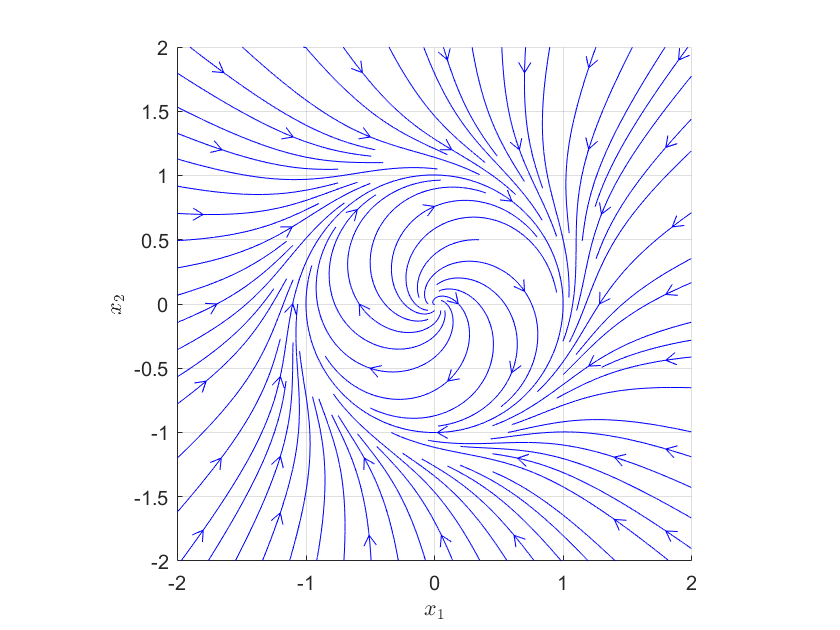
\includegraphics{images/cycle_limite.png}
\caption{Portrait de phase de l'exercice Cycle Limite
I}\label{fig_cycle_limite}
}
\end{figure}

\hypertarget{correc_lyap}{%
\section{Critères de stabilité de Lyapunov}\label{correc_lyap}}

\hypertarget{answer-lyap-1}{%
\subsubsection*{Question 1}\label{answer-lyap-1}}

\addcontentsline{toc}{subsubsection}{Question 1}

Supposons d'abord que \(\langle\nabla V (x), f(x)\rangle \leq 0\) pour
tout \(x\in W\). On a donc pour toute solution \(t\mapsto x(t)\)
initialisée dans \(W\), \(V(x(t))\leq V(x(0))\) tant que \(x(t)\in W\).
Prenons \(\varepsilon>0\) suffisamment petit tel que
\(B_f(a,2\varepsilon)\subset W\). On veut montrer qu'il existe \(\eta\)
tel que toute trajectoire initialisée dans \(B(a,\eta)\) reste dans
\(B(a,\varepsilon)\subset W\). Tout d'abord, il existe
\(\varepsilon_V>0\) tel que \[
\forall x\in B_f(a,2\varepsilon) \ : \ V(x)\leq \varepsilon_V \ \Longrightarrow x\in B(a,\varepsilon) \ .
\] En effet, sinon, il existerait une suite \((x_k)_{k\in \mathbb{N}}\)
d'éléments de \(B_f(a,2\varepsilon)\) telle que pour tout \(k>0\),
\(V(x_k)\leq \frac{1}{k}\) et \(\|x_k-a\|\geq \varepsilon\). L'ensemble
\(B_f(a,2\varepsilon)\) étant compact, on peut en extraire une
sous-suite convergeant vers \(x^\star\) qui vérifie nécessairement
\(V(x^\star)=0\) par continuité de \(V\) et
\(\|x^\star-a\|\geq \varepsilon\), i.e.~\(x^\star \neq a\). Ceci est
impossible par hypothèse. On a donc l'existence de \(\varepsilon_V\).
Maintenant, par continuité de \(V\) en \(a\) et puisque \(V(a)=0\), il
existe aussi \(\eta>0\) tel que \[
x\in B(a,\eta)  \ \Longrightarrow V(x)\leq \varepsilon_V \ .
\] Soit alors une solution maximale \(x\) avec \(x(0)\in B(a,\eta)\).
Attention, la décroissance de \(V(x(t))\) n'est acquise que tant que
\(x(t)\in W\)\,: il faut donc s'assurer que la solution ne quitte pas
\(W\). Supposons par l'absurde que \(x\) sorte de
\(B_f(a,2\varepsilon)\), et notons \[
t_1=\inf\{t\geq 0 \ : \ \|x(t)-a\|> 2\varepsilon\} >0 \ .
\] Sur \([0,t_1]\), \(x(t)\in B_f(a,2\varepsilon)\subset W\), donc
\(V(x(t))\leq V(x(0))\leq \varepsilon_V\) et ainsi
\(x(t)\in B(a,\varepsilon)\)\,; en particulier \(\|x(t_1)-a\|<\varepsilon\),
alors que par continuité et définition de \(t_1\),
\(\|x(t_1)-a\|=2\varepsilon\)~: contradiction. Donc \(x(t)\) reste dans
\(B_f(a,2\varepsilon)\subset W\), et le même argument donne
\(x(t)\in B(a,\varepsilon)\) pour tout \(t\geq 0\) tant qu'elle est
définie. Elle reste ainsi dans un compact de \(X\), donc par le
\protect\hyperlink{theo_bouts}{théorème du domaine maximal d'existence
(p. \pageref*{theo_bouts})}, \(x\) est définie sur
\(\mathbb{R}_{\geq 0}\). Ceci prouve la stabilité de \(a\).

\hypertarget{answer-lyap-2}{%
\subsubsection*{Question 2}\label{answer-lyap-2}}

\addcontentsline{toc}{subsubsection}{Question 2}

Supposons maintenant \(\langle\nabla V (x), f(x)\rangle < 0\) pour tout
\(x\in W\setminus \{a\}\). Alors par le point précédent \(a\) est
stable. Il suffit de montrer l'attractivité locale. Par stabilité, si
\(x(0)\in B(a,\eta)\), \(x(t)\in B(a,\varepsilon)\subset W\) pour tout
\(t\) et \(t\to V(x(t))\) est donc strictement décroissante. Comme elle
est aussi bornée inférieurement par 0, elle converge vers
\(\ell \geq 0\). Supposons \(\ell>0\). Alors, par continuité de \(V\),
il existe \(0<\nu<\varepsilon\) et \(\overline{t}>0\) tel que pour tout
\(t\geq \overline{t}\), \(\|x(t)-a\| \geq \nu\). Soit \[
\gamma = \max_{\nu \leq \|x-a\| \leq \varepsilon} \langle\nabla V (x), f(x)\rangle   
\] qui existe par continuité de \(\nabla V\) et \(f\) sur un compact.
Puisque \(\langle\nabla V (x), f(x)\rangle < 0\) sur
\(W\setminus \{a\}\), \(\gamma<0\). Alors, pour tout
\(t\geq \overline{t}\), \[
V(x(t)) = V(x(\overline{t})) + \int_{\overline{t}}^t \langle\nabla V (x(s)), f(x(s))\rangle ds \leq  V(x(\overline{t})) + \gamma (t-\overline{t}) \ .
\] Mais comme \(\gamma<0\) cette quantité devient strictement négative
au bout d'un certain temps, ce qui est impossible. Donc
\(\lim_{t\to +\infty} V(x(t))=0\). Finalement, reproduisant le même
raisonnement que pour l'existence de \(\varepsilon_V\), on peut garantir
que \(\|x-a\|\) est arbitrairement petit en prenant \(V(x)\)
suffisamment petit. Donc on en déduit que
\(\lim_{t\to +\infty} \|x(t)-a\|=0\).

\hypertarget{answer-lyap-3}{%
\subsubsection*{Question 3}\label{answer-lyap-3}}

\addcontentsline{toc}{subsubsection}{Question 3}

Supposons enfin que \(\lim_{\|x\|\to +\infty} V(x) = +\infty\) et
\(W=\mathbb{R}^n\). Alors \(V(x(t))\leq V(x(0))\) pour tout \(t\in I\), \(t\geq 0\), donc
\(x(t)\in V^{-1}(\left[ 0,V(x(0)) \right])\) pour tout \(t\geq 0\). Le fait
que \(\lim_{\|x\|\to +\infty} V(x) = +\infty\) est équivalent au fait
que l'image réciproque de toute compact est compact (on dit que \(V\)
est propre). Donc \(V^{-1}(\left[ 0,V(x(0)) \right])\) est compact et
par le \protect\hyperlink{theo_bouts}{théorème du domaine maximal
d'existence nécessairement (p. \pageref*{theo_bouts})} \(x(t)\) est
défini pour tout \(t\geq 0\), et reste dans ce compact. Alors on peut
reproduire le même raisonnement que plus haut et obtenir la convergence
de \(x\) vers \(a\).

\hypertarget{answer-lyap-4}{%
\subsubsection*{Question 4 (Application à la stabilité des systèmes
linéaires)}\label{answer-lyap-4}}

\addcontentsline{toc}{subsubsection}{Question 4 (Application à la stabilité des systèmes linéaires)}

Puisque les valeurs propres de \(A\) sont à partie réelle strictement
négative, il existe \(C\geq 1\) et \(\mu>0\) tels que
\(\|e^{As}\|\leq C e^{-\mu s}\) pour tout \(s\geq 0\). L'intégrale \[
P=\int_0^{+\infty}\left(e^{As}\right)^\top Q e^{As}ds
\] est donc bien définie (absolument convergente). La matrice \(P\) est
symétrique car l'intégrande l'est. Pour tout \(x\in\mathbb{R}^n\), \[
x^\top P x = \int_0^{+\infty}\left(e^{As}x\right)^\top Q \left(e^{As}x\right)ds
\geq \lambda_{\min}(Q)\int_0^{+\infty}\|e^{As}x\|^2 ds \ ,
\] qui est strictement positif si \(x\neq 0\) car \(e^{As}\) est
inversible et \(s\mapsto \|e^{As}x\|^2\) est continue. Donc \(P\) est
définie positive. Enfin, puisque \(A\) commute avec \(e^{As}\), \[
A^\top P + PA = \int_0^{+\infty}\left( A^\top e^{A^\top s} Q e^{As} + e^{A^\top s} Q e^{As} A \right) ds
= \int_0^{+\infty}\frac{d}{ds}\left( e^{A^\top s} Q e^{As} \right) ds
= \lim_{S\to+\infty} e^{A^\top S} Q e^{AS} - Q = -Q \ ,
\] car \(\|e^{AS}\|\to 0\) lorsque \(S\to +\infty\).

Posons alors \(V(x)=x^\top P x\). Cette fonction est \(C^1\), \(V(0)=0\),
\(V(x)>0\) pour \(x\neq 0\), et
\(V(x)\geq \lambda_{\min}(P)\|x\|^2\to+\infty\) lorsque
\(\|x\|\to+\infty\). De plus, pour tout \(x\), \[
\langle \nabla V(x), Ax\rangle = 2x^\top P A x = x^\top\left(A^\top P + PA\right)x = -x^\top Q x < 0 \qquad \forall x\neq 0 \ .
\] Par la question 3 (avec \(f(x)=Ax\), \(a=0\), \(W=\mathbb{R}^n\)), \(0\)
est globalement asymptotiquement stable pour \(\dot{x}=Ax\).

\hypertarget{answer-lyap-5}{%
\subsubsection*{Question 5 (Application à la stabilité via linéarisé
tangent)}\label{answer-lyap-5}}

\addcontentsline{toc}{subsubsection}{Question 5 (Application à la stabilité via linéarisé tangent)}

Posons \(J=J_f(a)\) et \[
\Delta(x) = f(x)-f(a) - J(x-a) = f(x)- J(x-a)\ ,
\] puisque \(f(a)=0\). Par différentiabilité de \(f\) en \(a\), la
fonction \(\delta\) définie par \(\delta(x)=\Delta(x)/\|x-a\|\) pour
\(x\neq a\) et \(\delta(a)=0\) vérifie \(\lim_{x\to a}\delta(x)=0\), et
\(\Delta(x)=\delta(x)\|x-a\|\) pour tout \(x\).

Par la question 4 avec \(A=J\) et \(Q=I\), il existe \(P=P^\top>0\) telle
que \[
J^\top P +P J = -I \ .
\] Considérons \(V(x) = (x-a)^\top P (x-a)\), qui est \(C^1\), positive
et nulle seulement en \(x=a\). Pour tout \(x\in X\), \begin{align*}
\left< \nabla V(x), f(x) \right> & = 2(x-a)^\top P f(x) \\
&= (x-a)^\top\left( J^\top P +P J\right) (x-a) + 2 (x-a)^\top P\Delta(x) \\
&\leq - \|x-a\|^2 + 2 \|x-a\| \|P\| \|\Delta(x)\| \\
&\leq - \|x-a\|^2\left(1- 2\|P\|  \|\delta(x) \| \right) \ .
\end{align*} Comme \(X\) est ouvert et \(\delta(x)\to 0\) lorsque
\(x\to a\), il existe \(r>0\) tel que \(B(a,r)\subset X\) et \[
\|\delta(x) \| \leq  \frac{1}{4\|P\|}  \qquad \forall x\in B(a,r) \ .
\] Alors \(\left< \nabla V(x), f(x) \right> \leq -\frac{1}{2}\|x-a\|^2 <0\)
pour tout \(x\in B(a,r)\setminus\{a\}\). Par la question 2 (avec
\(W=B(a,r)\)), \(a\) est localement asymptotiquement stable.

\hypertarget{correc_instab}{%
\section{Critères d'instabilité}\label{correc_instab}}

\hypertarget{answer-instab-1}{%
\subsubsection*{Question 1 (Théorème de Chetaev)}\label{answer-instab-1}}

\addcontentsline{toc}{subsubsection}{Question 1 (Théorème de Chetaev)}

Supposons par l'absurde que \(a\) soit stable. Prenons
\(\varepsilon>0\) tel que \(B_f(a,\varepsilon)\subset W\). Par
stabilité, il existe \(\eta>0\) tel que toute solution maximale
initialisée dans \(B_f(a,\eta)\) est définie sur
\(\mathbb{R}_{\geq 0}\) et reste dans \(B_f(a,\varepsilon)\). Par
hypothèse, il existe \(x_0\in B(a,\eta)\) tel que \(V(x_0)>0\). Soit
\(x\) une solution maximale initialisée en \(x_0\) et
\(v(t)=V(x(t))\), qui est \(C^1\) sur \(\mathbb{R}_{\geq 0}\) avec \[
\dot{v}(t) = \langle\nabla V (x(t)), f(x(t))\rangle \ .
\] Montrons d'abord que \(v(t)\geq v(0)\) pour tout \(t\geq 0\). Sinon,
\(t_1 = \inf\{t\geq 0 \ : \ v(t)<v(0)\}\) vérifie \(v(t_1)=v(0)>0\) par
continuité, donc \(\dot{v}(t_1)>0\) par hypothèse, et \(v>v(0)\) sur un
intervalle \(]t_1,t_1+h]\), ce qui contredit la définition de \(t_1\).
Ainsi, pour tout \(t\geq 0\), \(x(t)\) appartient à \[
K = \left\{ x\in B_f(a,\varepsilon) \ : \ V(x)\geq V(x_0) \right\} \ ,
\] qui est compact (fermé dans le compact \(B_f(a,\varepsilon)\) par
continuité de \(V\)) et ne contient pas \(a\) puisque \(V(a)=0<V(x_0)\).
Soit \[
\gamma = \min_{x\in K} \langle\nabla V (x), f(x)\rangle
\] qui existe par continuité de \(\nabla V\) et \(f\) sur le compact
\(K\). Puisque \(V>0\) sur \(K\), \(\gamma>0\) par hypothèse. Alors,
pour tout \(t\geq 0\), \[
V(x(t)) = V(x_0) + \int_0^t \langle\nabla V (x(s)), f(x(s))\rangle ds \geq V(x_0) + \gamma t \ ,
\] qui tend vers \(+\infty\). C'est impossible puisque \(V\) est
continue donc bornée sur le compact \(B_f(a,\varepsilon)\). Donc \(a\)
est instable.

\hypertarget{answer-instab-2}{%
\subsubsection*{Question 2 (Exemples)}\label{answer-instab-2}}

\addcontentsline{toc}{subsubsection}{Question 2 (Exemples)}

Pour \(\dot{x}=x^3\), prenons \(V(x)=x^2\), qui est \(C^1\), nulle en
\(0\) et strictement positive ailleurs. On a
\(\langle\nabla V (x), x^3\rangle = 2x^4 >0\) pour tout \(x\neq 0\), donc
\(0\) est instable par la question 1 avec \(W=\mathbb{R}\). Notons que
le \protect\hyperlink{theo_linTangent}{théorème du linéarisé tangent (p.
\pageref*{theo_linTangent})} ne permet pas de conclure ici puisque le
linéarisé en \(0\) est nul. On peut d'ailleurs vérifier que la solution
initialisée en \(x_0\neq 0\) est
\(x(t)=\frac{x_0}{\sqrt{1-2x_0^2 t}}\), qui explose en temps fini
\(t=\frac{1}{2x_0^2}\), aussi proche de \(0\) que soit \(x_0\).

Pour le second système, prenons \(V(x)=x_1^2-x_2^2\), qui n'est pas de
signe constant. On a \(V(0)=0\), \(V(\eta,0)=\eta^2>0\) pour tout
\(\eta>0\), et \[
\langle\nabla V (x), f(x)\rangle = 2x_1\cdot x_1 - 2x_2\cdot(-x_2) = 2\|x\|^2 >0 \qquad \forall x\neq 0 \ ,
\] en particulier lorsque \(V(x)>0\). Par la question 1 avec
\(W=\mathbb{R}^2\), \(0\) est instable. Les trajectoires s'éloignent en
effet de \(0\) selon la direction \(x_1\)~: c'est un \emph{point selle}.

\hypertarget{answer-instab-3}{%
\subsubsection*{Question 3 (Application à l'instabilité des systèmes
linéaires)}\label{answer-instab-3}}

\addcontentsline{toc}{subsubsection}{Question 3 (Application à l'instabilité des systèmes linéaires)}

Notons \(\lambda_1,\ldots,\lambda_p\) les valeurs propres (complexes,
distinctes) de \(A\), de multiplicités \(m_1,\ldots,m_p\), et
\(\mu = \max_i \mathrm{Re}(\lambda_i)>0\). Choisissons
\(\sigma\in \, ]0,\mu[\) différent de tous les \(\mathrm{Re}(\lambda_i)\),
ce qui est possible puisqu'ils sont en nombre fini. Ce décalage permet
de traiter les éventuelles valeurs propres de partie réelle nulle, qui
ne sont ni \og stables\fg{} ni \og instables\fg{}~: elles sont ici rangées
du côté stable.

Écrivons le polynôme caractéristique \(\chi_A=\chi_+\chi_-\), où
\(\chi_+\) (resp. \(\chi_-\)) est le produit des facteurs
\((X-\lambda_i)^{m_i}\) tels que \(\mathrm{Re}(\lambda_i)>\sigma\) (resp.
\(\mathrm{Re}(\lambda_i)<\sigma\)). Les valeurs propres non réelles de
\(A\) étant deux à deux conjuguées avec la même multiplicité, \(\chi_+\)
et \(\chi_-\) sont à coefficients réels, et ils sont premiers entre eux.
Par le théorème de Cayley-Hamilton et le lemme des noyaux, \[
\mathbb{R}^n = E_+ \oplus E_- \qquad , \qquad E_\pm = \ker \chi_\pm(A) \ ,
\] où \(E_+\) et \(E_-\) (éventuellement réduit à \(\{0\}\)) sont stables
par \(A\). Il existe donc \(T\in \mathbb{R}^{n\times n}\) inversible
(dont les colonnes sont une base de \(E_+\) suivie d'une base de
\(E_-\)) telle que \[
T^{-1}AT = \left( \begin{matrix} A_+ & 0\\ 0 & A_- \end{matrix}\right) \ ,
\] où \(\chi_\pm(A_\pm)=0\). Les valeurs propres de \(A_+\) sont donc des
racines de \(\chi_+\), c'est-à-dire de partie réelle \(>\sigma\), et
celles de \(A_-\) sont de partie réelle \(<\sigma\). Par ailleurs,
\(E_+\neq\{0\}\)~: si \(v\in\mathbb{C}^n\) est un vecteur propre associé
à une valeur propre \(\lambda\) de partie réelle \(\mu\), alors
\(\chi_+(A)v = \chi_+(\lambda)v = 0\), donc \(\mathrm{Re}(v)\) et
\(\mathrm{Im}(v)\), qui ne sont pas tous deux nuls, sont dans \(E_+\)
puisque \(\chi_+(A)\) est réelle.

Les valeurs propres de \(\sigma I-A_+\) et de \(A_- - \sigma I\) sont
donc toutes à partie réelle strictement négative. Par la
\protect\hyperlink{lyap-4}{question 4 de l'exercice \emph{Critères de
stabilité de Lyapunov} (p. \pageref*{lyap-4})} appliquée avec
\(Q=I\), il existe \(P_+\) et \(P_-\) symétriques définies positives
telles que \[
(\sigma I-A_+)^\top P_+ + P_+(\sigma I-A_+) = -I \qquad , \qquad (A_- -\sigma I)^\top P_- + P_-(A_- -\sigma I) = -I \ ,
\] c'est-à-dire \[
A_+^\top P_+ + P_+A_+ = 2\sigma P_+ + I \qquad , \qquad A_-^\top P_- + P_-A_- = 2\sigma P_- - I \ .
\] Posons alors, avec \(T^{-\top}=(T^{-1})^\top\), \[
D = \left( \begin{matrix} P_+ & 0\\ 0 & -P_- \end{matrix}\right) \qquad , \qquad P = T^{-\top} D\, T^{-1} \qquad , \qquad Q = T^{-\top} T^{-1} \ .
\] Les matrices \(P\) et \(Q\) sont symétriques, \(Q\) est définie
positive, et en notant \(M=T^{-1}AT\), \begin{align*}
A^\top P + PA &= T^{-\top}\left( M^\top D + D M\right) T^{-1} \\
&= T^{-\top} \left( \begin{matrix} A_+^\top P_+ + P_+A_+ & 0\\ 0 & -(A_-^\top P_- + P_-A_-) \end{matrix}\right) T^{-1} \\
&= T^{-\top} \left( 2\sigma D + I \right) T^{-1} = 2\sigma P + Q \ .
\end{align*} Enfin, pour \(z_+\in\mathbb{R}^{\dim E_+}\) non nul et
\(\bar{x} = T(z_+,0)\), on a \(\bar{x}^\top P \bar{x} = z_+^\top P_+ z_+>0\).

Considérons maintenant \(V(x)=x^\top P x\). On a \(V(0)=0\) et, pour
tout \(t>0\), \(V(t\bar{x}) = t^2\,\bar{x}^\top P \bar{x}>0\), donc
\(V\) prend des valeurs strictement positives arbitrairement près de
\(0\). De plus, pour tout \(x\in\mathbb{R}^n\), \[
\langle\nabla V (x), Ax\rangle = 2x^\top PAx = x^\top\left(A^\top P + PA\right) x = 2\sigma V(x) + x^\top Q x \ ,
\] qui est strictement positif dès que \(V(x)>0\) (et donc
\(x\neq 0\)). Par la question 1 avec \(W=\mathbb{R}^n\), \(0\) est
instable pour \(\dot{x}=Ax\).

Notons que pour un système linéaire, on pouvait conclure plus
directement~: si \(v\) est un vecteur propre associé à une valeur propre
\(\lambda\) de partie réelle strictement positive, la solution
initialisée en \(\eta\,\mathrm{Re}(v)\) s'écrit
\(x(t)=\eta\,\mathrm{Re}(e^{\lambda t}v)\) et n'est pas bornée, aussi
petit que soit \(\eta>0\). L'intérêt de la fonction \(V\) construite
ici est qu'elle reste une fonction de Chetaev pour des perturbations non
linéaires de \(\dot{x}=Ax\), comme on va le voir à la question suivante.

\hypertarget{answer-instab-4}{%
\subsubsection*{Question 4 (Application à l'instabilité via linéarisé
tangent)}\label{answer-instab-4}}

\addcontentsline{toc}{subsubsection}{Question 4 (Application à l'instabilité via linéarisé tangent)}

Comme dans la \protect\hyperlink{answer-lyap-5}{question 5 de l'exercice
\emph{Critères de stabilité de Lyapunov} (p. \pageref*{answer-lyap-5})},
posons \(J=J_f(a)\) et \(\Delta(x) = f(x) - J(x-a)\), de sorte que
\(\Delta(x)=\delta(x)\|x-a\|\) avec \(\lim_{x\to a}\delta(x)=0\). Par la
question 3 appliquée à \(A=J\), il existe \(\sigma>0\), \(Q\) symétrique
définie positive et \(P\) symétrique telles que \[
J^\top P + PJ = 2\sigma P + Q \ ,
\] et \(\bar{x}\in\mathbb{R}^n\) tel que \(\bar{x}^\top P \bar{x}>0\)
(en particulier \(P\neq 0\)). Considérons
\(V(x) = (x-a)^\top P (x-a)\). Pour tout \(x\in X\), \begin{align*}
\left< \nabla V(x), f(x) \right> & = 2(x-a)^\top P f(x) \\
&= (x-a)^\top\left( J^\top P +P J\right) (x-a) + 2 (x-a)^\top P\Delta(x) \\
&= 2\sigma V(x) + (x-a)^\top Q (x-a) + 2 (x-a)^\top P\Delta(x) \\
&\geq 2\sigma V(x) + \lambda_{\min}(Q)\|x-a\|^2 - 2 \|P\|  \|\delta(x) \| \|x-a\|^2 \ .
\end{align*} Comme \(X\) est ouvert et \(\delta(x)\to 0\) lorsque
\(x\to a\), il existe \(r>0\) tel que \(B(a,r)\subset X\) et \[
\|\delta(x) \| \leq  \frac{\lambda_{\min}(Q)}{4\|P\|}  \qquad \forall x\in B(a,r) \ .
\] Alors, pour tout \(x\in B(a,r)\), \[
\left< \nabla V(x), f(x) \right> \geq 2\sigma V(x) + \frac{\lambda_{\min}(Q)}{2}\|x-a\|^2 \ ,
\] qui est strictement positif dès que \(V(x)>0\) (et donc \(x\neq a\)).
Par ailleurs \(V(a)=0\) et \(V(a+t\bar{x}) = t^2\,\bar{x}^\top P \bar{x}>0\)
pour tout \(t>0\), avec \(a+t\bar{x}\in B(a,r)\) pour \(t\) assez
petit. Par la question 1 avec \(W=B(a,r)\), \(a\) est instable.

\hypertarget{correc_cycle_lim_volterra}{%
\section{Cycle limite II}\label{correc_cycle_lim_volterra}}

On étudie le comportement des solutions de \(\dot{x}=f(x)\) pour \[
f(x) = 
\left(
\begin{matrix}
x_1(\alpha -\beta x_2)  \\
-x_2(\gamma-\delta x_1)
\end{matrix}
\right)
\]

\hypertarget{answer-cycle-lim-volterra-1}{%
\subsubsection*{Question 1}\label{answer-cycle-lim-volterra-1}}

\addcontentsline{toc}{subsubsection}{Question 1}

On résout \(f(x) = 0\), ce qui donne les points d'équilibre \((0,0)\) et
\(\bar{x}=\left(\frac{\gamma}{\delta},\frac{\alpha}{\beta} \right)\).

La jacobienne de la dynamique est donnée par \[
J_f(x) = 
\left(
\begin{matrix}
\alpha -\beta x_2 & -\beta x_1 \\
\delta x_2 & -(\gamma-\delta x_1)
\end{matrix}
\right)
\] En \((0,0)\), \[
J_f(0,0) = 
\left(
\begin{matrix}
\alpha & 0 \\
0 & -\gamma
\end{matrix}
\right)
\] a pour valeur propre \(\alpha>0\), donc \((0,0)\) est instable. Par
contre, en \(\bar{x}\), \[
J_f(\bar{x}) = 
\left(
\begin{matrix}
0 & -\beta\frac{\gamma}{\delta} \\
\delta\frac{\alpha}{\beta} & 0
\end{matrix}
\right)
\] a des valeurs propres imaginaires pures \(\pm i\sqrt{\alpha\gamma}\),
donc a priori on ne peut rien dire sur la stabilité de \(\bar{x}\) pour le système
non linéaire.

\hypertarget{answer-cycle-lim-volterra-2}{%
\subsubsection*{Question 2}\label{answer-cycle-lim-volterra-2}}

\addcontentsline{toc}{subsubsection}{Question 2}

Soit \(x_0=(0,x_{2,0})\in \{0\}\times \mathbb{R}_{\geq 0}\) sur l'axe
des ordonnées. Puisque \(f\) est \(C^1\) sur \(\mathbb{R}^2\), par le
théorème de Cauchy-Lipschitz, le problème de Cauchy associé à la
condition initiale \((t_0,x_0)\) pour un \(t_0\) quelconque, admet une
unique solution \[
x(t) = (0, x_2(t))
\] définie sur \(\mathbb{R}\) avec \(x_2\) solution de \[
\dot{x}_2 = -\gamma x_2 \ .
\]

De même, pour \(x_0=(x_{1,0},0)\in \mathbb{R}_{\geq 0}\times \{0\}\), le
problème de Cauchy associé pour un \(t_0\) quelconque, admet une unique
solution du type \[
x(t) = (x_1(t), 0)
\] définie sur \(\mathbb{R}\) avec \(x_1\) solution de \[
\dot{x}_1 = \alpha x_1 \ .
\]

Si une solution initialisée dans
\(\mathbb{R}_{>0}\times\mathbb{R}_{>0}\) croisait l'axe des abscisses ou
des ordonnées, il existerait une autre solution au problème de Cauchy
associé à \(x_0=(0,x_{2,0})\) ou \(x_0=(x_{1,0},0)\) qui ne resterait
pas sur l'axe en temps négatif, ce qui est impossible. Elle reste donc
dans \(\mathbb{R}_{>0}\times\mathbb{R}_{>0}\).

\hypertarget{answer-cycle-lim-volterra-3}{%
\subsubsection*{Question 3}\label{answer-cycle-lim-volterra-3}}

\addcontentsline{toc}{subsubsection}{Question 3}

\(f\) est continue sur \(\mathbb{R}^2\) donc d'après le
théorème du domaine maximal d'existence, si une solution maximale
initialisée dans \(\mathbb{R}^2\) n'est pas définie sur
\(\mathbb{R}\), c'est que nécessairement \(\|x\|\) diverge en temps fini
(car la frontière de \(\mathbb{R}^2\) est vide).

Maintenant considérons une solution maximale
\(x:I\subset \mathbb{R} \to \mathbb{R}^2\) initialisée dans
\(\mathbb{R}_{>0}\times\mathbb{R}_{>0}\). Par la question précédente,
elle reste dans \(\mathbb{R}_{>0}\times\mathbb{R}_{>0}\) donc
\(H(x(t))\) est bien définie pour tout \(t\in I\), et on a \[
\frac{d}{dt}H(x(t)) = \langle \nabla H(x(t)) , \dot{x}(t) \rangle =  \langle \nabla H(x(t)) , f(x(t)) \rangle =0
\] Donc \(H\) est constante et il est impossible que \(\|x\|\) diverge
en temps fini car on aurait \(\lim H(x(t)) = +\infty\). Donc
\(I=\mathbb{R}\).

\emph{Remarque}~: On aurait pu aussi directement se placer sur
\(\mathbb{R}_{>0}\times\mathbb{R}_{>0}\) et considérer les solutions
maximales
\(x:I\subset \mathbb{R} \to \mathbb{R}_{>0}\times\mathbb{R}_{>0}\) de
\(\dot{x}=f(x)\) dans cet ensemble (où \(f\) est bien sûr continue). Si
\(x\) n'était pas définie sur \(\mathbb{R}\), alors nécessairement
d'après le théorème du domaine maximal d'existence, \(x(t)\) finirait,
en temps fini, par être à chaque instant soit arbitrairement loin de
l'origine, soit arbitrairement proche de la frontière de
\(\mathbb{R}_{>0}\times\mathbb{R}_{>0}\), c'est-à-dire avec \(x_1\) ou
\(x_2\) arbitrairement petit. Mais ceci est impossible car
\(H(x) = u_{\delta,\gamma}(x_1) + u_{\beta,\alpha}(x_2)\), où
\(u_{c,d}(z) = cz - d\ln z\) est minorée et tend vers \(+\infty\) en
\(0^+\) comme en \(+\infty\)~: dans chacun des cas on aurait \[
\lim H(x(t)) = +\infty \ ,
\] contredisant la conservation de \(H\). On prouve alors en même temps que les solutions initialisées dans
\(\mathbb{R}_{>0}\times\mathbb{R}_{>0}\) sont définies sur
\(\mathbb{R}\) dans \(\mathbb{R}_{>0}\times\mathbb{R}_{>0}\) (et donc
restent dans cet ensemble)

\emph{Bonus}~: Ici, en calculant le gradient et la hessienne de \(H\)
(voir Calcul Différentiel III), on voit que \(H\) atteint un minimum
local (et en fait global) en \(\bar{x}\) (gradient nul et matrice
hessienne définie positive, mais on peut aussi le montrer en étudiant la
fonction réelle \(u(z)=z-c\ln z\) pour une constante \(c>0\)). Donc
\[
V(x) = H(x)-H(\bar{x})
\] est une fonction \(C^1\) sur
\(\mathbb{R}_{>0}\times\mathbb{R}_{>0}\), positive, qui ne s'annule
localement qu'en \(\bar{x}\). Vu que \(H\) est conservée le long des
trajectoires, on peut déduire que \(\bar{x}\) est stable par le
\protect\hyperlink{stab_decroissance}{théorème de décroissance (p.
\pageref*{stab_decroissance})}.

\hypertarget{answer-cycle-lim-volterra-4}{%
\subsubsection*{Question 4}\label{answer-cycle-lim-volterra-4}}

\addcontentsline{toc}{subsubsection}{Question 4}

L'équilibre \(\bar{x}\) se trouve au milieu des courbes de niveau (car
c'est en fait le minimum de \(H\)). Donc si on se donne
\(\varepsilon >0\), on peut trouver \(\eta_H>0\) tel que \(H(x)-H(\bar{x})<\eta_H\)
implique \(\|x-\bar{x}\|<\varepsilon\). On en déduit que pour toute
condition initiale telle que \(H(x_0)-H(\bar{x})<\eta_H\), la trajectoire reste à
une distance inférieure à \(\varepsilon\) de \(\bar{x}\). Par ailleurs,
l'ensemble des courbes de niveau de \(H-H(\bar{x})\) inférieures à \(\eta_H\)
constituent bien un voisinage de \(\bar{x}\) donc \(\bar{x}\) est stable
par définition.

Le portrait de phase est donné
\protect\hyperlink{fig_cycle_limiteII}{Figure~\ref*{fig_cycle_limiteII} (p.
\pageref*{fig_cycle_limiteII})}.

\begin{figure}
\hypertarget{fig_cycle_limiteII}{%
\centering
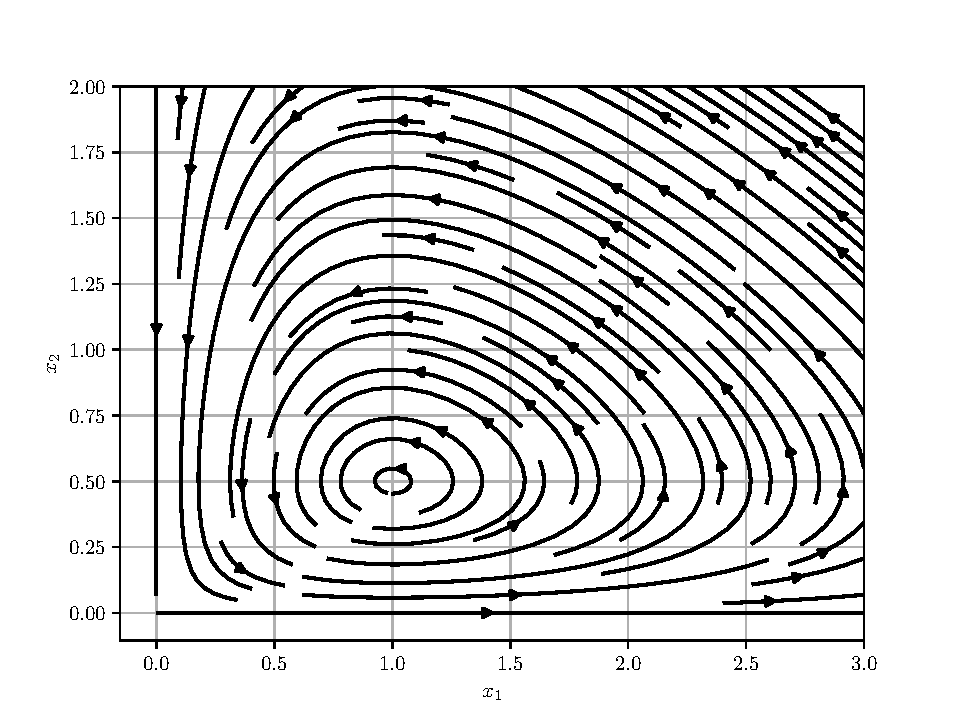
\includegraphics{images/cycle_limiteII.py.pdf}
\caption{Portrait de phase de l'exercice Cycle Limite
II}\label{fig_cycle_limiteII}
}
\end{figure}

\hypertarget{answer-cycle-lim-volterra-5}{%
\subsubsection*{Question 5}\label{answer-cycle-lim-volterra-5}}

\addcontentsline{toc}{subsubsection}{Question 5}

Pour que \(x_1\) vale \(x_1^*\) à l'équilibre, il faut que \(x_2\) vale
\(x_2^* = \frac{\alpha}{\beta}\) et
\(u^* = x_2^*(\gamma-\delta x_1^*)\).

\hypertarget{answer-cycle-lim-volterra-6}{%
\subsubsection*{Question 6}\label{answer-cycle-lim-volterra-6}}

\addcontentsline{toc}{subsubsection}{Question 6}

Commençons par justifier le choix de la référence \(v_r\). Si l'on
parvenait à imposer \(x_2 = v_r(x_1)\), la première équation deviendrait
\[
\dot{x}_1 = x_1\big(\alpha - \beta v_r(x_1)\big) = -\beta\lambda_1\, x_1 (x_1-x_1^*) \ ,
\] équation scalaire pour laquelle \(x_1^*\) est asymptotiquement stable
sur \(\mathbb{R}_{>0}\) (\(\dot{x}_1<0\) si \(x_1>x_1^*\), \(\dot{x}_1>0\)
si \(0<x_1<x_1^*\)). La référence \(v_r(x_1)=\frac{\alpha}{\beta}+\lambda_1(x_1-x_1^*)\)
corrige donc la valeur d'équilibre \(\frac{\alpha}{\beta}\) des
prédateurs proportionnellement à l'écart des proies à leur cible\,:
plus de prédateurs s'il y a trop de proies, moins s'il n'y en a pas
assez. Il reste à faire converger \(x_2\) vers \(v_r(x_1)\) à l'aide de
\(u\), ce que mesure le second terme de \(V\).

On utilise ici pour simplifier le deuxième
\protect\hyperlink{exo_lyap}{critère de Lyapunov (p.
\pageref*{exo_lyap})}. La fonction \(V\) est \(C^1\), à valeurs
positives et s'annule si et seulement si \(x_1=x_1^*\) et
\(x_2 = v_r(x_1^*)=x_2^*\). C'est donc une fonction de Lyapunov associée à
\((x_1^*,x_2^*)\). Calculons sa dérivée le long des trajectoires.
\begin{multline*}
\langle \nabla V(x) , f(x) \rangle = -2\beta\lambda_1 x_1(x_1-x_1^*)^2 -2\beta x_1(x_1-x_1^*)(x_2-v_r(x_1)) \\
+ 2(x_2-v_r(x_1))\left(-x_2(\gamma-\delta x_1)+u - \lambda_1 f_1(x) \right)
\end{multline*} en utilisant \(\alpha-\beta x_2 = -\beta\lambda_1(x_1-x_1^*) - \beta(x_2-v_r(x_1))\)
et \(\frac{d}{dt}\left(x_2-v_r(x_1)\right) = \dot{x}_2 - v_r'(x_1)\dot{x}_1 = \dot{x}_2 - \lambda_1 f_1(x)\).
L'idée est alors de choisir \(u\) afin d'assurer que
\(\langle \nabla V(x) , f(x) \rangle< 0\) au moins dans un voisinage de
l'équilibre. On prend donc par exemple \[
u =  -\lambda_2(x_2-v_r(x_1)) + x_2(\gamma-\delta x_1) + \lambda_1f_1(x) + \beta x_1(x_1-x_1^*)
\] avec \(\lambda_2>0\). Ceci donne \[
\langle \nabla V(x) , f(x) \rangle = -2\beta\lambda_1 x_1(x_1-x_1^*)^2 -2\lambda_2(x_2-v_r(x_1))^2
\] qui est bien strictement négatif pour \(x\neq (x_1^*,x_2^*)\) dans un
voisinage où \(x_1>0\). On en déduit que \((x_1^*,x_2^*)\) est
localement asymptotiquement stable. Il ne l'est pas globalement car
\((0,v_r(0))=(0,\frac{\alpha}{\beta}-\lambda_1 x_1^*)\) est aussi point d'équilibre
du système bouclé (en \(x_1=0\), on a \(\dot x_2 = -\lambda_2(x_2-v_r(0))\)). Mais ce dernier est instable
(\(\frac{\partial f_1}{\partial x_1}(0,v_r(0)) = \beta\lambda_1 x_1^*>0\))
et une étude plus fine pourrait montrer que le bassin d'attraction
inclut \(\mathbb{R}_{> 0}\times\mathbb{R}_{> 0}\).

\begin{figure}
\hypertarget{fig_cycle_limiteII_control}{%
\centering
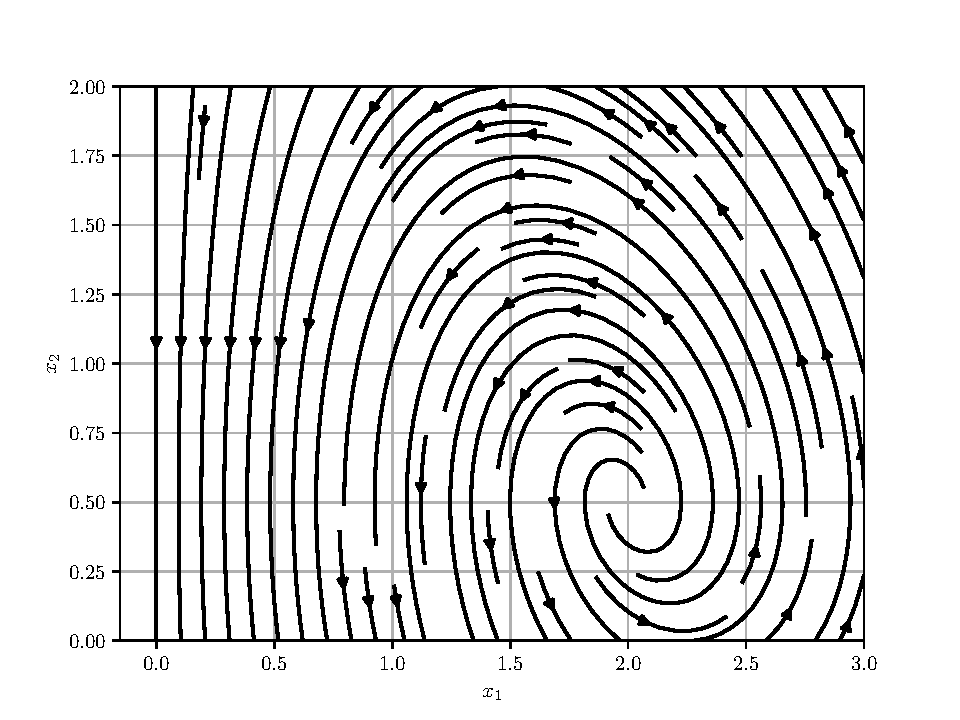
\includegraphics{images/cycle_limiteII_control.py.pdf}
\caption{Portrait de phase de l'exercice Cycle Limite II avec l'entrée
\(u\) choisie pour \(x_1^*=2\) avec
\(\lambda_1=\lambda_2=1\).}\label{fig_cycle_limiteII_control}
}
\end{figure}

\hypertarget{answer-attrac_stab}{%
\section{Attractivité locale implique stabilité asymptotique globale
pour un système linéaire}\label{answer-attrac_stab}}

Tout d'abord, montrons que l'attractivité locale de 0 implique
l'attractivité globale. Ceci est dû à la propriété d'\emph{homogénéité}
des systèmes linéaires: si \(x\) est une solution initialisée à
\(x_0\in\mathbb{R}\), alors \(\lambda x\) est solution initialisée à
\(\lambda x_0\) puisque \[
\lambda x(t) = \lambda e^{At} x_0 = e^{At} (\lambda x_0) \ .
\] Donc soit \(\eta>0\) tel que toute solution initialisée dans
\(B(0,\eta)\) converge vers 0. Soit \(x\) une solution initialisée à
\(x_0\in\mathbb{R}\). Alors \(\lambda x\) avec
\(\lambda < \eta / \|x_0\|\) est solution initialisée dans \(B(0,\eta)\)
et converge vers 0. Donc \(x\) converge vers 0.

Maintenant, montrons la stabilité. Soit \(\varepsilon >0\). Notons
\((x_i)_{i=1...n}\) une base orthonormale de \(\mathbb{R}^n\). Soit
alors \(M>0\) tel que \[
\|e^{At} x_i \| \leq M \quad \forall t \in \mathbb{R}_{\geq 0}\quad \forall i\in \{1,...,n\}
\] qui existe bien puisque toutes les solutions convergent vers 0 et
\(n\) est fini. Soit maintenant \(\eta >0\). Pour tout
\(x_0 \in B(0,\eta)\) dont la décomposition dans la base s'écrit \[
x_0 = \sum_{i=1}^n \alpha_i x_i
\] on a \(|\alpha_i|\leq \eta\) et donc pour tout
\(t \in \mathbb{R}_{\geq 0}\), \[
\left\| e^{At} x_0 \right\| \leq \left\| \sum_{i=1}^n  e^{At} \alpha_i x_i\right\|  \leq  n \eta M
\] On conclut que pour des conditions initiales suffisamment petites
(\(\eta <\frac{\varepsilon}{nM}\)), les solutions restent inférieures à
\(\varepsilon\) en norme. Donc le système est stable.

\hypertarget{correc_cont_lin}{%
\section{Stabilisation d'une chaîne
d'intégrateurs}\label{correc_cont_lin}}

La dynamique du système est de la forme \(\dot{x} = f(x,u)\).

\hypertarget{answer-cont-lin-1}{%
\subsubsection*{Question 1}\label{answer-cont-lin-1}}

\addcontentsline{toc}{subsubsection}{Question 1}

Pour que \(x^*\) soit point d'équilibre avec la commande \(u^*\), il
faut \(f(x^*,u^*)=0\), soit \(x_2^*=x_3^*=\ldots=x_n^*=0\) et
\(u^* = -\phi(x_1^*,0,\ldots,0)\).

\hypertarget{answer-cont-lin-2}{%
\subsubsection*{Question 2}\label{answer-cont-lin-2}}

\addcontentsline{toc}{subsubsection}{Question 2}

L'idée est de se placer autour de \(x^*\) et donc considérer l'erreur
\(e = x-x^*\) que l'on souhaite stabiliser à 0. On constate alors que \[
\begin{array}{rcl}
\dot{e}_1 &=& e_2 \\
\dot{e}_2 &=& e_3 \\
&\vdots&\\
\dot{e}_{n-1} &=& e_n \\
\dot{e}_n &=& \phi(x) + u(t)
\end{array}
\] Si l'on mesure \(x(t)\), on peut prendre \[
u(t) = -\phi(x(t)) -k_1 e_1(t) - k_2 e_2(t) - \ldots - k_n e_n(t)
\] ce qui donne \[
\dot{e} = A e
\] avec \(A\) de la forme \[
A = \left(
\begin{array}{ccccc}
0&1&0 & \ldots & 0 \\
\vdots &\ddots & \ddots & & \vdots\\
\vdots&&\ddots & 1  &0\\
0&&&0&1 \\
-k_1 &-k_2&\ldots& \ldots& -k_n
\end{array}
\right)
\] qui admet pour polynôme caractéristique \[
s^n + k_n s^{n-1} + \ldots + k_2 s + k_1\ .
\] Il suffit donc de choisir les coefficients \(k_i\) tels que ce
polynôme ait ses racines à partie réelle strictement négative pour que
\(e=0\) soit globalement asymptotiquement stable. En d'autres termes, on
prend \[
u(t) = -\phi(x(t)) -k_1 (x_1(t)-x_1^*) - k_2 x_2(t) - \ldots - k_n x_n(t)
\] c'est-à-dire on corrige le système en fonction de la distance à
\(x^*\). Il s'agit d'un feedback, ou retour d'état en français.

\hypertarget{answer-cont-lin-3}{%
\subsubsection*{Question 3}\label{answer-cont-lin-3}}

\addcontentsline{toc}{subsubsection}{Question 3}

Si l'on voulait stabiliser une trajectoire \(t\mapsto x_r(t)\), il
faudrait d'abord que cette trajectoire soit admissible, c'est-à-dire,
qu'elle soit solution de \(\dot{x}_r=f(x_r,u_r)\) pour une certaine
commande de référence \(u_r\). Dans ce cas, on remarque que
\(e = x-x_r\) vérifie \[
\begin{array}{rcl}
\dot{e}_1 &=& e_2 \\
\dot{e}_2 &=& e_3 \\
&\vdots&\\
\dot{e}_{n-1} &=& e_n \\
\dot{e}_n &=& \phi(x) + u(t) - \dot x_{r,n}
\end{array}
\] et donc similairement, on prendrait \[
u(t) = \dot x_{r,n}-\phi(x(t)) -k_1 (x_1(t)-x_{r,1}(t)) - k_2 (x_2(t) -x_{r,2}(t)) - \ldots - k_n (x_n(t)-x_{r,n}(t)) \ .
\]


\hypertarget{correc_kepler}{%
\section{Problème de Kepler~: collision, libération et orbites
circulaires}\label{correc_kepler}}

\hypertarget{answer-kepler-1}{%
\subsubsection*{Question 1 (Cadre)}\label{answer-kepler-1}}

\addcontentsline{toc}{subsubsection}{Question 1 (Cadre)}

Le système s'écrit \(\dot x = f(x)\) avec \[
f(q,v) = \left(v \,,\, -\mu\frac{q}{\|q\|^3}\right)
\] qui est de classe \(C^\infty\) (donc continûment différentiable, donc
localement lipschitzienne) sur l'ouvert \(X\) puisque \(q\neq 0\) sur
\(X\). Le \protect\hyperlink{theo_lips}{théorème de Cauchy-Lipschitz (p.
\pageref*{theo_lips})} dans sa version localement lipschitzienne donne
l'existence et l'unicité d'une solution maximale pour toute condition
initiale dans \(X\), définie sur un intervalle ouvert
\(\left]\tmin,\tmax\right[\).

Le long d'une solution, \[
\dot E = v\cdot \dot v + \mu\frac{q\cdot \dot q}{\|q\|^3} = -\mu\frac{v\cdot q}{\|q\|^3} + \mu\frac{q\cdot v}{\|q\|^3} = 0
\] en utilisant \(\frac{d}{dt}\|q\| = \frac{q\cdot\dot q}{\|q\|}\), et
\[
\dot L = \dot q\times v + q\times \dot v = v\times v - \frac{\mu}{\|q\|^3}\, q\times q = 0 \ .
\] \(E\) et \(L\) sont donc des \emph{intégrales premières}~: ce sont
les lois de conservation de l'énergie et du moment cinétique.

Ici \(J=\mathbb{R}\) n'a pas de bord et le bord de \(X\) est
\(\partial X = \{0\}\times \mathbb{R}^3\), de sorte que
\(d\big((t,x(t)),\partial(J\times X)\big) = \|q(t)\|\). Le théorème du
domaine maximal dit donc que si \(\tmax<+\infty\), alors \[
\lim_{t\to\tmax} \|(q(t),v(t))\| + \frac{1}{\|q(t)\|} = +\infty \ ,
\] c'est-à-dire qu'à chaque instant proche de \(\tmax\), ou bien
\(\|q(t)\|\) est très petit, le satellite \emph{s'approche du corps
central} (collision), ou bien \(\|(q(t),v(t))\|\) est très grand, la
position ou la vitesse \emph{explosent}. L'existence de
solutions sur \(\mathbb{R}\) entier n'a donc rien d'évident a priori~:
le critère de croissance affine ne s'applique pas, et \(f\) n'est même
pas définie sur \(\mathbb{R}^6\) entier.

\hypertarget{answer-kepler-2}{%
\subsubsection*{Question 2 (Confinement et vitesse de
libération)}\label{answer-kepler-2}}

\addcontentsline{toc}{subsubsection}{Question 2 (Confinement et vitesse de libération)}

Posons \(\rho(t) = \frac{1}{2}\|q(t)\|^2\). On a \(\dot\rho = q\cdot v\)
et \[
\ddot \rho = \|v\|^2 + q\cdot \dot v = \|v\|^2 - \mu\frac{\|q\|^2}{\|q\|^3} = \|v\|^2 - \frac{\mu}{\|q\|} = 2E + \frac{\mu}{\|q\|}
\] puisque \(\|v\|^2 = 2E + \frac{2\mu}{\|q\|}\).

\begin{itemize}
\item
  Si \(E<0\)~: comme \(\|v\|^2\geq 0\), la définition de \(E\) donne
  \(E\geq -\frac{\mu}{\|q(t)\|}\), soit \(\|q(t)\|\leq \frac{\mu}{|E|}\)
  pour tout \(t\). Le satellite reste dans une boule fixée~: en
  particulier, \emph{il ne peut pas y avoir d'explosion de la position}
  et une solution d'énergie négative définie sur \(\mathbb{R}\) est
  bornée en position.
\item
  Si \(E>0\) et \(\tmax=+\infty\)~: \(\ddot\rho(t) \geq 2E>0\) pour tout
  \(t\geq t_0\) et donc, en intégrant deux fois, \[
  \rho(t) \geq \rho(t_0) + \dot\rho(t_0)(t-t_0) + E (t-t_0)^2 \xrightarrow[t\to+\infty]{} +\infty \ .
  \] Le satellite part à l'infini quelle que soit la direction de sa
  vitesse initiale.
\end{itemize}

Enfin \(E>0\) équivaut à \(\|v_0\|^2 > \frac{2\mu}{\|q_0\|}\), soit
\(\|v_0\| > v_{lib} := \sqrt{\frac{2\mu}{\|q_0\|}}\). Au niveau du sol
terrestre, \(v_{lib}\approx 11{,}2\) km/s. Remarquons que ce résultat
d'échappement ne demande aucune hypothèse sur la direction de la
vitesse~: toute l'information est dans l'énergie.

\hypertarget{answer-kepler-3}{%
\subsubsection*{Question 3 (Pas de collision si \texorpdfstring{\(L\neq
0\)}{L non nul})}\label{answer-kepler-3}}

\addcontentsline{toc}{subsubsection}{Question 3 (Pas de collision si L non nul)}

L'inégalité \(\|q\times v\|\leq \|q\|\,\|v\|\) découle de la définition
du produit vectoriel (\(\|q\times v\| = \|q\|\,\|v\|\,|\sin\theta|\)) ou
de l'identité de la question 5a. En élevant au carré et en utilisant la
conservation de \(E\) et de \(L\), \[
\|L\|^2 \leq \|q(t)\|^2\|v(t)\|^2 = \|q(t)\|^2\left(2E+\frac{2\mu}{\|q(t)\|}\right) = 2E\|q(t)\|^2 + 2\mu\|q(t)\| \qquad \forall t\in\left]\tmin,\tmax\right[ .
\] Supposons \(L\neq 0\). La fonction \(g(r) = 2Er^2+2\mu r\) est
continue et tend vers 0 lorsque \(r\to 0^+\)~: il existe donc
\(r_{\min}>0\) tel que \(g(r) < \|L\|^2\) pour tout
\(r\in\left]0,r_{\min}\right[\). Comme \(g(\|q(t)\|)\geq \|L\|^2\) pour
tout \(t\), on a nécessairement \(\|q(t)\|\geq r_{\min}\) pour tout
\(t\)~: \emph{le satellite ne s'approche jamais du corps central}, et ce
uniformément en temps. Physiquement, c'est la \emph{barrière
centrifuge}~: à moment cinétique fixé, se rapprocher du centre
demanderait une vitesse (donc une énergie cinétique) infinie.

On en déduit que \[
\|v(t)\|^2 = 2E + \frac{2\mu}{\|q(t)\|} \leq 2E + \frac{2\mu}{r_{\min}} =: v_{\max}^2 \qquad \forall t\in\left]\tmin,\tmax\right[
\] donc \(v\) est bornée, puis par intégration
\(\|q(t)\|\leq \|q_0\| + v_{\max}|t-t_0|\), donc \(q\) est bornée sur
tout intervalle de temps borné. Supposons \(\tmax<+\infty\). Par la
question 1, \(\|(q(t),v(t))\| + 1/\|q(t)\|\) devrait tendre vers
\(+\infty\)\,; or cette quantité est majorée sur \(\left[t_0,\tmax\right[\)
par \(\|q_0\| + v_{\max}(\tmax-t_0) + v_{\max} + 1/r_{\min}\)~:
contradiction. Donc \(\tmax=+\infty\), et de même
\(\tmin=-\infty\)~: la solution est globale.

Remarquons qu'on a prouvé l'existence globale sans connaître la forme des
trajectoires (coniques), uniquement grâce aux deux intégrales premières.

\hypertarget{answer-kepler-4}{%
\subsubsection*{Question 4 (Collision en temps fini si
\texorpdfstring{\(L=0\)}{L nul})}\label{answer-kepler-4}}

\addcontentsline{toc}{subsubsection}{Question 4 (Collision en temps fini si L nul)}

\begin{enumerate}
\def\labelenumi{\alph{enumi})}
\item
  Puisque \(L=q\times v=0\) pour tout \(t\), \(v(t)\) est colinéaire à
  \(q(t)\) à tout instant, c'est-à-dire
  \(v = \frac{(q\cdot v)}{\|q\|^2}\,q\). Or \[
  \frac{d}{dt}\left(\frac{q}{\|q\|}\right) = \frac{v}{\|q\|} - \frac{(q\cdot v)}{\|q\|^3}\,q = \frac{1}{\|q\|}\left(v - \frac{(q\cdot v)}{\|q\|^2}\,q\right) = 0 \ .
  \] Donc \(\frac{q(t)}{\|q(t)\|} = u\) pour tout \(t\) et
  \(q(t) = r(t)u\) avec \(r = \|q\| = q\cdot u >0\). En projetant
  l'équation sur \(u\), \[
  \ddot r = \ddot q\cdot u = -\mu\frac{q\cdot u}{\|q\|^3} = -\frac{\mu r}{r^3} = -\frac{\mu}{r^2} \ .
  \] Le mouvement est rectiligne~: c'est une chute libre (ou un lancer
  vertical) vers le corps central. Notons que \(v = \dot r u\), donc
  \(\|v\| = |\dot r|\) et \(E = \frac{1}{2}\dot r^2 - \frac{\mu}{r}\).
\item
  Supposons \(E<0\) et, par l'absurde, \(\tmax=+\infty\). Comme
  \(\ddot r = -\mu/r^2<0\), \(\dot r\) est strictement décroissante sur
  \(\left[t_0,+\infty\right[\). Deux cas~:

  \begin{itemize}
  \item
    S'il existe \(t_1\geq t_0\) tel que \(\dot r(t_1)<0\), alors
    \(\dot r(t)\leq \dot r(t_1)<0\) pour tout \(t\geq t_1\) et donc
    \(r(t)\leq r(t_1) + \dot r(t_1)(t-t_1)\), qui devient négatif pour
    \(t\) assez grand~: contradiction avec \(r>0\).
  \item
    Sinon, \(\dot r(t)\geq 0\) pour tout \(t\geq t_0\)~: \(r\) est
    croissante et majorée par \(\mu/|E|\) (question 2), donc converge
    vers une limite finie \(r_\infty \geq r(t_0)>0\). Par ailleurs
    \(|\ddot r| = \mu/r^2 \leq \mu/r(t_0)^2\) est bornée. Le Lemme de
    Barbalat appliqué à \(r\) donne \(\lim \dot r = 0\). Appliquons-le
    une seconde fois à \(\dot r\)~: \(\dot r\) a une limite finie et
    \(\dddot r = 2\mu\dot r/r^3\) est bornée (\(\dot r\) l'est,
    puisque décroissante et positive), donc \(\lim\ddot r = 0\). Mais
    \(\ddot r = -\mu/r^2 \to -\mu/r_\infty^2 \neq 0\)~: contradiction.
  \end{itemize}

  Donc \(\tmax<+\infty\). Par la question 1,
  \(\sqrt{r^2+\dot r^2} + 1/r \to+\infty\)~; mais
  \(r\leq\mu/|E|\) est bornée et \(\dot r^2 = 2E+2\mu/r\), donc
  \(\sqrt{r^2+\dot r^2} + 1/r \leq \mu/|E| + \sqrt{2E + 2\mu/r} + 1/r\)
  ne peut tendre vers \(+\infty\) que si \(r\to 0\). Ainsi
  \(\lim_{t\to\tmax}\|q(t)\| = 0\)~: la solution maximale n'est pas
  définie pour tout temps parce qu'elle \emph{atteint le bord du domaine}
  (collision), et non parce qu'elle explose. Le même raisonnement en
  temps rétrograde montre \(\tmin>-\infty\)~: le satellite
  \og vient \fg{} aussi du corps central.
\end{enumerate}

Avec la question 3, on a donc montré qu'une solution du problème de
Kepler est globale \emph{si et seulement si} \(L\neq 0\) (au moins dans
le cas \(E<0\)~; si \(E\geq 0\) et \(L=0\), on montre de même qu'il y a
collision dès que \(\dot r(t_0)\leq 0\), et échappement sinon).

\hypertarget{answer-kepler-5}{%
\subsubsection*{Question 5 (Stabilité des orbites
circulaires)}\label{answer-kepler-5}}

\addcontentsline{toc}{subsubsection}{Question 5 (Stabilité des orbites circulaires)}

\begin{enumerate}
\def\labelenumi{\alph{enumi})}
\item
  Avec \(q\cdot v = \|q\|\,\|v\|\cos\theta\) et
  \(\|q\times v\| = \|q\|\,\|v\|\,|\sin\theta|\), on obtient
  \(\|q\times v\|^2 + (q\cdot v)^2 = \|q\|^2\|v\|^2\) (identité de
  Lagrange). Posons \(r=\|q\|\). On a \(\dot r = \frac{q\cdot v}{r}\)
  puis \[
  \ddot r = \frac{\|v\|^2 + q\cdot\dot v}{r} - \frac{(q\cdot v)\,\dot r}{r^2}
  = \frac{\|v\|^2}{r} - \frac{\mu}{r^2} - \frac{(q\cdot v)^2}{r^3}
  = \frac{r^2\|v\|^2 - (q\cdot v)^2}{r^3} - \frac{\mu}{r^2}
  = \frac{\ell^2}{r^3} - \frac{\mu}{r^2}
  \] en utilisant \(q\cdot\dot v = -\mu/r\) et l'identité de Lagrange
  avec \(\|q\times v\| = \ell\) constant. Comme \(\ell\) est une
  constante, \(r\) est bien solution d'une équation autonome du second
  ordre sur \(\mathbb{R}_{>0}\), ce qui définit un système
  \(\frac{d}{dt}(r,\dot r) = \left(\dot r, \frac{\ell^2}{r^3}-\frac{\mu}{r^2}\right)\)
  sur l'ouvert \(\mathbb{R}_{>0}\times\mathbb{R}\).
\item
  Les points d'équilibre vérifient \(\dot r = 0\) et
  \(\frac{\ell^2}{r^3} = \frac{\mu}{r^2}\), soit
  \(r^* = \frac{\ell^2}{\mu}\). Un rayon constant et un moment cinétique
  \(\ell = r^*\|v\|\neq 0\) correspondent à une \emph{orbite circulaire}
  de rayon \(r^*\), parcourue à la vitesse constante
  \(\|v\| = \ell/r^* = \sqrt{\mu/r^*}\).
\item
  La jacobienne du champ en \((r^*,0)\) est \[
  J = \begin{pmatrix} 0 & 1 \\ -\frac{3\ell^2}{r^{*4}} + \frac{2\mu}{r^{*3}} & 0\end{pmatrix}
  = \begin{pmatrix} 0 & 1 \\ -\frac{\mu}{r^{*3}} & 0\end{pmatrix}
  \] en utilisant \(\ell^2 = \mu r^*\). Ses valeurs propres sont
  \(\pm i\sqrt{\mu/r^{*3}}\), imaginaires pures~: le
  \protect\hyperlink{theo_linTangent}{théorème du linéarisé tangent (p.
  \pageref*{theo_linTangent})} ne permet pas de conclure. (On
  reconnaît dans \(\omega = \sqrt{\mu/r^{*3}}\) la vitesse angulaire de
  l'orbite circulaire, c'est la troisième loi de Kepler~: une petite
  perturbation du rayon oscille à la fréquence orbitale.)
\item
  Par l'identité de Lagrange, \(\|v\|^2 = \dot r^2 + \frac{\ell^2}{r^2}\)
  et donc \[
  E = \frac{1}{2}\dot r^2 + U(r) \qquad \text{avec} \qquad U(r) = \frac{\ell^2}{2r^2} - \frac{\mu}{r}
  \] le \emph{potentiel effectif}. On a
  \(U'(r) = -\frac{\ell^2}{r^3}+\frac{\mu}{r^2} = \frac{\mu}{r^3}(r - r^*)\),
  négatif sur \(\left]0,r^*\right[\) et positif sur
  \(\left]r^*,+\infty\right[\)~: \(U\) atteint son minimum strict sur
  \(\mathbb{R}_{>0}\) en \(r^*\) (et on vérifie
  \(U''(r^*) = \mu/r^{*3}>0\)). Posons \[
  V(r,\dot r) = \frac{1}{2}\dot r^2 + U(r) - U(r^*) \ .
  \] \(V\) est continue, \(V(r^*,0) = 0\) et \(V>0\) partout ailleurs
  sur \(\mathbb{R}_{>0}\times\mathbb{R}\). De plus \(V = E - U(r^*)\)
  est constante, donc décroissante, le long des solutions. Le
  \protect\hyperlink{stab_decroissance}{théorème de stabilité par
  décroissance d'une fonction définie positive (p.
  \pageref*{stab_decroissance})} donne la stabilité de \((r^*,0)\).

  Il n'est pas asymptotiquement stable~: une solution initialisée en
  \((r_0,\dot r_0)\neq(r^*,0)\) vérifie \(V(r(t),\dot r(t)) = c :=
  V(r_0,\dot r_0)>0\) pour tout \(t\)~; si elle convergeait vers
  \((r^*,0)\), la continuité de \(V\) donnerait \(c = V(r^*,0) = 0\).
  Interprétation~: une orbite circulaire légèrement perturbée devient
  une orbite dont le rayon oscille indéfiniment entre deux valeurs
  proches de \(r^*\) (une ellipse peu excentrique), sans jamais
  redevenir circulaire. C'est le propre des systèmes conservatifs~:
  l'énergie est une fonction de Lyapunov, mais elle ne décroît pas
  strictement.
\item
  Le champ complet \(f(q,v) = (v,-\mu q/\|q\|^3)\) ne s'annule jamais
  sur \(X\)~: le système complet n'a \emph{aucun point d'équilibre}.
  L'orbite circulaire n'est pas un point mais une trajectoire
  périodique, et les définitions de stabilité du cours portent sur des
  points d'équilibre. Pour parler de stabilité d'une orbite, il faut
  une notion de \emph{stabilité orbitale} (les solutions voisines
  restent proches de l'ensemble décrit par l'orbite), qui n'est pas au
  programme~; le passage à la variable réduite \(r\) permet de
  contourner cette difficulté en se ramenant à un point d'équilibre.
\end{enumerate}

\hypertarget{ed2-corrections}{%
\chapter{Simulation numérique des solutions}\label{ed2-corrections}}

\hypertarget{ed2-correc_consist}{%
\section{Consistance et ordre de schémas}\label{ed2-correc_consist}}

Vu que \(f\) est \(C^2\), la dérivée seconde (en temps) des solutions
s'écrit \begin{align*}
\ddot{x}(t) &= \frac{d}{dt}\Big( f(t,x(t)) \Big) = \partial_t f(t,x(t))+ \partial_x f(t,x(t)) \dot{x}(t)\\ 
&= \partial_t f(t,x(t))+ \partial_x f(t,x(t)) f(t,x(t)).
\end{align*} On a donc \[
f^{[1]}(t,x) = \partial_t f(t,x)+ \partial_x f(t,x) f(t,x)
\] et la formule de Taylor le long des solutions donne \begin{equation}
\label{ed2-eq:DL_sol_exacte}
\begin{aligned}
x(t_{j+1}) = x(t_j) & + {\Delta t}f(t_j,x(t_j)) \\
& + \frac{{\Delta t}^2}{2} \Big( \partial_t f(t_j,x(t_j)) + \partial_x f(t_j,x(t_j)) f(t_j,x(t_j)) \Big) + \mathrm{O}({\Delta t}^3).
\end{aligned}
\end{equation}

Pour les calculs de consistance, deux options possibles:

\begin{itemize}
\item
  soit on compare à la main \eqref{ed2-eq:DL_sol_exacte} aux développements
  en puissances de \({\Delta t}\) de la solution numérique \(x^{j+1}\),
  partant de \(x(t_j)\).
\item
  soit on utilise la
  \protect\hyperlink{ed2-theo_CS_consistance_ordre_p}{condition nécessaire
  et suffisante de consistance (p.
  \pageref*{ed2-theo_CS_consistance_ordre_p})}.
\end{itemize}

\hypertarget{ed2-answer-consist-1}{%
\subsubsection*{Question 1}\label{ed2-answer-consist-1}}

\addcontentsline{toc}{subsubsection}{Question 1}

A la main, pour la méthode de Heun, \[
\eta^{j+1} = \frac{1}{{\Delta t}}\left( x(t_{j+1}) - x(t_j) - \frac{{\Delta t}}{2}\left[ f(t_j,x(t_j)) + f\Big(t_{j+1},x(t_j)+{\Delta t}f(t_j,x(t_j)) \Big) \right]\right). 
\] Or, \[
\begin{aligned}
f\Big(t_{j+1},&x(t_j)+{\Delta t}f(t_j,x(t_j)) \Big)\\ 
&= f(t_j,x(t_j)) +  \partial_t f(t_j,x(t_j))(t_{j+1}-t_j) + \partial_x f(t_j,x(t_j)) {\Delta t}f(t_j,x(t_j)) + \mathrm{O}({\Delta t}^2)\\
& = f(t_j,x(t_j)) + {\Delta t}\Big( \partial_t f(t_j,x(t_j)) + \partial_x f(t_j,x(t_j)) f(t_j,x(t_j)) \Big) + \mathrm{O}({\Delta t}^2).
\end{aligned}
\] On en déduit que \(\eta^{j+1} = \mathrm{O}({\Delta t}^2)\) en
utilisant \eqref{ed2-eq:DL_sol_exacte}. Donc on a une consistance d'ordre
\(\geq 2\).

Sinon il suffit de constater que \[
\Phi(t,x,0) = f(t,x) \quad ,\quad \frac{\partial \Phi}{\partial {\Delta t}}(t,x,0) = \frac{1}{2} f^{[1]}(t,x)   \ .
\] Par contre, si \(f\) est \(C^3\),
\(\frac{\partial^2 \Phi}{\partial {\Delta t}^2}(t,x,0) \neq \frac{1}{3} f^{[2]}(t,x)\)
donc le schéma n'est pas d'ordre 3 et donc il est d'ordre égal
exactement à 2.

\hypertarget{ed2-answer-consist-2}{%
\subsubsection*{Question 2}\label{ed2-answer-consist-2}}

\addcontentsline{toc}{subsubsection}{Question 2}

Pour le schéma d'Euler implicite \[
\eta^{j+1} = \frac{x(t_{j+1}) - x(t_j) - \Delta t f(t_{j+1},x^{j+1})}{{\Delta t}},
\] où \(x^{j+1}\) est solution de \[
x^{j+1} = x(t_j) + {\Delta t}f\left(t_{j+1},x^{j+1}\right).
\] Comme vu dans la section \protect\hyperlink{ed2-sec_def_impl}{Définition
implicite de \(\Phi\) (p. \pageref*{ed2-sec_def_impl})}, cette définition
implicite de \(x^{j+1}\) admet une unique solution pour \({\Delta t}\)
suffisamment petit si \(f\) est Lipschitzienne par rapport à \(x\). On
aimerait dire ici que \(x^{j+1} = x(t_j) + \mathrm{O}({\Delta t})\) pour
\({\Delta t}\) suffisamment petit. Pour faire ça proprement, fixons
\((t_j,x(t_j))\) et posons \[
F(x,{\Delta t}) = x - \big(x(t_j) + {\Delta t}f\left(t_j+{\Delta t},x\right)\big) 
\] qui est de classe \(C^1\). On a alors \[
F(x(t_j),0) = 0 \quad , \quad F(x^{j+1},{\Delta t})=0 \ .
\] Puisque \(\partial_x F(x(t_j),0) = \text{Id}\) est inversible, le
théorème des fonctions implicites nous dit que pour \(\Delta t\)
suffisamment petit, il existe une fonction \(\psi\) de classe \(C^1\)
telle que \[
F(x^{j+1},{\Delta t})=0 \qquad , \qquad x^{j+1} = \psi({\Delta t}) 
\] au voisinage de \((x(t_j),0)\). Puisque \(\psi\) est continue, il
s'ensuit donc bien que \(x^{j+1} = x(t_j) + \mathrm{O}({\Delta t})\). On
a donc \begin{align*}
f(t_{j+1},x^{j+1}) &= f(t_j,x(t_j)) + \partial_t f(t_j,x(t_j)) (t_{j+1}-t_j) +  \partial_x f(t_j,x(t_j))(x^{j+1} - x(t_j)) + \mathrm{O}(\|h\|^2) \\
&= f(t_j,x(t_j)) + \mathrm{O}({\Delta t})
\end{align*} avec l'incrément \(h=(t_{j+1}-t_j,x^{j+1} - x(t_j))\) qui
vérifie \(\|h\|=\mathrm{O}({\Delta t})\).

Ainsi, toujours au vu de \eqref{ed2-eq:DL_sol_exacte}, \[
\eta^{j+1} = \frac{1}{{\Delta t}}\left[ x(t_{j+1}) - \Big( x(t_j) + \Delta t f(t_j,x(t_j)) + \mathrm{O}({\Delta t}^2) \Big) \right]= \mathrm{O}({\Delta t}).
\]

\hypertarget{ed2-answer-consist-3}{%
\subsubsection*{Question 3}\label{ed2-answer-consist-3}}

\addcontentsline{toc}{subsubsection}{Question 3}

Pour la méthode des trapèzes, on a l'erreur \[
\eta^{j+1} = \frac{x(t_{j+1}) - x(t_j) - \frac{{\Delta t}}{2} \left(f(t_j,x(t_j))+ f(t_{j+1},x^{j+1})\right)}{{\Delta t}},
\] où \(x^{j+1}\) est solution de \[
x^{j+1} = x(t_j) + \frac{{\Delta t}}{2} \left(f(t_j,x(t_j))+ f(t_{j+1},x^{j+1})\right) .
\] Cette fois-ci on voudrait montrer que
\(x^{j+1} = x(t_j)+{\Delta t}f(t_j, x(t_j)) + \mathrm{O}({\Delta t}^2)\).
Pour cela, on redéfinit \[
F(x,{\Delta t}) = x - \big(x(t_j) +\frac{{\Delta t}}{2} \left(f(t_j,x(t_j))+ f(t_{j}+{\Delta t},x^{j+1})\right) \big) 
\] qui est de classe \(C^1\). On a alors \[
F(x(t_j),0) = 0 \quad , \quad F(x^{j+1},{\Delta t})=0 \ .
\] Puisque \(\partial_x F(x(t_j),0) = \text{Id}\) est inversible, le
théorème des fonctions implicites nous dit que pour \(\Delta t\)
suffisamment petit, il existe une fonction \(\psi\) de classe \(C^1\)
telle que \[
F(x^{j+1},{\Delta t})=0 \qquad , \qquad x^{j+1} = \psi({\Delta t}) 
\] au voisinage de \((x(t_j),0)\) et de plus, \[
\psi'(0) = \text{Id}^{-1} \cdot \partial_{\Delta t} F(x(t_j),0) = f(t_j,x(t_j)) \ .
\] Puisque \(\psi\) est de classe \(C^1\), on a donc bien \[
x^{j+1} = x(t_j)+{\Delta t}f(t_j, x(t_j)) + \mathrm{O}({\Delta t}^2) \ .
\] Il s'ensuit que \[
f(t_{j+1},x^{j+1}) = f(t_j, x(t_j)) + {\Delta t}\left(\partial_t f(t_j,x(t_j)) + \partial_x f(t_j,x(t_j))f(t_j, x(t_j))\right) + \mathrm{O}({\Delta t}^2)
\] soit \[
x^{j+1} = x(t_j) + {\Delta t}f(t_j,x(t_j) + \frac{{\Delta t}^2}{2} \left(\partial_t f(t_j,x(t_j)) + \partial_x f(t_j,x(t_j))f(t_j, x(t_j))\right) + \mathrm{O}({\Delta t}^3)
\] On en déduit donc \(\eta^{j+1}=\mathrm{O}({\Delta t}^2)\).

\hypertarget{ed2-answer-consist-4}{%
\subsubsection*{Question 4}\label{ed2-answer-consist-4}}

\addcontentsline{toc}{subsubsection}{Question 4}

Enfin, pour la méthode du point milieu, on a l'erreur \[
\eta^{j+1} = \frac{x(t_{j+1}) - x(t_j) - {\Delta t}f\left(t_j+\frac{{\Delta t}}{2},\frac{x(t_j)+x^{j+1}}{2}\right)}{{\Delta t}},
\] où \(x^{j+1}\) est solution de \[
x^{j+1} = x(t_j) + {\Delta t}f\left(t_j+\frac{{\Delta t}}{2},\frac{x(t_j)+x^{j+1}}{2}\right) .
\] On montre de la même façon qu'à la question précédente que pour
\({\Delta t}\) suffisamment petit,
\(x^{j+1} = x(t_j)+{\Delta t}f(t_j, x(t_j)) + \mathrm{O}({\Delta t}^2)\)
et donc \begin{align*}
f&\left(t_j+\frac{{\Delta t}}{2},\frac{x(t_j)+x^{j+1}}{2}\right)\\ &= f(t_j,x(t_j)) + \partial_t f(t_j,x(t_j)) \frac{{\Delta t}}{2} +  \partial_x f(t_j,x(t_j))\left(\frac{x(t_j)+x^{j+1}}{2} - x(t_j)\right) + \mathrm{O}(\|h\|^2) \\
&= f(t_j, x(t_j)) + \frac{{\Delta t}}{2} (\partial_t f(t_j,x(t_j)) + \partial_x f(t_j,x(t_j))f(t_j,x(t_j))) + \mathrm{O}({\Delta t}^2)
\end{align*} avec l'incrément
\(h=\left(\frac{{\Delta t}}{2}, \frac{x(t_j)+x^{j+1}}{2} - x(t_j)\right)\),
soit \[
x^{j+1} = x(t_j) + {\Delta t}f(t_j,x(t_j) + \frac{{\Delta t}^2}{2} (\partial_t f(t_j,x(t_j)) + \partial_x f(t_j,x(t_j))f(t_j,x(t_j))) + \mathrm{O}({\Delta t}^3)
\] On en déduit donc \(\eta^{j+1}=\mathrm{O}({\Delta t}^2)\).

\hypertarget{ed2-answer-consist-5}{%
\subsubsection*{Question 5}\label{ed2-answer-consist-5}}

\addcontentsline{toc}{subsubsection}{Question 5}

On vérifie que le critère est vérifié pour \(0\leq k \leq 3\) mais pas
pour \(k=4\)\,!

\hypertarget{ed2-answer-conv}{%
\section{Convergence de schémas}\label{ed2-answer-conv}}

Tout d'abord, dans l'exercice précédent, nous avons montré que les
schémas de Heun et d'Euler implicite étaient consistants d'ordre 2 et 1
respectivement. Il ne nous reste donc plus qu'à montrer que \(\Phi\) est
localement lipschitzienne (ou \(C^1\)) par rapport à \(x\) pour
\({\Delta t}\) suffisamment petit, pour en déduire la convergence à
l'ordre 2 et 1 respectivement.

Pour le schéma de Heun, \[
\Phi(t,x,{\Delta t}) = \frac{1}{2}\Big(f(t,x) + f\big(t+{\Delta t},x+{\Delta t}f(t,x)\big)\Big)
\] donc \(\Phi\) est \(C^1\) par rapport à \(x\) si \(f\) l'est.

Prenons maintenant le schéma d'Euler implicite. Pour
\({\Delta t}\leq {\Delta t}_m\), \(\Phi\) est définie par \[
\Phi(t,x,{\Delta t}) = f\Big(t+ {\Delta t}, x + {\Delta t}\Phi(t,x,{\Delta t}) \Big).
\] Soit \(B\) un compact de \(\mathbb{R}^n\). Soit \(B'\) un compact tel
que \(x + {\Delta t}\Phi(t,x,{\Delta t}) \in B'\) pour tout \(x\in B\),
tout \(t\in [ 0,T ]\) et tout \({\Delta t}\in [ 0,{\Delta t}_m ]\).
Puisque \(f\) est continue, et \(C^1\) par rapport à \(x\), il existe
\(L_f>0\) tel que \[
\|f(t,x_a) - f(t,x_b) \| \leq L_f \|x_a-x_b\| \qquad \forall (x_a,x_b,t)\in B'\times B' \times [ 0,T+{\Delta t}_m ] \ . 
\] Ceci est vrai par le théorème des accroissements finis appliqué à
\(x\mapsto f(t,x)\) et pour \(t\) dans un intervalle fermé et borné.
Prenons maintenant \((x_a,x_b)\in B\times B\), \(t\in [ 0,T ]\) et
\({\Delta t}\in [ 0,{\Delta t}_m ]\), alors \begin{align*}
\|&\Phi(t,x_a,{\Delta t})-\Phi(t,x_b,{\Delta t}) \|\\ &= \| f\Big(t+ {\Delta t}, x_a + {\Delta t}\Phi(t,x_a,{\Delta t}) \Big)-f\Big(t+ {\Delta t}, x_b + {\Delta t}\Phi(t,x_b,{\Delta t}) \Big) \|\\
&\leq L_f \left( \|x_a-x_b \| + {\Delta t}\|\Phi(t,x_a,{\Delta t})-\Phi(t,x_b{\Delta t}) \| \right)
\end{align*} soit \[
\|\Phi(t,x_a,{\Delta t})-\Phi(t,x_b,{\Delta t}) \| \leq \frac{L_f}{1-L_f {\Delta t}} \|x_a-x_b \|
\] si \({\Delta t}< 1/L_f\). Donc \(\Phi\) est bien localement
lipschitzienne par rapport à \(x\).

\hypertarget{ed2-explicite-ou-implicite}{%
\section{Explicite ou implicite\,?}\label{ed2-explicite-ou-implicite}}

\hypertarget{ed2-answer-impl-1}{%
\subsubsection*{Question 1}\label{ed2-answer-impl-1}}

\addcontentsline{toc}{subsubsection}{Question 1}

Prenons d'abord \(\dot{x}= -\lambda x\), \(x(0)=1\), dont la solution
exacte est \(x(t)=e^{-\lambda t}\).

Le schéma d'Euler explicite donne \[
x^{j+1} = x^j - \lambda{\Delta t}x^j =(1-\lambda{\Delta t})^j
\] soit \[
x^{J} = (1-\lambda{\Delta t})^J = (1-\lambda{\Delta t})^{\frac{T}{{\Delta t}}} = \left((1-\lambda{\Delta t})^{\frac{T}{\lambda{\Delta t}}} \right)^\lambda \ .
\] On a bien \[
\lim_{{\Delta t}\to 0} x^{J} = e^{-\lambda T} \ .
\] Cependant, il faut \(|1-\lambda{\Delta t}|<1\) pour que la solution
converge au moins vers 0. Sinon, pour \(\lambda{\Delta t}= 2\),
\(x^J = (-1)^J\), qui n'a rien à voir avec la solution. Pire, pour
\(\lambda{\Delta t}= 2\), l'algorithme diverge. Il faut donc adapter
\({\Delta t}\) à la constante de temps \(\lambda\) du système. Ceci peut
poser problème lorsque l'on simule des systèmes sur des temps longs (par
rapport à \(\lambda\))

De l'autre côté, le schéma d'Euler implicite donne \[
x^{j+1} = x^j - \lambda{\Delta t}x^{j+1} 
\] soit \[
x^J = \frac{1}{(1+\lambda {\Delta t})^J} =  \frac{1}{(1+\lambda {\Delta t})^\frac{T}{{\Delta t}}}
\] qui tend vers 0 quelque soit le pas \({\Delta t}\)\,! On parle de
stabilité inconditionnelle. Ceci est très pratique pour des simulations
sur temps longs, où la condition \(\lambda{\Delta t}<1\) est trop
contraignante.

Prenons maintenant \(\dot{x}= \lambda x\), \(x(0)=1\), dont la solution
exacte est \(x(t)=e^{\lambda t}\). Cette fois-ci, Euler explicite donne
\[
x^{J} = (1+\lambda{\Delta t})^{\frac{T}{{\Delta t}}}
\] qui fait maintenant sens même pour des pas grands. Par contre, Euler
implicite donne \[
x^J =   \frac{1}{(1-\lambda {\Delta t})^\frac{T}{{\Delta t}}}
\] qui n'est pas défini pour \(\lambda {\Delta t}=1\) et qui explose
pour des valeurs proche de 1.

\hypertarget{ed2-answer-impl-2}{%
\subsubsection*{Question 2}\label{ed2-answer-impl-2}}

\addcontentsline{toc}{subsubsection}{Question 2}

Lorsque l'on a deux dynamiques asymptotiquement stables aux constantes
de temps très différentes la condition de stabilité de Euler explicite
exige de choisir un pas câlé sur la plus petite constante de temps,
i.e.~il faut \({\Delta t}<\frac{1}{\mu}\). Ceci est très exigeant car il
faut attendre un nombre d'itérations de l'ordre de \(\mu\) pour voir
l'évolution du système lent. Par contre, une méthode implicite permet de
choisir librement le pas de temps en fonction des performances
souhaitées.

\hypertarget{ed2-answer-impl-3}{%
\subsubsection*{Question 3 (Frottement sec)}\label{ed2-answer-impl-3}}

\addcontentsline{toc}{subsubsection}{Question 3}

\begin{enumerate}
\def\labelenumi{\alph{enumi})}
\item
  Tant que \(x(t)>0\), l'équation s'écrit \(\dot{x}=-1\), donc
  \(x(t) = x_0 - t\)\,: ceci est valable jusqu'à l'instant
  \(t^* = x_0\) où \(x\) s'annule. Ensuite, \(x\equiv 0\) est solution
  puisque \(\mathrm{sign}(0)=0\), et c'est la seule continuation qui
  reste continue et vérifie l'équation\,: si \(x\) redevenait strictement
  positive (resp. négative) sur un intervalle, on y aurait
  \(\dot x = -1\) (resp. \(+1\)), ce qui ramène vers 0. Par symétrie,
  pour tout \(x_0\), \[
  x(t) = \begin{cases} x_0 - \mathrm{sign}(x_0)\, t & \text{si } t\leq t^* := |x_0| \\ 0 & \text{si } t\geq t^* \end{cases}
  \] qui est continue, dérivable sauf en \(t^*\), et vérifie l'équation
  partout ailleurs. Contrairement à \(e^{-\lambda t}\), qui ne s'annule
  jamais, la solution \emph{atteint exactement l'équilibre en temps fini}
  et y reste\,: un solide freiné par frottement sec s'arrête, alors
  qu'un solide freiné par frottement visqueux ralentit indéfiniment.

  Ceci est impossible pour \(f\) continûment différentiable (ou
  seulement localement Lipschitzienne)\,: le théorème de
  Cauchy-Lipschitz garantit alors l'unicité des solutions, y compris en
  temps rétrograde. Si une solution atteignait l'équilibre \(x^*\) en un
  temps \(t^*\), elle coïnciderait, par unicité de la solution passant par
  \((t^*,x^*)\), avec la solution stationnaire \(x\equiv x^*\), donc on
  aurait \(x(0)=x^*\). La convergence en temps fini est un phénomène
  propre aux dynamiques non Lipschitziennes.
\item
  Le schéma d'Euler explicite s'écrit \[
  x^{j+1} = x^j - {\Delta t}\, \mathrm{sign}(x^j) \ .
  \] Partant de \(x_0>0\), la suite décroît de \({\Delta t}\) à chaque
  pas, \(x^j = x_0 - j{\Delta t}\), tant que \(x^j>0\). Soit \(J\) le
  premier indice tel que \(x^J\leq 0\), c'est-à-dire \(x^{J-1}\in \left]0,{\Delta t}\right]\)
  et \(x^J = x^{J-1}-{\Delta t}\in\left]-{\Delta t},0\right]\). Si par
  chance \(x^J=0\) (i.e. \(x_0\) est un multiple de \({\Delta t}\)), la
  suite y reste. Sinon \(x^J<0\) et \(x^{J+1} = x^J + {\Delta t} = x^{J-1}>0\),
  puis \(x^{J+2} = x^J<0\), etc.\,: la suite est \(2\)-périodique et
  \emph{oscille indéfiniment} entre \(x^{J-1}>0\) et \(x^J<0\), avec une
  amplitude \({\Delta t}\), à la fréquence maximale que permet le pas. Ce
  phénomène est appelé \emph{chattering}. Diminuer \({\Delta t}\) réduit
  l'amplitude des oscillations mais ne les supprime pas\,: la solution
  numérique ne s'arrête jamais, et sa ``vitesse'' \((x^{j+1}-x^j)/{\Delta t}\)
  vaut \(\pm 1\) alors que la vraie vaut 0. Le comportement
  est qualitativement faux pour tout \({\Delta t}>0\) (et en pratique
  catastrophique si \(\mathrm{sign}(x)\) pilote une force\,: celle-ci
  change de sens à chaque pas).
\item
  Le schéma d'Euler implicite s'écrit \[
  x^{j+1} = x^j - {\Delta t}\, \mathrm{sign}(x^{j+1}) \ .
  \] Raisonnons par disjonction des cas sur le signe de \(x^{j+1}\)\,:

  \begin{itemize}
  \tightlist
  \item
    si \(x^{j+1}>0\), alors \(x^{j+1} = x^j - {\Delta t}\), ce qui exige
    \(x^j>{\Delta t}\)\,;
  \item
    si \(x^{j+1}<0\), alors \(x^{j+1} = x^j + {\Delta t}\), ce qui exige
    \(x^j<-{\Delta t}\)\,;
  \item
    si \(x^{j+1}=0\), alors \(0 = x^j - {\Delta t}\,\mathrm{sign}(0)\),
    soit \(x^j = 0\) avec la convention \(\mathrm{sign}(0)=0\).
  \end{itemize}

  Pour \(0<|x^j|\leq {\Delta t}\), aucun des trois cas n'est possible\,:
  l'équation n'a pas de solution, et le schéma implicite n'est pas
  défini. La convention \(\mathrm{sign}(0)=0\) est trop restrictive\,: si
  l'on autorise \(\mathrm{sign}(0)\) à prendre n'importe quelle valeur
  \(s\in[-1,1]\), le troisième cas devient \(x^j = {\Delta t}\, s\),
  possible exactement lorsque \(|x^j|\leq {\Delta t}\), avec
  \(s = x^j/{\Delta t}\). Les trois cas sont alors mutuellement exclusifs
  et recouvrent toutes les valeurs de \(x^j\)\,: pour tout \(x^j\),
  l'équation implicite a une unique solution \[
  x^{j+1} = \begin{cases} x^j - {\Delta t} & \text{si } x^j > {\Delta t} \\ 0 & \text{si } |x^j|\leq {\Delta t} \\ x^j + {\Delta t} & \text{si } x^j < -{\Delta t} \end{cases}
  \qquad \text{i.e.} \qquad x^{j+1} = \mathrm{sign}(x^j)\max\big(|x^j| - {\Delta t},\, 0\big) \ .
  \] Autoriser \(\mathrm{sign}(0)\in[-1,1]\) n'est pas un artifice\,:
  physiquement, le frottement sec à l'arrêt prend exactement la valeur
  nécessaire pour compenser les autres forces, dans la limite de son
  module maximal\,; mathématiquement, c'est la définition des solutions
  au sens de Filippov des équations à second membre discontinu (voir la
  remarque \emph{Classe plus générale de solutions} du chapitre I).
\item
  Partant de \(x_0>0\), la suite implicite est \(x^j = \max(x_0 - j{\Delta t}, 0)\)\,:
  elle décroît de \({\Delta t}\) par pas, atteint \emph{exactement} 0 au
  premier indice \(J\) tel que \(J{\Delta t}\geq x_0\), et y reste. Elle
  coïncide avec la solution exacte aux instants \(t_j\) pour \(t_j\leq t^*\),
  et ensuite à une erreur près d'au plus \({\Delta t}\) sur l'instant
  d'arrêt\,: il n'y a plus de chattering, et ce quel que soit le pas
  \({\Delta t}\) (même très grand). Le schéma implicite reproduit le
  comportement qualitatif de la solution, l'arrêt en temps fini, que le
  schéma explicite est incapable de produire. 
%  Pour le voir, écrivons les
%  deux schémas sous la forme \(\Psi(x^{j+1}) = x^j\) ou \(x^{j+1} = \Phi(x^j)\) avec \[
%  \Psi(x) = x + {\Delta t}\,\mathrm{sign}(x) \qquad , \qquad \Phi(x) = x - {\Delta t}\,\mathrm{sign}(x) \ .
%  \] L'application \(\Psi\) est \emph{strictement croissante} (avec
%  \(\mathrm{sign}(0)\in[-1,1]\), son graphe est une courbe croissante qui
%  saute de \(-{\Delta t}\) à \({\Delta t}\) en 0)\,: elle est injective et
%  atteint toutes les valeurs, donc \(x^{j+1}=\Psi^{-1}(x^j)\) est bien
%  défini et unique, et \(\Psi^{-1}\) est continue, croissante, et
%  ``écrase'' tout l'intervalle \([-{\Delta t},{\Delta t}]\) sur 0.
%  L'application \(\Phi\), au contraire, n'est pas monotone\,: elle
%  envoie \(\left]0,{\Delta t}\right]\) sur \(\left]-{\Delta t},0\right]\)
%  et réciproquement, d'où l'oscillation. C'est le même mécanisme que
%  pour \(\dot{x} = -\lambda x\) avec \(\lambda{\Delta t}>2\) (question
%  1)\,: le schéma implicite inverse une application monotone
%  \(x\mapsto x+{\Delta t}\lambda x\), ce qui est toujours possible et
%  contractant, alors que l'explicite applique \(x\mapsto x - {\Delta t}\lambda x\)
%  qui change de signe. La discontinuité joue ici le rôle d'une raideur
%  infinie. 
  Les deux comportements sont comparés sur la
  \protect\hyperlink{ed2-fig_frottement_sec}{Figure~\ref*{ed2-fig_frottement_sec}
  (p. \pageref*{ed2-fig_frottement_sec})}.
\end{enumerate}

\begin{figure}
\hypertarget{ed2-fig_frottement_sec}{%
\centering
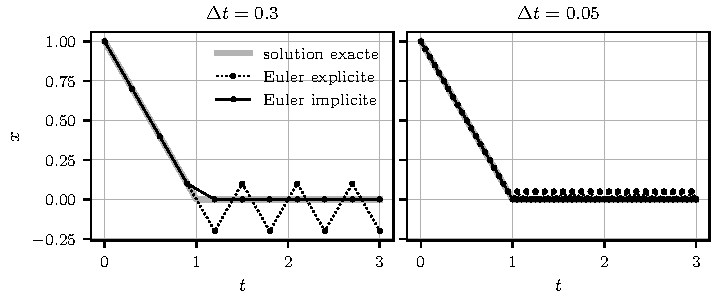
\includegraphics[width=\linewidth]{images/frottement_sec.py.pdf}
\caption{Simulation de \(\dot{x}=-\mathrm{sign}(x)\), \(x(0)=1\), par
les schémas d'Euler explicite et implicite avec \({\Delta t}=0{,}3\)
(à gauche) et \({\Delta t}=0{,}05\) (à droite). Le schéma explicite
oscille indéfiniment autour de 0 avec une amplitude \({\Delta t}\)
(chattering)\,; le schéma implicite s'arrête exactement en 0. 
%Le code
%générant cette figure est
%\texttt{images/frottement\_sec.py}.
}\label{ed2-fig_frottement_sec}
}
\end{figure}

\hypertarget{ed2-euler-symplectique}{%
\section{Euler symplectique}\label{ed2-euler-symplectique}}

\hypertarget{ed2-answer-symp-1}{%
\subsubsection*{Question 1}\label{ed2-answer-symp-1}}

\addcontentsline{toc}{subsubsection}{Question 1}

Dans le cas d'Euler explicite, \(x^{j+1}=Ax^j\) avec \[
A = \left(
\begin{matrix}
1 & {\Delta t}\\
-{\Delta t}\, \omega^2 & 1
\end{matrix}
\right)
\] dont les valeur propres sont \(1 \pm i\omega {\Delta t}\) de norme
\(\sqrt{1+{\Delta t}^2 \, \omega^2}>1\). Donc les solutions divergent.

Dans le cas d'Euler implicite, \(x^{j+1}=Ax^j\) avec \[
A = \frac{1}{1+{\Delta t}^2 \, \omega^2} \left(
\begin{matrix}
1 & {\Delta t}\\
-{\Delta t}\, \omega^2 & 1
\end{matrix}
\right)
\] dont les valeurs propres sont \(1/(1 \pm i\omega {\Delta t})\) de
norme \(1/\sqrt{1+{\Delta t}^2 \, \omega^2}<1\). Donc les solutions
convergent vers 0.

Or on peut vérifier que le long des vraies solutions, l'énergie
\(\omega^2 x_1^2 + x_2^2\) est constante donc les trajectoires sont
bornées et ne peuvent pas converger vers zéro. Aucun des deux schémas
n'approxime les solutions correctement sur le long-terme.

\hypertarget{ed2-answer-symp-2}{%
\subsubsection*{Question 2}\label{ed2-answer-symp-2}}

\addcontentsline{toc}{subsubsection}{Question 2}

Le schéma symplectique donne \[
\left( 
  \begin{matrix}
  \omega^2 & 0 \\
  {\Delta t}\, w^2 & 1
  \end{matrix}
\right)
\left( 
  \begin{matrix}
  x_1^{j+1}\\
  x_2^{j+1}
  \end{matrix}
\right)
=
\left( 
  \begin{matrix}
  \omega^2 & {\Delta t}\, w^2 \\
  0 & 1
  \end{matrix}
\right)
\left( 
  \begin{matrix}
  x_1^{j}\\
  x_2^{j}
  \end{matrix}
\right)
\] En multipliant à gauche alternativement par
\(\left( \begin{matrix}x_1^{j+1} & x_2^{j+1}\end{matrix}\right)\) et
\(\left( \begin{matrix}x_1^{j} & x_2^{j}\end{matrix}\right)\), on
obtient \begin{align*}
\omega^2 (x_1^{j+1})^2 + (x_2^{j+1})^2 +{\Delta t}\, \omega^2 x_1^{j+1}x_2^{j+1}
&= \omega^2 x_1^{j+1} x_1^j + x_2^{j+1}x_2^j +{\Delta t}\, \omega^2 x_1^{j+1}x_2^{j} \\
&= \omega^2 (x_1^{j})^2 + (x_2^{j})^2 +{\Delta t}\, \omega^2 x_1^{j}x_2^{j} 
\end{align*} et donc la quantité
\(\omega^2 x_1^2 + x_2^2 +{\Delta t}\, \omega^2 x_1x_2\) est bien
constante. Pour \(\omega^2-\frac{{\Delta t}^2 \omega^4}{4}>0\), soit
\(\omega {\Delta t}<2\), cette matrice est définie positive, donc les
solutions restent sur une ellipse. Cette ellipse se rapproche de la
vraie solution lorsque \({\Delta t}\) tend vers 0. Ce schéma est donc
approprié pour simuler les trajectoires sur un temps long. Les trois
schémas sont comparés sur la
\protect\hyperlink{ed2-fig_oscillateur_symplectique}{Figure~\ref*{ed2-fig_oscillateur_symplectique}
(p. \pageref*{ed2-fig_oscillateur_symplectique})}\,: en quelques
périodes, Euler explicite spirale vers l'extérieur et Euler implicite
vers l'origine, tandis qu'Euler symplectique reste sur une ellipse proche
du cercle exact. Son énergie \(\omega^2 x_1^2 + x_2^2\) n'est pas
exactement constante, mais oscille sans dériver\,; c'est la quantité
modifiée \(\omega^2 x_1^2 + x_2^2 +{\Delta t}\, \omega^2 x_1x_2\) qui
est conservée.

\begin{figure}
\hypertarget{ed2-fig_oscillateur_symplectique}{%
\centering
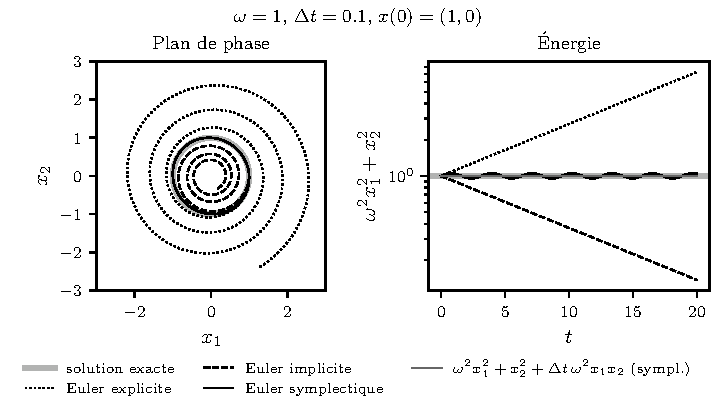
\includegraphics[width=\linewidth]{images/oscillateur_symplectique.py.pdf}
\caption{Simulation de l'oscillateur \(\dot x_1 = x_2\),
\(\dot x_2 = -\omega^2 x_1\) par les schémas d'Euler explicite, implicite
et symplectique (\(\omega=1\), \({\Delta t}=0{,}1\), trois périodes). 
%A gauche, le plan de phase\,; à droite, l'énergie \(\omega^2 x_1^2 + x_2^2\) le long des solutions numériques, en échelle logarithmique. Le code générant cette figure est \texttt{images/oscillateur\_symplectique.py}.
}\label{ed2-fig_oscillateur_symplectique}
}
\end{figure}

\hypertarget{ed2-answer-symp-3}{%
\subsubsection*{Question 3}\label{ed2-answer-symp-3}}

\addcontentsline{toc}{subsubsection}{Question 3}

L'algorithme symplectique est décrit par \(x^{j+1}=Ax^j\) avec \[
A = \left(
\begin{matrix}
1 & {\Delta t}\\
-{\Delta t}\, \omega^2 & 1-{\Delta t}^2 \, \omega^2
\end{matrix}
\right)
\] dont le polynôme caractéristique s'écrit \[
s^2 - (2-{\Delta t}^2 \, \omega^2) s + 1
\] On a les cas suivants~:

\begin{itemize}
\item
  si \((2-{\Delta t}^2 \, \omega^2)^2 -4 <0\), i.e., si
  \(\omega {\Delta t}<2\), les valeurs propres sont imaginaires
  conjuguées et de module 1.
\item
  si \(\omega {\Delta t}> 2\), les valeurs propres sont réelles de
  produit 1, donc l'une est supérieure à 1 est le schéma diverge.
\item
  dans le cas extrême où \(\omega {\Delta t}= 2\), il y a une valeur
  propre double en -1.
\end{itemize}

\hypertarget{ed2-answer-symp-4}{%
\subsubsection*{Question 4}\label{ed2-answer-symp-4}}

\addcontentsline{toc}{subsubsection}{Question 4}

Pour un système hamiltonien, on peut donc proposer \begin{align*}
q^{j+1} &= q^{j} + {\Delta t}\, \nabla_p H(q^{j},p^{j}) \\
p^{j+1} &= p^{j} - {\Delta t}\, \nabla_q H(q^{j+1},p^{j+1})
\end{align*} ou bien \begin{align*}
q^{j+1} &= q^{j} + {\Delta t}\, \nabla_p H(q^{j+1},p^{j+1}) \\
p^{j+1} &= p^{j} - {\Delta t}\, \nabla_q H(q^{j},p^j)
\end{align*} pour \({\Delta t}\) suffisamment petit. C'est cet algorithme qui est utilis\'e dans la \protect\hyperlink{ed2-fig_systeme_solaire}{Figure~\ref*{ed2-fig_systeme_solaire} (p.
\pageref*{ed2-fig_systeme_solaire})}


\fi

\end{document}
